\documentclass[../../thesis.tex]{subfiles}

\begin{document}

In this thesis, we focus on two main objectives, which relates back to the research questions. Firstly, in Stage 1, we aim to determine whether NC-VQVAE can learn more expressive representations compared to VQVAE. Specifically, we investigate whether NC-VQVAE can achieve reconstruction performance on par with VQVAE while simultaneously enhancing downstream classification. In Stage 2, our interest lies in examining the impact of NC-VQVAE on time series generation.\newline

Our evaluation process begins with assessing the tokenization models, focusing on their reconstruction capability and performance in downstream classification tasks. Subsequently, we then evaluate the performance of the generative models using metrics such as IS (Inception Score), FID (Fréchet Inception Distance), and CAS (Classification Accuracy Score). Additionally, visual inspections are conducted to provide further insights into the models' performance.

\section{Stage 1}
% In this section we present the results of the tokenization model, in particular the reconstruction loss and the downstream classification accuracy. We address research question 1 and 2, if the proposed NC-VQVAE is able to reconstruct on par with the naive VQVAE and if the learned latent representations are more expressive, in the sense that they simultaneously improve the downstream classification accuracy. We see that some configuration of NC-VQVAE is the top performer on the majority of datasets for both metrics, and provides significant increase in probe accuracy. 


In this section, we present the findings concerning the tokenization model. We find that some configuration of NC-VQVAE outperform naive VQVAE across the majority of datasets, both in terms of reconstruction quality and downstream classification, providing significant improvements in probe accuracy.

\subsection{Reconstruction}

We present the top 1 and mean reconstruction losses across the four runs in Table \ref{tab:best_recons} and Table \ref{tab:mean_recons}, respectively.

\begin{table}[H]
    \centering
    \title{Mean validation reconstruction error}
    \begin{adjustbox}{width=\textwidth}
    \begin{tabular}{lc|c|c|c|c|c|c} % 8 cols, 1 for dataset, 7 for val_recons across models (7 models)
        \toprule
        \multirow{3}{*}{\textbf{Dataset}} & \multicolumn{1}{c}{\textbf{Baseline}} & \multicolumn{6}{c}{\textbf{SSL Method}} \\
                                         \cmidrule(lr){3-8}
                                          & \multicolumn{1}{c}{Regular}           & \multicolumn{3}{c}{Barlow Twins}    &  \multicolumn{3}{c}{VIbCReg} \\
                                                                                   \cmidrule(lr){3-5}                    \cmidrule(lr){6-8}
                                          &   None                                & Warp  & Slice & Gauss               & Warp & Slice & Gauss \\
                            
        \midrule
        FordA                   & 0.217 & 0.127 & 0.134 & \textbf{0.108} & 0.173 & 0.169 & 0.203 \\
        ElectricDevices         & \textbf{0.041} & 0.067 & 0.044 & 0.049 & 0.105 & 0.042 & 0.049 \\
        StarLightCurves         & \textbf{0.032} & 0.042 & 0.069 & 0.071 & 0.052 & 0.050 & 0.068 \\
        Wafer                   & 0.044 & 0.037 & 0.048 & 0.049 & \textbf{0.035} & 0.042 & 0.039 \\
        ECG5000                 & \textbf{0.048} & 0.083 & 0.170 & 0.104 & 0.093 & 0.205 & 0.064 \\
        TwoPatterns             & 0.197 & 0.201 & \textbf{0.184} & 0.230 & 0.214 & 0.186 & 0.207 \\
        UWaveGestureLibraryAll  & 0.190 & \textbf{0.172} & 0.190 & 0.245 & 0.189 & 0.178 & 0.237 \\
        FordB                   & 0.150 & 0.115 & 0.122 & 0.123 & \textbf{0.114} & 0.121 & 0.142 \\
        ShapesAll               & \textbf{0.045} & 0.056 & 0.066 & 0.102 & 0.064 & 0.069 & 0.073 \\
        SonyAIBORobotSurface1   & 0.402 & 0.509 & 0.494 & 0.491 & \textbf{0.360} & 0.363 & 0.418 \\
        SonyAIBORobotSurface2   & 0.623 & 0.622 & 0.618 & 0.640 & 0.487 & \textbf{0.454} & 0.589 \\
        Symbols                 & 0.110 & 0.143 & 0.134 & 0.173 & 0.078 & \textbf{0.067} & 0.105 \\
        Mallat                  & 0.066 & 0.081 & 0.091 & 0.096 & 0.066 & 0.067 & \textbf{0.060} \\
        \bottomrule
    \end{tabular}
    \end{adjustbox}
    \caption{Mean validation reconstruction error across all 13 datasets. Results are averaged over four runs.}
    \label{tab:mean_recons}
\end{table}

\begin{table}[H]
    \centering
    \title{Top 1 validation reconstruction error}
    \begin{adjustbox}{width=\textwidth}
    \begin{tabular}{lc|c|c|c|c|c|c} % 8 cols, 1 for dataset, 7 for val_recons across models (7 models)
        \toprule
        \multirow{3}{*}{\textbf{Dataset}} & \multicolumn{1}{c}{\textbf{Baseline}} & \multicolumn{6}{c}{\textbf{SSL Method}} \\
                                         \cmidrule(lr){3-8}
                                          & \multicolumn{1}{c}{Regular}           & \multicolumn{3}{c}{Barlow Twins}    &  \multicolumn{3}{c}{VIbCReg} \\
                                                                                   \cmidrule(lr){3-5}                    \cmidrule(lr){6-8}
                                          &   None                                & Warp  & Slice & Gauss               & Warp & Slice & Gauss \\
                            
        \midrule
        FordA                   & 0.158 & 0.108 & 0.111 & \textbf{0.087} & 0.130 & 0.134 & 0.113 \\
        ElectricDevices         & 0.036 & 0.060 & 0.034 & 0.043 & 0.092 & \textbf{0.031} & 0.045 \\
        StarLightCurves         & \textbf{0.026} & 0.037 & 0.057 & 0.055 & 0.043 & 0.048 & 0.065 \\
        Wafer                   & 0.038 & 0.031 & 0.045 & 0.043 & \textbf{0.027} & 0.031 & 0.038 \\
        ECG5000                 & \textbf{0.044} & 0.069 & 0.156 & 0.084 & 0.080 & 0.181 & 0.056 \\
        TwoPatterns             & 0.181 & 0.184 & \textbf{0.169} & 0.208 & 0.200 & 0.172 & 0.185 \\
        UWaveGestureLibraryAll  & 0.159 & \textbf{0.145} & 0.167 & 0.201 & 0.155 & 0.169 & 0.233 \\
        FordB                   & 0.117 & 0.094 & 0.090 & 0.103 & \textbf{0.082} & 0.094 & 0.102 \\
        ShapesAll               & \textbf{0.035} & 0.043 & 0.046 & 0.092 & 0.061 & 0.063 & 0.067 \\
        SonyAIBORobotSurface1   & 0.381 & 0.473 & 0.472 & 0.465 & 0.329 & \textbf{0.328} & 0.408 \\
        SonyAIBORobotSurface2   & 0.513 & 0.577 & 0.536 & 0.588 & 0.444 & \textbf{0.414} & 0.470 \\
        Symbols                 & 0.088 & 0.111 & 0.122 & 0.150 & 0.062 & \textbf{0.059} & 0.090 \\
        Mallat                  & 0.061 & 0.075 & 0.076 & 0.088 & 0.059 & 0.059 & \textbf{0.057} \\

  
        \bottomrule
    \end{tabular}
    \end{adjustbox}
    \caption{Top 1 validation reconstruction error across all 13 datasets. Lowest value of the four runs for each model is selected.}
    \label{tab:best_recons}
\end{table}

It's evident that NC-VQVAE achieves comparable reconstruction performance to the baseline model, and certain configurations even outperform the naive VQVAE in terms of mean reconstruction loss for 9 out of 13 datasets.\newline

In Figure \ref{fig:Mean_val_recons}, we observe minimal differences in reconstruction loss across most datasets, regardless of SSL methods and augmentations. However, VIbCReg generally demonstrates slightly better performance compared to Barlow Twins, except for FordA. Additionally, the use of Gaussian augmentation introduces less regularization compared to the other augmentation methods, except for Slice and Shuffle on ECG5000. These findings suggest that incorporating a non-contrastive loss does not compromise the reconstruction capabilities compared to naive VQVAE. \newline

\begin{figure}[h]
    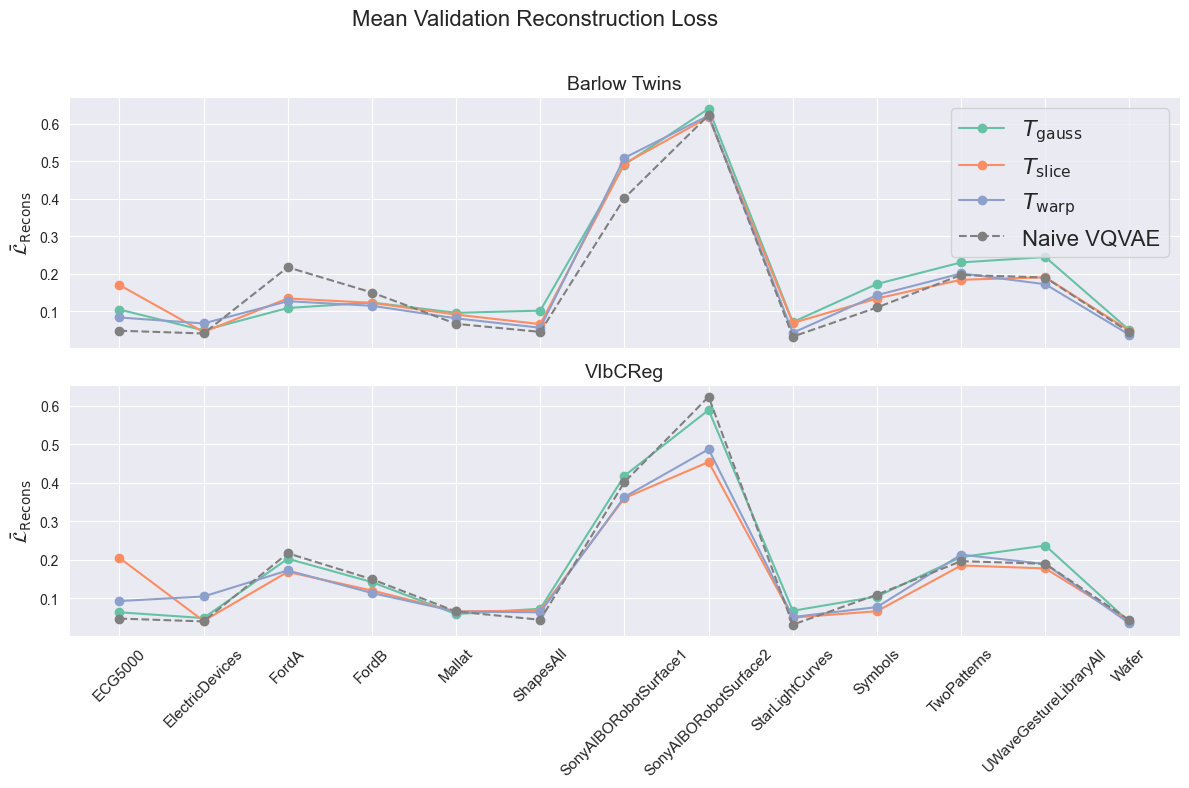
\includegraphics[scale=0.4]{Mean_val_recons.png}
    \centering  
    \caption{Mean validation reconstruction loss for the two models, compared to naive VQVAE}
    \label{fig:Mean_val_recons}
\end{figure}

To explore the impact of the reconstruction loss of the augmented branch on validation reconstruction, a small ablation stydy was conducted, which is presented in Section \ref{Section:Ablation}. The results indicate that the validation reconstruction loss is robust to the specific value of the augmentation reconstruction weight, indicating a minor role played.\newline

Through investigation into the development of validation reconstruction loss during training, we observed that the right configuration for NC-VQVAE can serve as a regularizer. This is illustrated in Figure \ref{fig:FordA_val_recons} which depicts the development on FordA. 

\begin{figure}[h]
    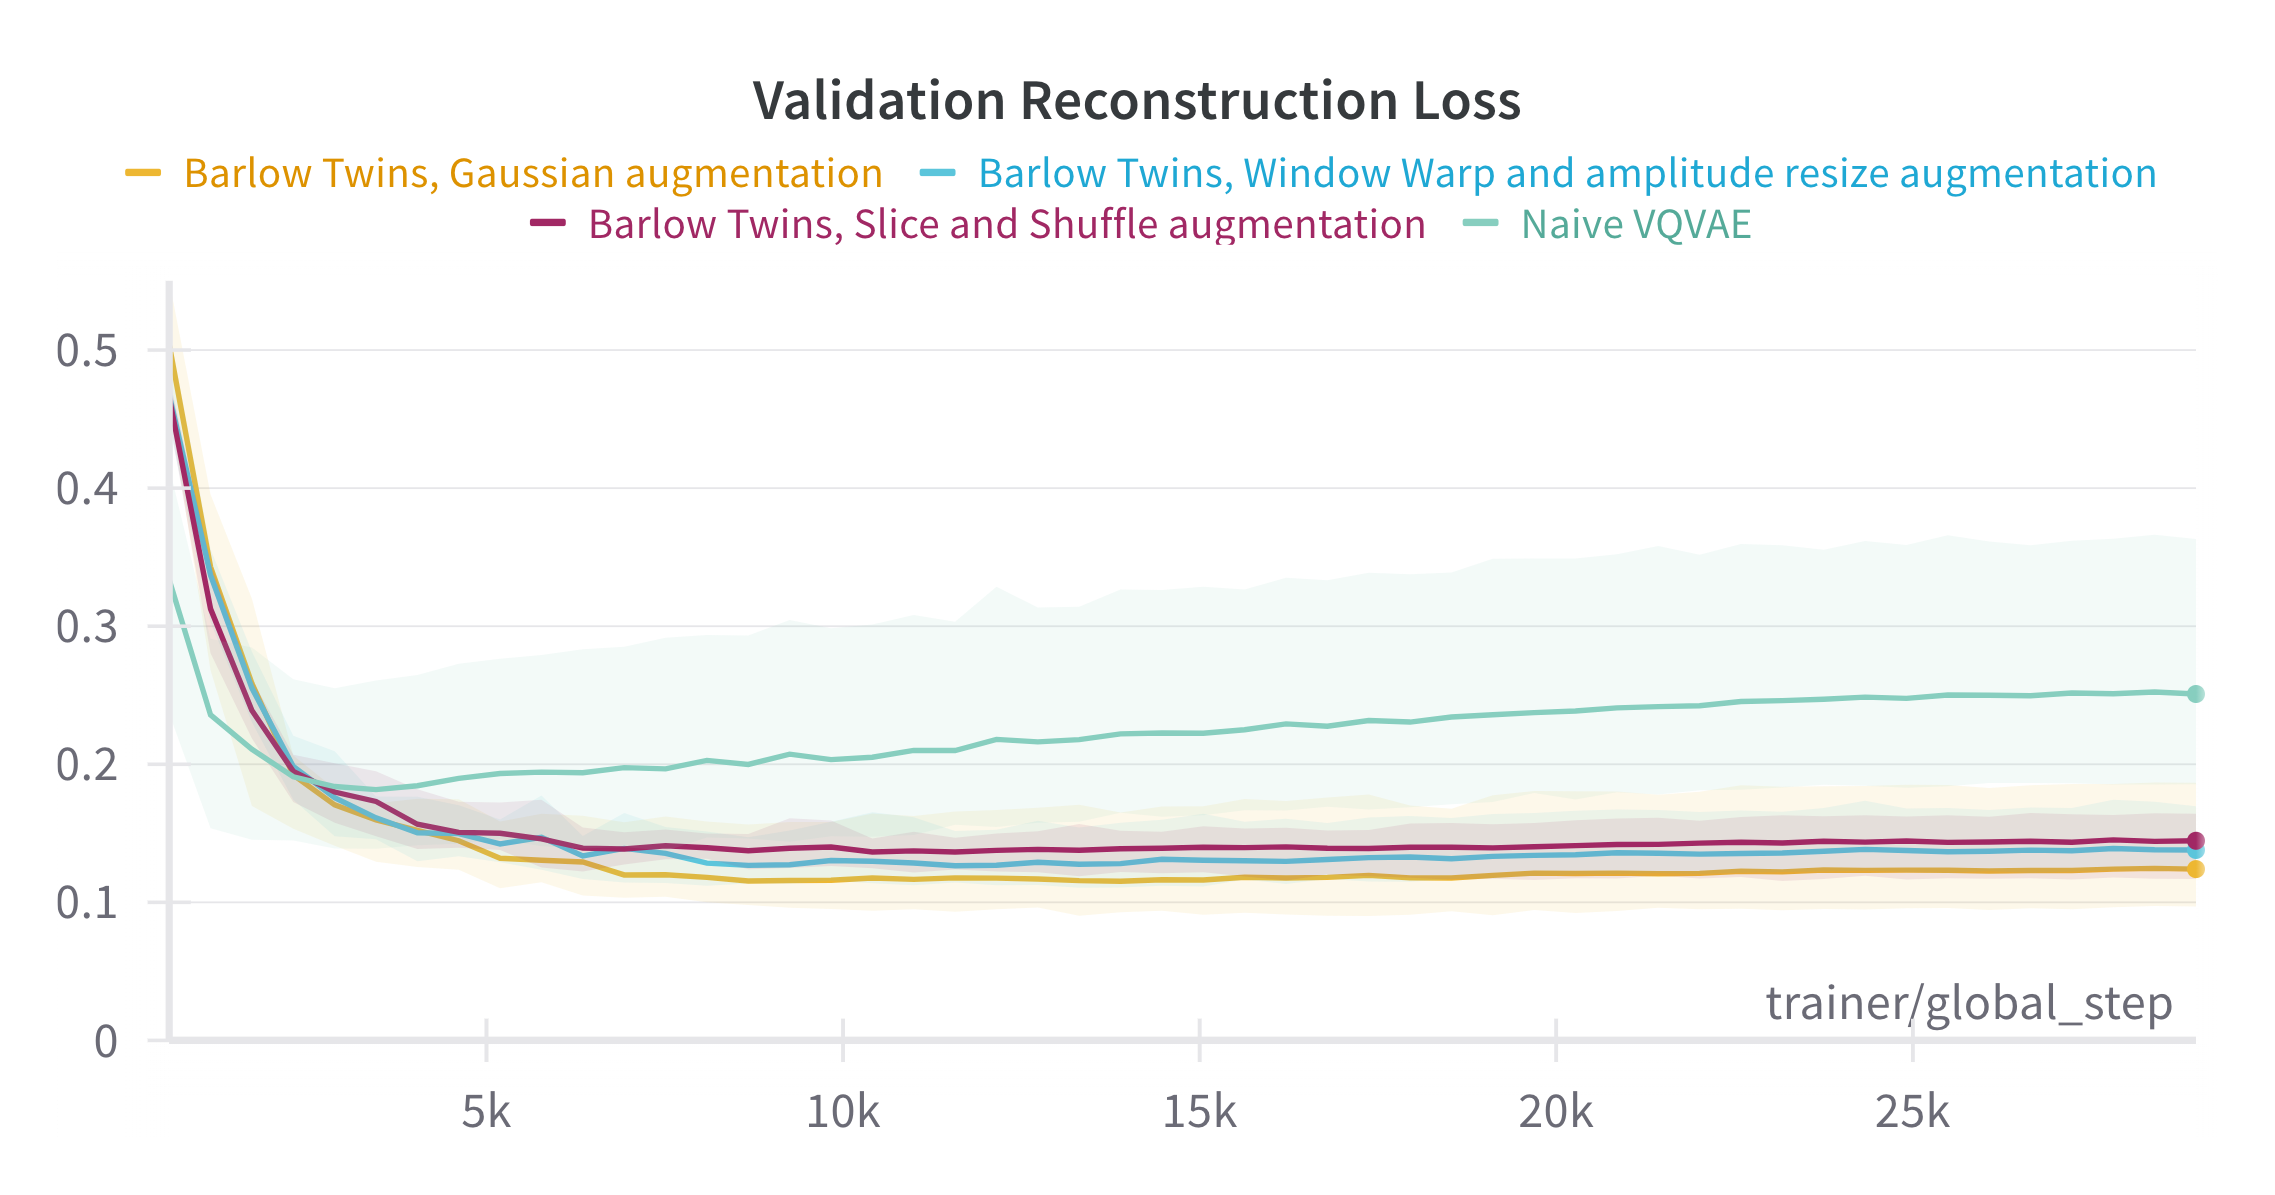
\includegraphics[scale=0.10]{FordA_val_recons.png}
    \centering  
    \caption{Development of the validation reconstruction loss for Barlow Twins and naive VQVAE on FordA during training. Averaged across all four runs. }
    \label{fig:FordA_val_recons}
\end{figure}


\subsection{Classification}

We present the mean and top 1 downstream classification accuracy in Table \ref{tab:mean_probe} and Table \ref{tab:best_probe}, respectively. 


\begin{table}[h]
    \centering
    \title{Mean linear probe accuracy}
    \begin{adjustbox}{width=\textwidth}
    \begin{tabular}{lcc|cc|cc|cc|cc|cc|cc} % 15 cols, 1 for dataset, 14 for svm/knn across models (7 models)
        \toprule
        \multirow{4}{*}{\textbf{Dataset}} & \multicolumn{2}{c}{\textbf{Baseline}} & \multicolumn{12}{c}{\textbf{SSL Method}} \\
                                            \cmidrule(lr){2-3} \cmidrule(lr){4-15}
                                          & \multicolumn{2}{c}{Regular}           & \multicolumn{6}{c}{Barlow Twins}                                                 &  \multicolumn{6}{c}{VIbCReg} \\
                                          \cmidrule(lr){2-3} \cmidrule(lr){4-9} \cmidrule(lr){10-15}
                                          &   \multicolumn{2}{c}{None}            & \multicolumn{2}{c}{Warp}  & \multicolumn{2}{c}{Slice} & \multicolumn{2}{c}{Gauss} & \multicolumn{2}{c}{Warp} & \multicolumn{2}{c}{Slice} & \multicolumn{2}{c}{Gauss} \\
                                          \cmidrule(lr){2-3} \cmidrule(lr){4-5} \cmidrule(lr){6-7} \cmidrule(lr){8-9} \cmidrule(lr){10-11} \cmidrule(lr){12-13}\cmidrule(lr){14-15}
                                          & KNN & SVM                               & KNN & SVM                  & KNN & SVM                & KNN & SVM                 & KNN & SVM                 & KNN & SVM                 & KNN & SVM   \\
        \midrule
        FordA                   & 0.70 & 0.74 & 0.83 & 0.84 & \textbf{0.91} & \textbf{0.89} & 0.80 & 0.83 & 0.80 & 0.74 & 0.87 & 0.86 & 0.76 & 0.78 \\
        ElectricDevices         & 0.35 & 0.41 & 0.35 & \textbf{0.44} & 0.38 & 0.41 & \textbf{0.40} & 0.42 & 0.33 & 0.38 & 0.36 & 0.39 & 0.39 & 0.43 \\
        StarLightCurves         & 0.87 & 0.89 & 0.93 & 0.93 & \textbf{0.94} & \textbf{0.94} & 0.88 & 0.88 & 0.92 & \textbf{0.94} & 0.91 & 0.93 & 0.89 & 0.89 \\
        Wafer                   & 0.93 & 0.89 & 0.96 & \textbf{0.94} & 0.96 & \textbf{0.94} & 0.96 & 0.93 & \textbf{0.97} & 0.94 & 0.96 & 0.92 & \textbf{0.97} & 0.92 \\
        ECG5000                 & 0.80 & 0.83 & 0.85 & 0.81 & \textbf{0.88} & 0.84 & 0.86 & \textbf{0.84} & 0.86 & 0.82 & \textbf{0.88} & \textbf{0.84} & 0.84 & 0.82 \\
        TwoPatterns             & 0.34 & 0.53 & \textbf{0.69} &\textbf{ 0.91} & 0.66 & 0.82 & 0.47 & 0.71 & 0.64 & 0.90 & 0.68 & 0.80 & 0.55 & 0.72 \\
        UWaveGestureLibraryAll  & 0.31 & 0.40 & \textbf{0.62} & 0.70 & 0.56 & 0.63 & 0.40 & 0.54 & \textbf{0.62} & \textbf{0.73} & 0.55 & 0.66 & 0.44 & 0.55 \\
        FordB                   & 0.58 & 0.60 & 0.64 & 0.67 & 0.74 & 0.76 & 0.64 & 0.68 & 0.63 & 0.64 & 0.70 & 0.70 & 0.61 & 0.64\\
        ShapesAll               & 0.29 & 0.30 & 0.49 & 0.55 & 0.53 & \textbf{0.60} & 0.40 & 0.48 & 0.48 & 0.56 &\textbf{ 0.54} & \textbf{0.60} & 0.40 & 0.46 \\
        SonyAIBORobotSurface1   & 0.56 & 0.68 & 0.54 & 0.70 & \textbf{0.61} & \textbf{0.74} & 0.53 & 0.70 & 0.48 & \textbf{0.74} & 0.58 & 0.71 & 0.54 & 0.69 \\
        SonyAIBORobotSurface2   & \textbf{0.81} & \textbf{0.86} & 0.77 & 0.79 & 0.80 & 0.80 & 0.80 & 0.81 & 0.77 & 0.85 & 0.80 & 0.85 & 0.80 & 0.85  \\
        Symbols                 & 0.50 & 0.60 & \textbf{0.59} & 0.60 & 0.50 & \textbf{0.66} & \textbf{0.59} & \textbf{0.66} & 0.45 & 0.61 & 0.42 & 0.62 & 0.43 & 0.63 \\
        Mallat                  & 0.63 & 0.77 & 0.72 & 0.81 & 0.76 & 0.83 & 0.68 & 0.78 & \textbf{0.79} & \textbf{0.87} & 0.77 & 0.85 & 0.69 & \textbf{0.86} \\
        \bottomrule
    \end{tabular}
    \end{adjustbox}
    
    \caption{Summary of mean linear probe accuracy by SSL Method and Augmentation. Average across 4 seeds. Best result for KNN and SVM are highlighted in bold.}
    \label{tab:mean_probe}
\end{table}

\begin{table}[H]
    \centering
    \title{Top 1 linear probe accuracy}
    \begin{adjustbox}{width=\textwidth}
    \begin{tabular}{lcc|cc|cc|cc|cc|cc|cc} % 15 cols, 1 for dataset, 14 for svm/knn across models (7 models)
        \toprule
        \multirow{4}{*}{\textbf{Dataset}} & \multicolumn{2}{c}{\textbf{Baseline}} & \multicolumn{12}{c}{\textbf{SSL Method}} \\
                                            \cmidrule(lr){2-3} \cmidrule(lr){4-15}
                                          & \multicolumn{2}{c}{Regular}           & \multicolumn{6}{c}{Barlow Twins}                                                 &  \multicolumn{6}{c}{VIbCReg} \\
                                          \cmidrule(lr){2-3} \cmidrule(lr){4-9} \cmidrule(lr){10-15}
                                          &   \multicolumn{2}{c}{None}            & \multicolumn{2}{c}{Warp}  & \multicolumn{2}{c}{Slice} & \multicolumn{2}{c}{Gauss} & \multicolumn{2}{c}{Warp} & \multicolumn{2}{c}{Slice} & \multicolumn{2}{c}{Gauss} \\
                                          \cmidrule(lr){2-3} \cmidrule(lr){4-5} \cmidrule(lr){6-7} \cmidrule(lr){8-9} \cmidrule(lr){10-11} \cmidrule(lr){12-13}\cmidrule(lr){14-15}
                                          & KNN & SVM                               & KNN & SVM                  & KNN & SVM                & KNN & SVM                 & KNN & SVM                 & KNN & SVM                 & KNN & SVM   \\
        \midrule
        FordA                   & 0.75 & 0.78 & 0.84 & 0.88 & \textbf{0.93} & \textbf{0.92} & 0.85 & 0.87 & 0.81 & 0.77 & 0.88 & 0.90 & 0.86 & 0.85 \\
        ElectricDevices         & 0.35 & 0.43 & 0.36 & 0.45 & 0.39 & 0.43 & \textbf{0.45} & \textbf{0.46} & 0.34 & 0.42 & 0.39 & 0.42 & 0.42 & 0.45 \\
        StarLightCurves         & 0.89 & 0.91 & 0.94 & 0.95 & \textbf{0.96} & \textbf{0.96} & 0.90 & 0.91 & 0.95 & 0.95 & 0.93 & 0.95 & 0.90 & 0.90 \\
        Wafer                   & 0.94 & 0.89 &\textbf{ 0.97} & \textbf{0.95} & \textbf{0.97} & \textbf{0.95} & \textbf{0.97} & 0.93 & \textbf{0.97} & \textbf{0.95} & \textbf{0.97} & \textbf{0.95} & \textbf{0.97} & 0.94 \\
        ECG5000                 & 0.83 & 0.84 & 0.88 & 0.86 & \textbf{0.90} & \textbf{0.88} & \textbf{0.90} & \textbf{0.88} & 0.88 & 0.85 & 0.89 & 0.86 & 0.86 & 0.85 \\
        TwoPatterns             & 0.37 & 0.62 & \textbf{0.75} & \textbf{0.96} & 0.68 & 0.85 & 0.55 & 0.75 & 0.70 & 0.92 & 0.71 & 0.81 & 0.63 & 0.76 \\
        UWaveGestureLibraryAll  & 0.34 & 0.43 & \textbf{0.67} & 0.74 & 0.60 & 0.67 & 0.43 & 0.54 & \textbf{0.67} & \textbf{0.76} & 0.58 & 0.67 & 0.48 & 0.58 \\
        FordB                   & 0.60 & 0.63 & 0.67 & 0.71 & \textbf{0.76} & \textbf{0.80} & 0.69 & 0.74 & 0.67 & 0.65 & 0.74 & 0.77 & 0.63 & 0.68 \\
        ShapesAll               & 0.33 & 0.34 & 0.53 & 0.59 & \textbf{0.59} & \textbf{0.65} & 0.44 & 0.50 & 0.50 & 0.56 & 0.57 & 0.63 & 0.44 & 0.48 \\
        SonyAIBORobotSurface1   & 0.67 & \textbf{0.80} & 0.61 & 0.77 & 0.76 & \textbf{0.80} & 0.60 & 0.74 & 0.51 & 0.79 & 0.63 & 0.75 & 0.63 & 0.75 \\
        SonyAIBORobotSurface2   & \textbf{0.84} & \textbf{0.89} & 0.80 & 0.86 & 0.82 & 0.84 & 0.83 & 0.82 & 0.81 & 0.88 & 0.81 & 0.88 & 0.83 & 0.87 \\
        Symbols                 & 0.56 & 0.66 & 0.65 & 0.69 & 0.55 & 0.73 & \textbf{0.64} & \textbf{0.71} & 0.51 & 0.65 & 0.45 & 0.67 & 0.46 & 0.69 \\
        Mallat                  & 0.54 & 0.88 & 0.57 & 0.87 & 0.74 & 0.89 & 0.66 & 0.80 & 0.74 & \textbf{0.92} & 0.72 & 0.88 & 0.62 & \textbf{0.90} \\


        \bottomrule
    \end{tabular}
    \end{adjustbox}
    
    \caption{Summary of max linear probe accuracy by SSL Method and Augmentation. Maximum value across 4 seeds. Best result for KNN and SVM are highlighted in bold.}
    \label{tab:best_probe}
\end{table}

A clear improvement in probe accuracy is observed with NC-VQVAE compared to the naive VQVAE. Across 12 out of 13 datasets, a configuration of our model performs best, with the only exception showing a negligible one percent difference for both SVM and KNN. The most significant improvements are observed in FordA, FordB, Mallat, ShapesAll, TwoPatterns, and UWaveGestureLibraryAll.\newline

In Figure \ref{fig:Mean_probe}, we observe that while the choice of augmentation has a substantial impact, all options generally lead to significantly improved probe accuracy across most datasets. Notably, both SSL methods yield comparable probe accuracies for a given augmentation, underscoring the importance of selecting appropriate augmentations. \newline
\begin{figure}[h]
    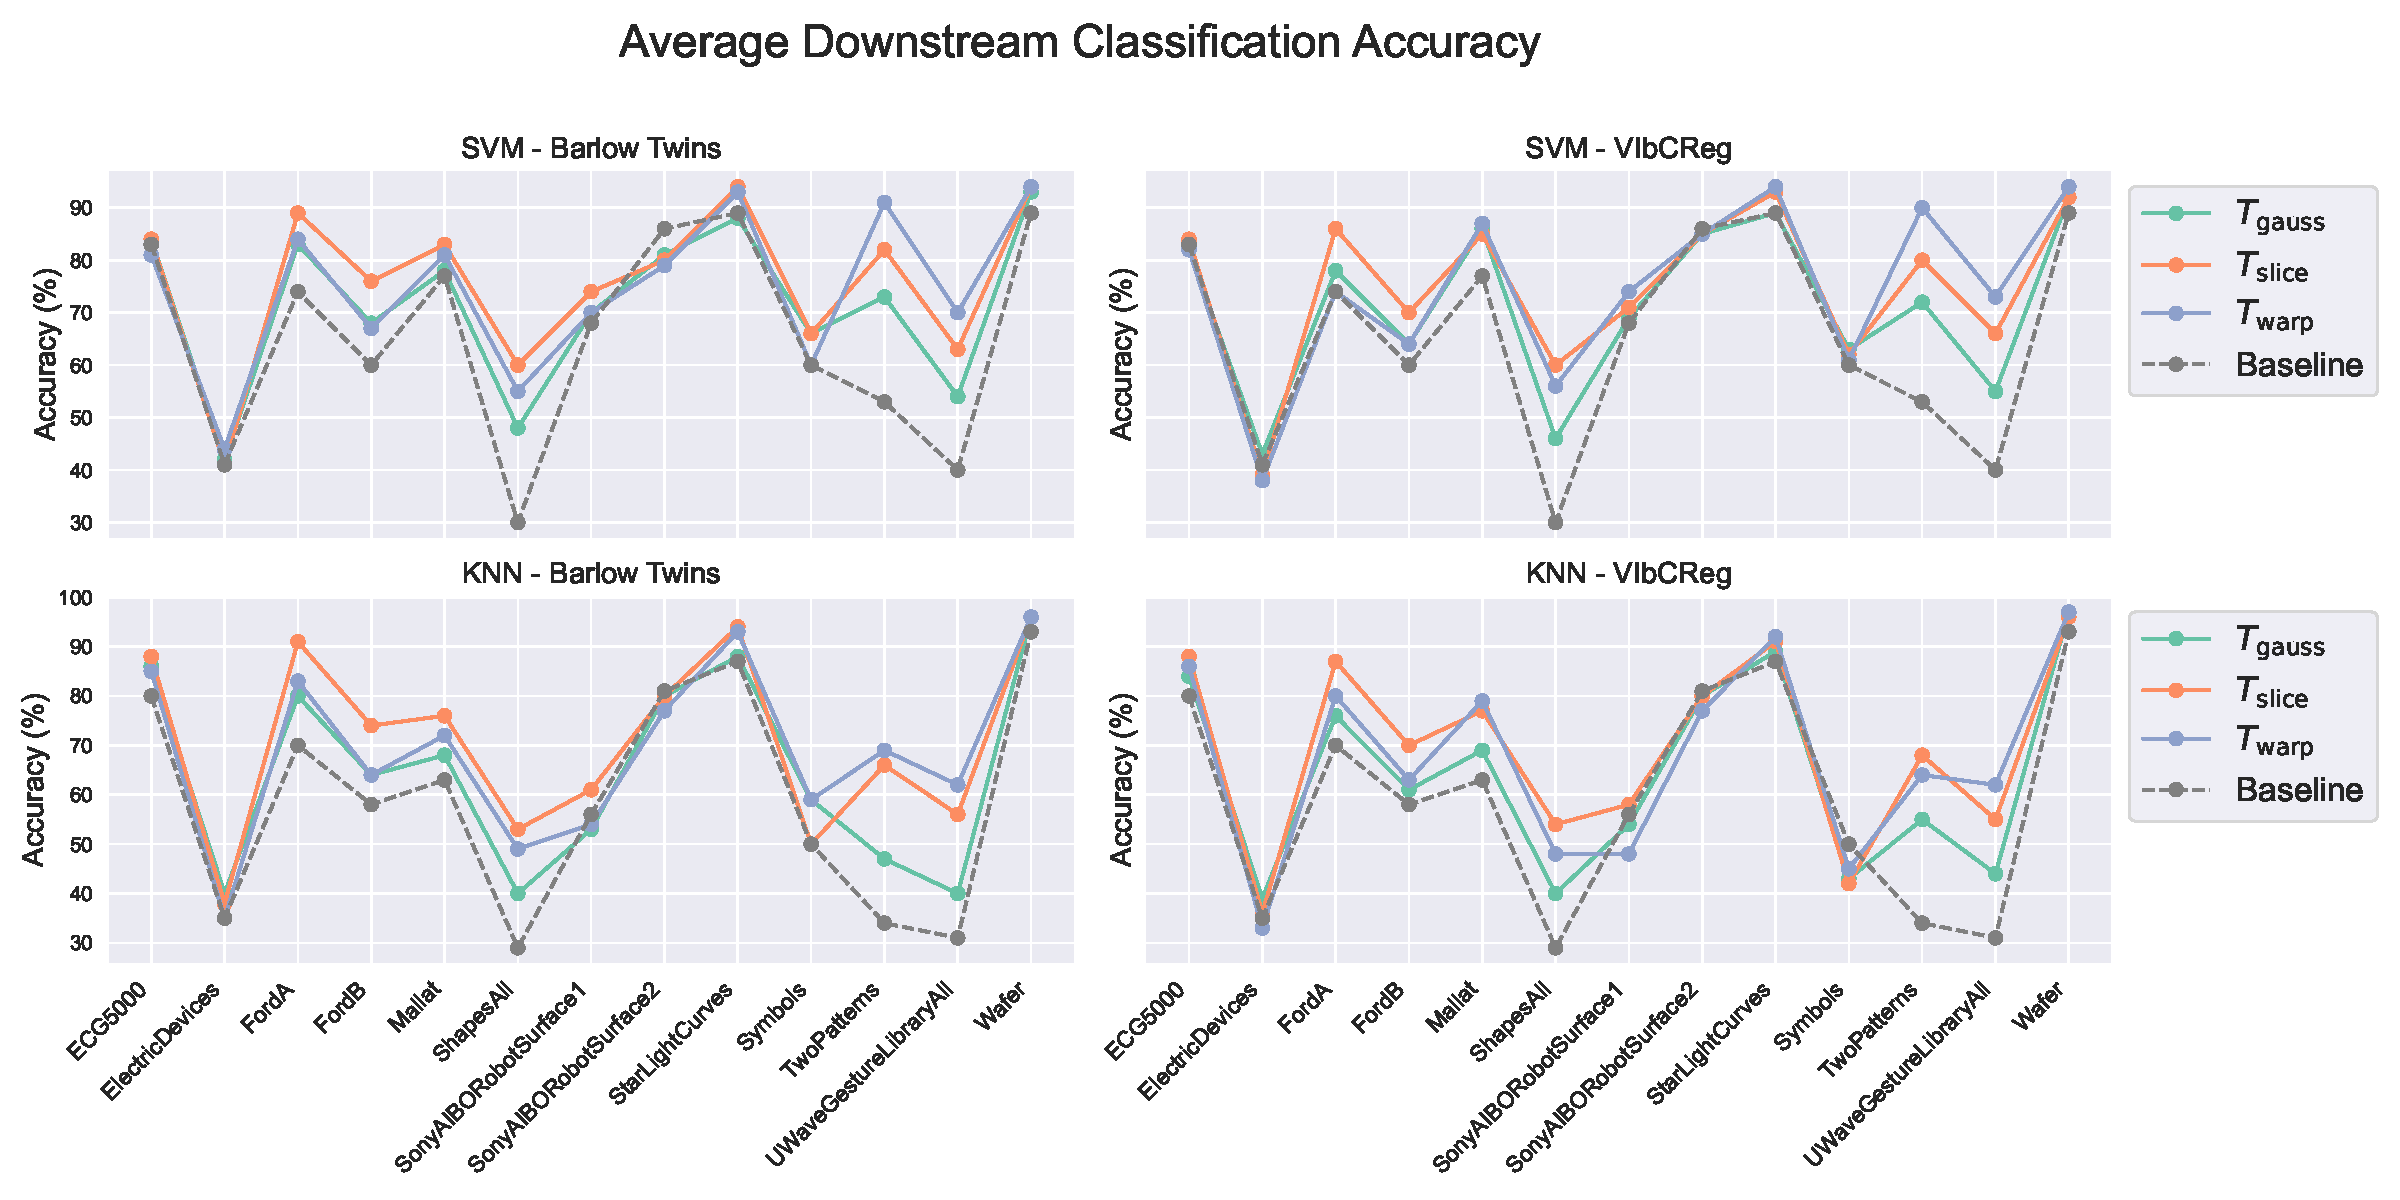
\includegraphics[scale=0.35]{probe_accuracies.pdf}
    \centering  
    \caption{Mean probe accuracies.}
    \label{fig:Mean_probe}
\end{figure}

Further analysis reveals that Slice and Shuffle, as well as Window Warp and Amplitude Resize, result in the most substantial accuracy gains, whereas Gaussian noise consistently yields less pronounced improvements. We hypothesize that since Slice and Warp often generate augmented views that differ considerably from the original, the SSL loss pushes the representations in different directions, potentially leading to better utilization of the latent space. Visualizations in Figure \ref{fig:FordA_TSNE} and \ref{fig:TSNE_TwoPatterns} illustrate the effect of NC-VQVAE on the discrete latent representations of FordA and TwoPatterns. These visualizations demonstrate that representations learned with NC-VQVAE exhibit greater structure than those of the naive VQVAE, with similar samples, typically with the same label, clustered closer together in latent space. This suggests that the SSL loss introduces semantic information into the latent representations.\newline

\begin{figure}[h] 
    \centering
    \begin{minipage}[b]{0.32\textwidth}
        \centering
        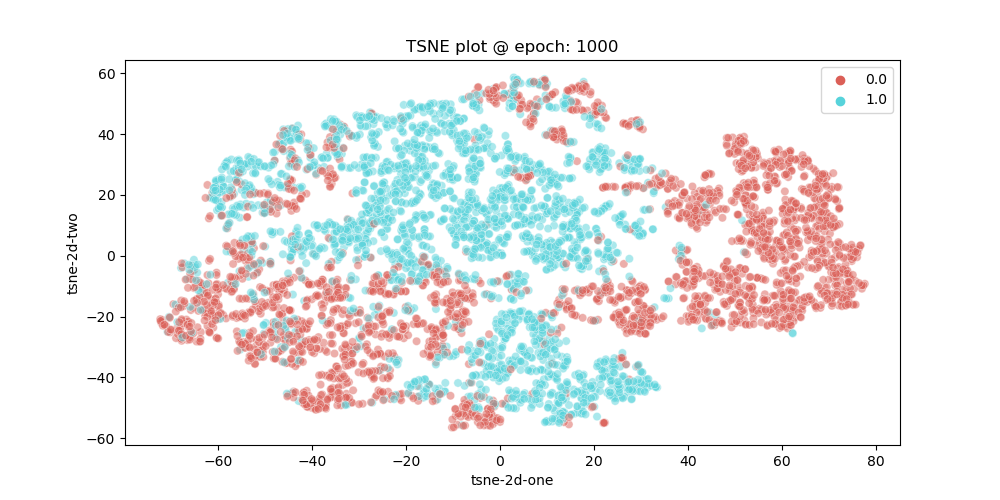
\includegraphics[width=\textwidth]{BT_Slice_FordA_TSNE.png}
    \end{minipage}
    \hfill
    \begin{minipage}[b]{0.32\textwidth}
        \centering
        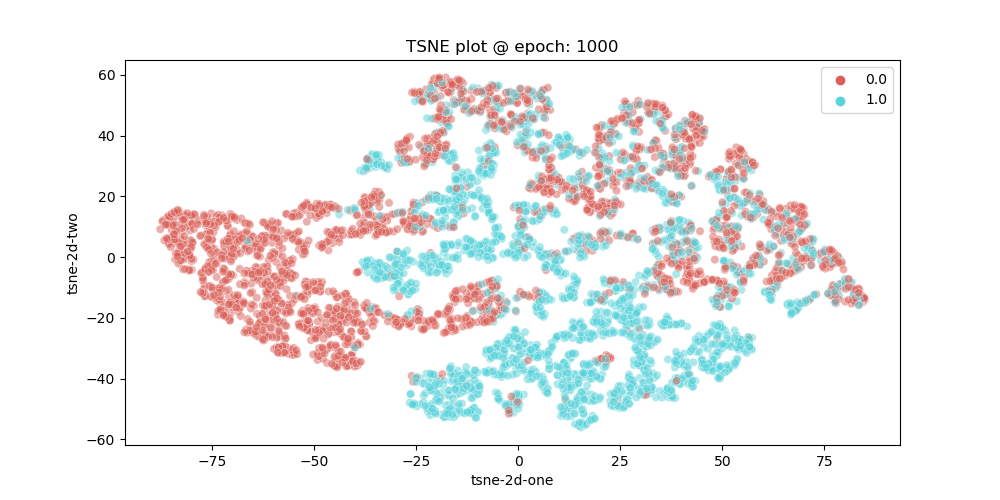
\includegraphics[width=\textwidth]{VIB_Slice_FordA_TSNE.png}
    \end{minipage}
    \hfill
    \begin{minipage}[b]{0.32\textwidth}
        \centering
        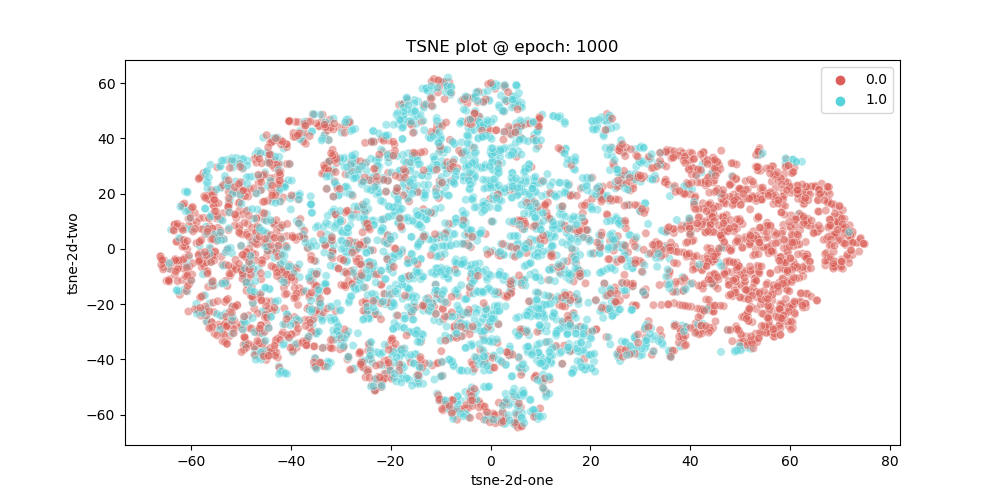
\includegraphics[width=\textwidth]{naive_FordA_TSNE.png}
    \end{minipage}
    \caption{TSNE plots of FordA. Barlow (left) and VIbCReg (center) with Slice and Shuffle, naive VQVAE (right). Best performing model in terms of KNN accuracy is chosen. }
    \label{fig:FordA_TSNE}
\end{figure}


\begin{figure}[h]
    \centering
    \begin{minipage}[b]{0.32\textwidth}
        \centering
        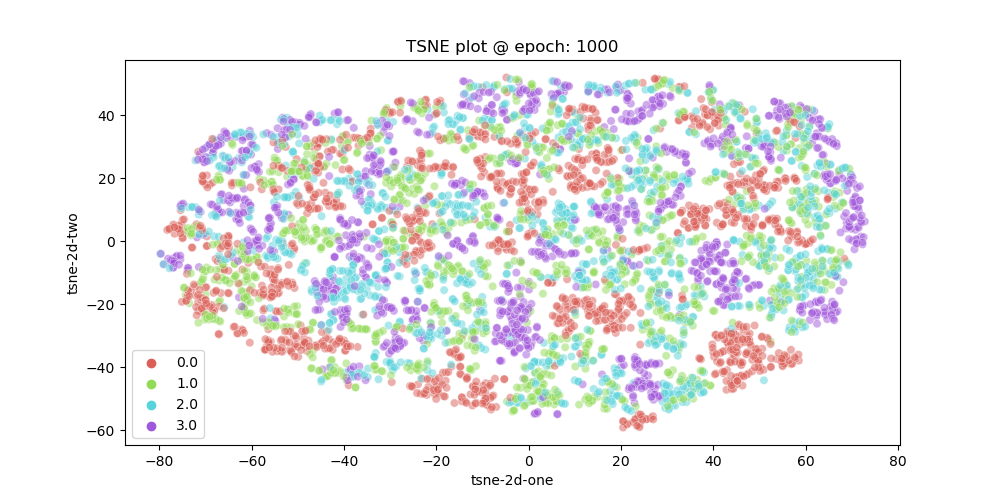
\includegraphics[width=\textwidth]{BT_TwoPatterns_warp_TSNE.png}
    \end{minipage}
    \hfill
    \begin{minipage}[b]{0.32\textwidth}
        \centering
        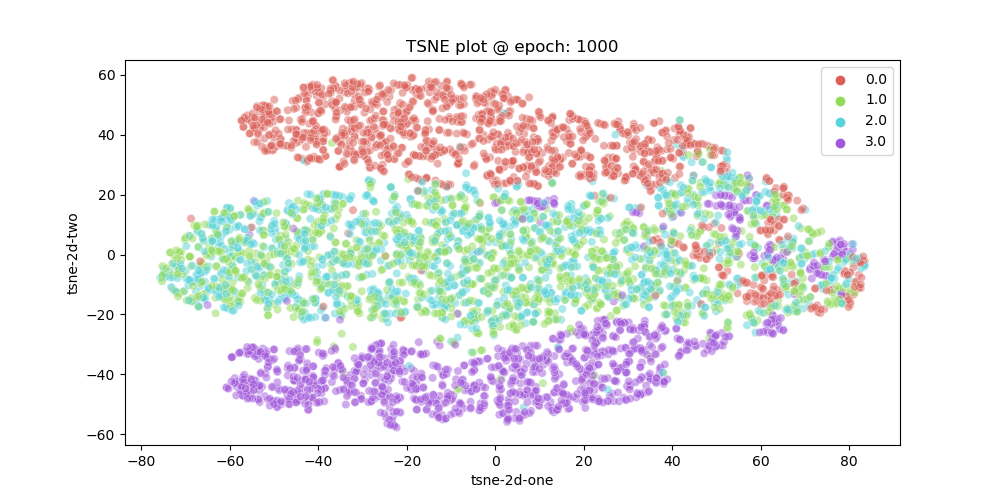
\includegraphics[width=\textwidth]{TSNE_vib_slice_TwoPatterns.png}
    \end{minipage}
    \hfill
    \begin{minipage}[b]{0.32\textwidth}
        \centering
        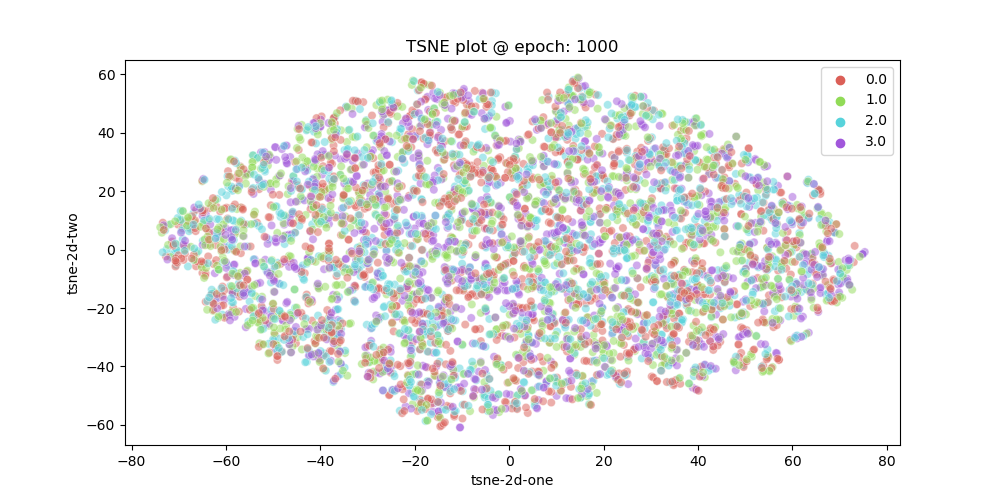
\includegraphics[width=\textwidth]{TSNE_naive_TwoPatterns.png}
    \end{minipage}
    \caption{TSNE plot of discrete latent representations from VIbCReg with Slice and Shuffle (left), Barlow Twins with Window Warp and Amplitude Resize (center) and naive VQVAE (right). Dataset is TwoPatterns. The latent space is significantly more structured with NC-VQVAE.}
    \label{fig:TSNE_TwoPatterns}
\end{figure}

\subsection*{Summary of Stage 1}

In summary, the results from stage 1 indicate that NC-VQVAE can reconstruct on par with the naive VQVAE, and in some cases even improve the reconstruction loss, while substantially improving probe accuracy for most datasets. Addressing research question 1, we conclude that representations learned with NC-VQVAE are more expressive compared to the naive VQVAE, encoding more class-specific information without compromising reconstruction quality. Regarding research question 2, the choice of augmentation plays a pivotal role in the results, with warp and slice typically outperforming gaussian augmentation, particularly in terms of probe accuracy. Additionally, significant variations across datasets support the hypothesis that the optimal choice of augmentations is highly dependent on the dataset.

\subsection{Losses}

We investigate some trends in the development of different loss terms during training. Notably, VIbCReg results in more easily minimizable losses, compared to Barlow Twins, and the Gaussian augmentation results in significantly easier minimization of the SSL loss as well as reducing the VQ loss. In figure \ref{fig:SSL_loss_UWave}, we observe the typical pattern of the SSL loss during training.

\begin{figure}[h]
    \centering
    \begin{minipage}[b]{0.49\textwidth}
        \centering
        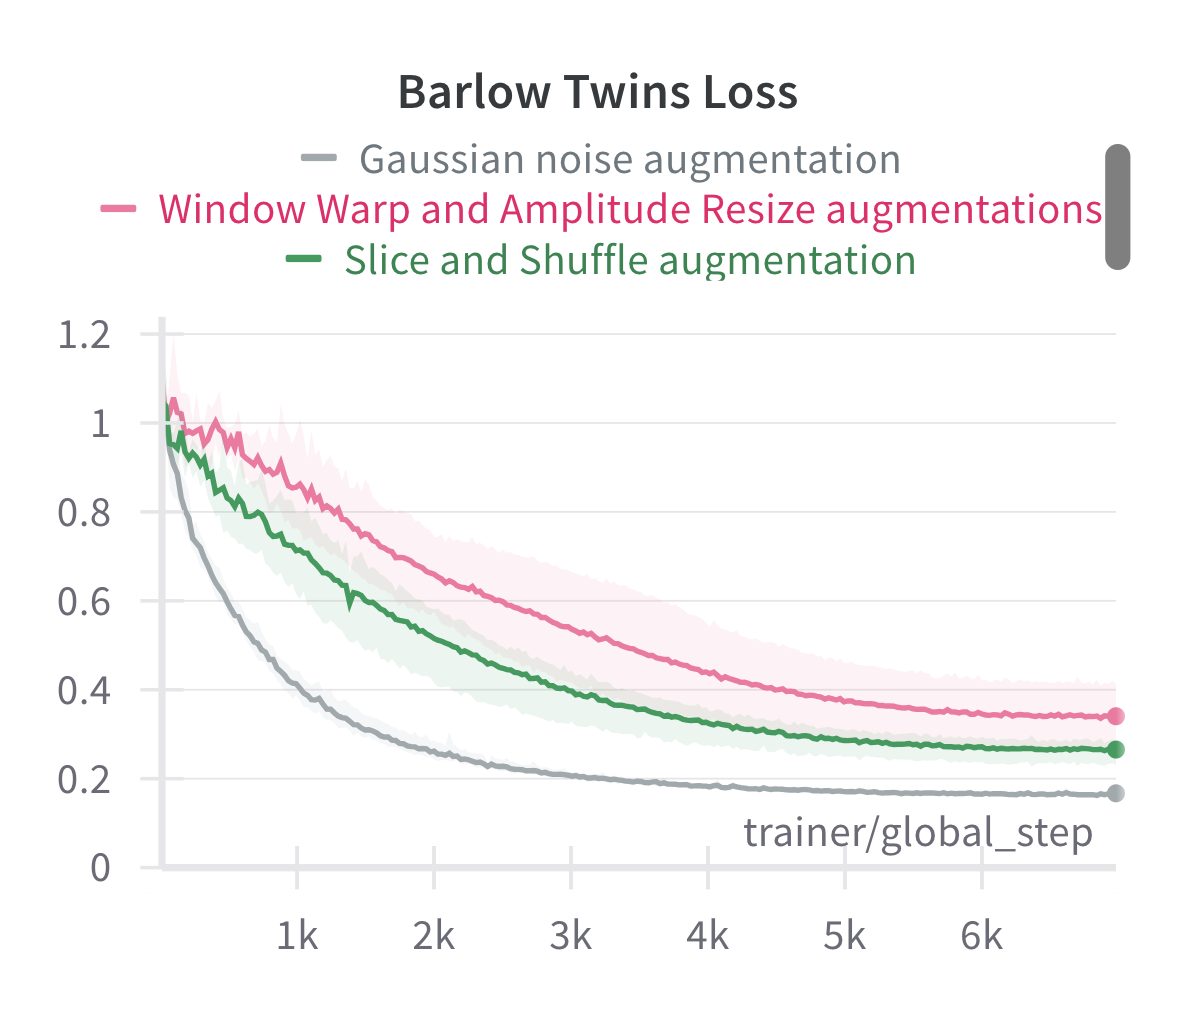
\includegraphics[width=\textwidth]{BT_loss_Uwave.png}
    \end{minipage}
    \hfill
    \begin{minipage}[b]{0.49\textwidth}
        \centering
        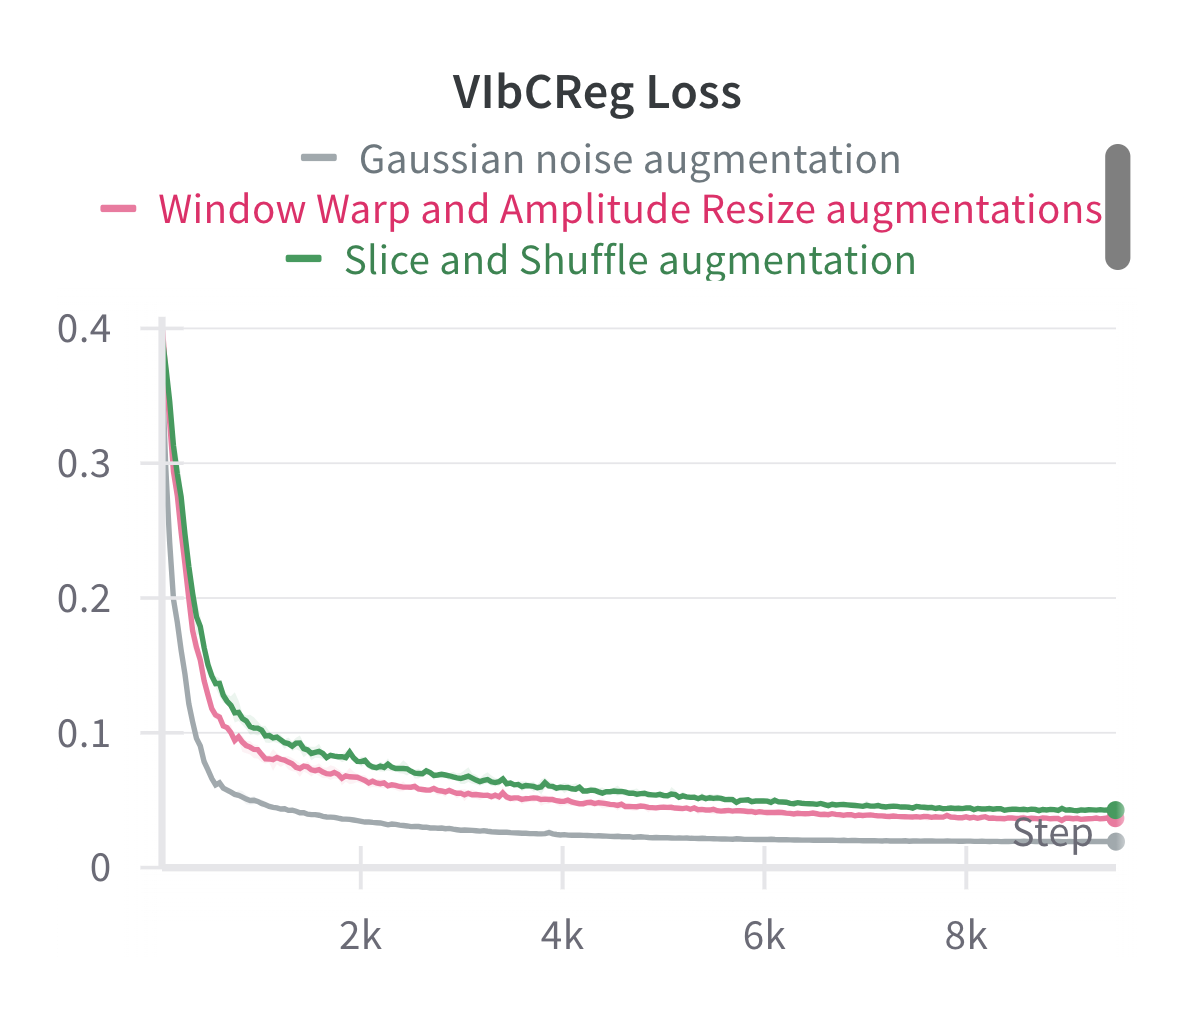
\includegraphics[width=\textwidth]{vib_loss_Uwave.png}
    \end{minipage}
    \caption{SSL loss during training on UWaveGestureLibraryAll. Averaged across four runs.}
    \label{fig:SSL_loss_UWave}
\end{figure}

The relatively straightforward minimization of the losses might be attributed to the fact that the gaussian augmentation affects the samples in a predictable way. Additionally, we note that the VIbCReg loss declines more rapidly than Barlow Twins across all datasets. \newline

Previously, in figure \ref{fig:Mean_probe}, we observed that Gaussian augmentation typically resulted in lower probe accuracy than warp and slice. In figure \ref{fig:Vibcreg_loss_knn_accuracy} we see that, for datasets where probe accuracy increased significantly, the augmentations that result in a more challenging SSL loss typically has higher downstream classification accuracy. Furthermore, we observe relatively stable patterns for specific augmentations, suggesting their significant impact on probe accuracy compared to variation in SSL loss.\newline

\begin{figure}[h]
    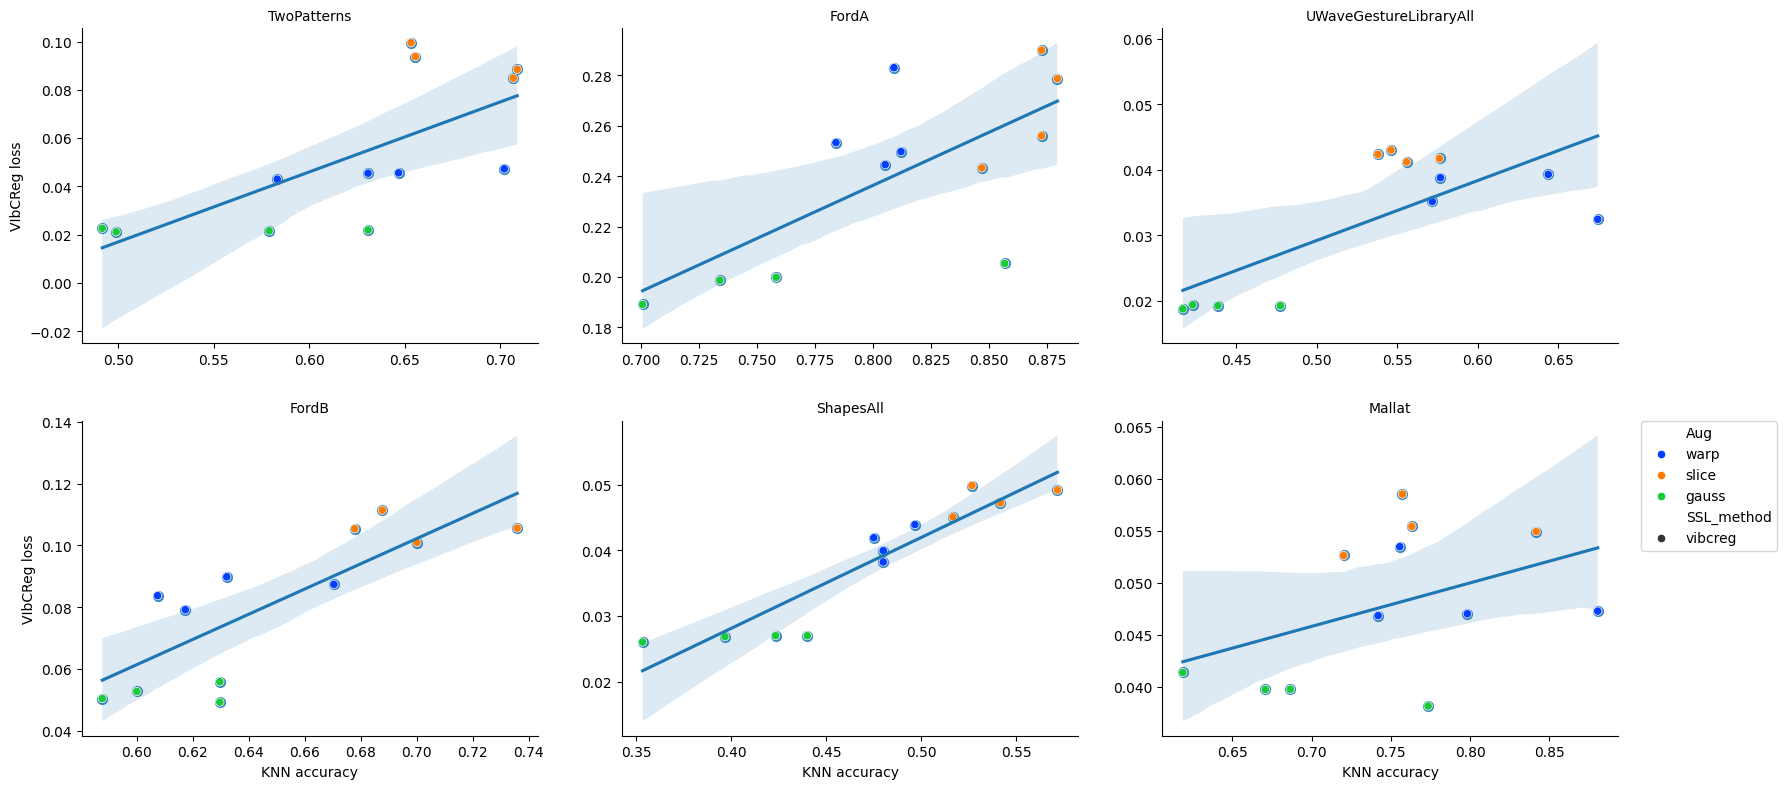
\includegraphics[scale=0.30]{Vibcreg_loss_knn_accuracy.png}
    \centering  
    \caption{KNN accuracy plotted against VIbCReg loss. Each point correspond to a single run of the model. Similar tendency is shown for Barlow Twins.}
    \label{fig:Vibcreg_loss_knn_accuracy}
\end{figure}

Reconstruction losses during training are consistently minimized across models and augmentations, with augmented reconstruction loss slightly higher in models utilizing Slice and Shuffle. Differences in VQ loss primarily stem from the codebook loss, with VIbCReg consistently exhibiting more effective minimization than Barlow Twins. Gaussian augmentation present the easiest minimization challenge, followed by Window Warp and Slice and Shuffle.\newline

Both VIbCReg and Barlow Twins, when coupled with Gaussian augmentation, consistently perform comparably to the naive VQVAE in terms of VQ loss during training. The minimization of the codebook loss indicates that the encoder is properly aligned with the discrete latent codes. We hypothesize that when the SSL loss is not properly minimized, the encoder must adjust its weights more throughout training which keeps the encoder outputs and the discrete codes from aligning completely.

\section{Stage 2}
The generative quality of our models is assessed using FID, IS, and CAS, with all results presented in this section. However, it's important to note that for datasets with limited samples or few samples per class, the generative scores should be interpreted cautiously. Both the classifier and evaluation metrics rely on a sufficient number of samples to ensure reliability. Therefore, visual inspection is prioritized for such cases.


\subsection{FID and IS}

Tables \ref{tab:FID_IS_best} and \ref{tab:FID_IS_mean} present the top 1 and mean scores across the four runs for both FID and IS. Analysis of the tables reveals that our model achieves higher IS scores for 12 out of 13 datasets and lower FID scores for 10 out of 13 datasets in both mean and top 1.\newline

\begin{table}[H]
    \title{Top 1 FID and IS}
    \centering
    \begin{adjustbox}{width=\textwidth}
     \begin{tabular}{lcc|cc|cc|cc|cc|cc|cc} % 15 cols, 1 for dataset, 14 for svm/knn across models (7 models)
        \toprule
        \multirow{4}{*}{\textbf{Dataset}} & \multicolumn{2}{c}{\textbf{Baseline}} & \multicolumn{12}{c}{\textbf{SSL Method}} \\
                                            \cmidrule(lr){2-3} \cmidrule(lr){4-15}
                                          & \multicolumn{2}{c}{Regular}           & \multicolumn{6}{c}{Barlow Twins}                                                 &  \multicolumn{6}{c}{VIbCReg} \\
                                          \cmidrule(lr){2-3} \cmidrule(lr){4-9} \cmidrule(lr){10-15}
                                          &   \multicolumn{2}{c}{None}            & \multicolumn{2}{c}{Warp}  & \multicolumn{2}{c}{Slice} & \multicolumn{2}{c}{Gauss} & \multicolumn{2}{c}{Warp} & \multicolumn{2}{c}{Slice} & \multicolumn{2}{c}{Gauss} \\
                                          \cmidrule(lr){2-3} \cmidrule(lr){4-5} \cmidrule(lr){6-7} \cmidrule(lr){8-9} \cmidrule(lr){10-11} \cmidrule(lr){12-13}\cmidrule(lr){14-15}
                                          & FID$\downarrow$ & IS$\uparrow $                             & FID$\downarrow$ & IS$\uparrow$                  & FID$\downarrow$ & IS$\uparrow$                & FID$\downarrow$ & IS$\uparrow$                 & FID$\downarrow$ & IS$\uparrow$                 & FID$\downarrow$ & IS $\uparrow$                 & FID$\downarrow$ & IS$\uparrow$   \\
        \midrule
        FordA                   & 2.59 & 1.30 & 1.93 & \textbf{1.51} & 2.13 & 1.48 & 1.80 & \textbf{1.51} & 2.83 & 1.38 & 2.50 & 1.43 & \textbf{1.66} & 1.41 \\
        ElectricDevices         & 12.05 & 3.97 & 11.82 & 4.20 & \textbf{8.91} & 4.07 & 9.89 & 3.86 & 12.38 & \textbf{4.23} & 11.08 & 3.94 & 13.96 & 3.71 \\
        StarLightCurves         & \textbf{0.74} & 1.99 & 0.89 & \textbf{2.43} & 1.50 & 2.36 & 0.75 & 2.39 & 0.92 & 2.39 & 0.85 & \textbf{2.40} & 0.79 & 2.26 \\
        Wafer                   & 5.27 & \textbf{1.39} & 3.31 & 1.29 & 3.82 & \textbf{1.26} & 2.77 & 1.35 & 3.33 & 1.29 & 3.60 & 1.30 & \textbf{2.52} & 1.34 \\
        ECG5000                 & 1.56 & 2.01 & 2.43 & 2.02 & 2.27 & 2.00 & 2.15 & 2.02 & 2.15 & \textbf{2.03} & 2.21 & 2.00 & \textbf{1.52} & 2.02 \\
        TwoPatterns             & 3.63 & 2.47 & 3.59 & 2.65 & 2.74 & 2.73 & \textbf{2.24} & 2.70 & 3.45 & 2.64 & 2.90 & 2.70 & \textbf{2.19} & \textbf{2.77} \\
        UWaveGestureLibraryAll  & 8.16 & 2.24 & 6.45 & 2.94 & \textbf{6.26} & \textbf{3.13} & 7.31 & 2.79 & 6.52 & 2.99 & 6.33 & 3.06 & 7.09 & 2.79 \\
        FordB                   & 2.92 & 1.52 & 2.10 & 1.52 & 2.44 & 1.61 & 1.93 & \textbf{1.67} & 1.76 & 1.65  & 2.12 & 1.64 & \textbf{1.66} & 1.52 \\
        ShapesAll               & \textbf{21.35} & 4.32 & 35.89 & \textbf{5.22} & 29.61 & 5.16 & 27.91 & 4.83 & 30.03 & 4.95 & 31.59 & 4.92 & 27.20 & 4.94 \\
        SonyAIBORobotSurface1   & 18.21 & 1.27 & 26.20 & 1.32 & 28.90 & 1.28 & 21.63 & 1.32 & 21.98 & 1.36 & 25.20 & 1.38 & \textbf{15.73} & \textbf{1.55} \\
        SonyAIBORobotSurface2   & 3.85 & 1.69 & 2.50 & 1.82 & 3.34 & 1.79 & \textbf{0.82} & 1.82 & 2.61 & 1.81 & 2.75 & 1.83 & 1.24 & \textbf{1.84} \\
        Symbols                  & 8.50 & 2.43 & 5.86 & 3.20 & 7.39 & 2.82 & \textbf{4.25} & \textbf{3.50} & 6.78 & 3.39 & 7.21 & 3.23 & 8.21 & 3.30 \\
        Mallat                   & \textbf{1.31} & 3.41 & 2.01 & 3.67 & 2.24 & 3.72 & 1.85 & 3.66 & 1.87 & 3.34 & 2.30 & 3.05 & \textbf{1.31} & \textbf{3.92} \\
        \bottomrule
    \end{tabular}
    \end{adjustbox}
    \caption{Summary of FID and IS scores by SSL Method and Augmentation. Best achieved results are highlighted in bold}
    \label{tab:FID_IS_best}
\end{table}


\begin{table}[h]
    \centering
    \title{Mean FID and IS}
    \begin{adjustbox}{width=\textwidth}
     \begin{tabular}{lcc|cc|cc|cc|cc|cc|cc} % 15 cols, 1 for dataset, 14 for svm/knn across models (7 models)
        \toprule
        \multirow{4}{*}{\textbf{Dataset}} & \multicolumn{2}{c}{\textbf{Baseline}} & \multicolumn{12}{c}{\textbf{SSL Method}} \\
                                            \cmidrule(lr){2-3} \cmidrule(lr){4-15}
                                          & \multicolumn{2}{c}{Regular}           & \multicolumn{6}{c}{Barlow Twins}                                                 &  \multicolumn{6}{c}{VIbCReg} \\
                                          \cmidrule(lr){2-3} \cmidrule(lr){4-9} \cmidrule(lr){10-15}
                                          &   \multicolumn{2}{c}{None}            & \multicolumn{2}{c}{Warp}  & \multicolumn{2}{c}{Slice} & \multicolumn{2}{c}{Gauss} & \multicolumn{2}{c}{Warp} & \multicolumn{2}{c}{Slice} & \multicolumn{2}{c}{Gauss} \\
                                          \cmidrule(lr){2-3} \cmidrule(lr){4-5} \cmidrule(lr){6-7} \cmidrule(lr){8-9} \cmidrule(lr){10-11} \cmidrule(lr){12-13}\cmidrule(lr){14-15}
                                          & FID$\downarrow$ & IS$\uparrow $                             & FID$\downarrow$ & IS$\uparrow$                  & FID$\downarrow$ & IS$\uparrow$                & FID$\downarrow$ & IS$\uparrow$                 & FID$\downarrow$ & IS$\uparrow$                 & FID$\downarrow$ & IS $\uparrow$                 & FID$\downarrow$ & IS$\uparrow$   \\
        \midrule
        FordA                   & 5.15 & 1.16 & 2.59 & 1.41 & 2.36 &\textbf{ 1.45} & \textbf{2.28} & \textbf{1.45} & 3.01 & 1.34 & 2.90 & 1.41 & 3.73 & 1.29 \\
        ElectricDevices         & 13.48 & 3.75 & 16.51 & 3.95 & \textbf{10.20} & 3.93 & 11.54 & 3.75 & 13.99 & \textbf{4.17} & 11.82 & 3.85 & 15.20 & 3.55 \\
        StarLightCurves         & \textbf{1.01} & 1.93 & 1.29 & 2.35 & 1.91 & 2.32 & 1.08 & 2.25 & 1.07 & 2.35 & 1.19 & \textbf{2.36} & 1.05 & 2.22 \\
        Wafer                   & 5.72 & \textbf{1.33} & 3.70 & 1.25 & 4.20 & 1.24 & 2.85 & 1.31 & 3.67 & 1.26 & 3.86 & 1.26 & \textbf{2.84} & 1.31 \\
        ECG5000                 & \textbf{1.62} & 1.94 & 2.61 & \textbf{2.00} & 2.56 & 1.98 & 2.47 & \textbf{2.00} & 2.60 & 1.99 & 2.39 & \textbf{2.00} & 1.76 & 1.99 \\
        TwoPatterns             & 4.04 & 2.41 & 4.00 & 2.54 & 2.96 & 2.66 & \textbf{2.44} & \textbf{2.67} & 4.05 & 2.56 & 3.15 & 2.66 & 2.62 & \textbf{2.67} \\
        UWaveGestureLibraryAll  & 8.48 & 2.13 & 6.77 & 2.86 & 6.64 & 2.96 & 7.35 & 2.73 & 6.80 & 2.91 & \textbf{6.49} & \textbf{2.99} & 7.34 & 2.72 \\
        FordB                   & 4.05 & 1.28 & 2.66 & 1.48 & 3.49 & 1.50 & 2.88 & \textbf{1.52} & \textbf{2.49} & 1.48 & 3.07 & 1.51 & 3.04 & 1.31 \\
        ShapesAll               & \textbf{27.64} & 4.22 & 38.22 & 5.07 & 32.54 & \textbf{5.04} & 32.25 & 4.56 & 36.59 & 4.72 & 35.79 & 4.76 & 31.56 & 4.71 \\
        SonyAIBORobotSurface1   & 23.71 & 1.20 & 30.65 & 1.22 & 31.97 & 1.21 & 25.29 & 1.28 & 26.11 & 1.32 & 28.20 & 1.32 & \textbf{18.61} & \textbf{1.44} \\
        SonyAIBORobotSurface2   & 5.42 & 1.62 & 3.35 & 1.77 & 4.41 & 1.74 & \textbf{1.78} & \textbf{1.81} & 4.43 & 1.74 & 3.32 & 1.79 & 2.36 & 1.79 \\
        Symbols                 & 13.62 & 1.99 & 9.78 & 2.92 & 9.78 & 2.67 & 8.61 & 3.14 & 8.84 & 3.20 & 9.74 & 3.03 & \textbf{8.58} & \textbf{3.24} \\
        Mallat                  & 2.09 & 3.01 & 2.54 & 3.29 & 3.68 & 2.94 & 2.12 & 3.53 & 2.11 & 3.18 & 2.40 & 2.96 & \textbf{1.65} & \textbf{3.72} \\
        \bottomrule
    \end{tabular}
    \end{adjustbox}
    \caption{Summary of FID and IS scores by SSL Method and Augmentation. Best mean achieved FID and IS are highlighted in bold}
    \label{tab:FID_IS_mean}
\end{table}

In Figure \ref{fig:mean_gen_scores}, an overview of the results highlights that both Barlow Twins and VIbCReg generally yield better samples than the naive VQVAE in terms of FID and IS. There is a difference in VIbCReg and Barlow Twins, in that VIbCReg is more robust to the particular choice of augmentation, which is particularly evident when looking at the Slice and Shuffle augmentation. Furthermore, the use of Gaussian augmentation leads to the most significant improvements across most datasets. The high IS scores suggest that NC-VQVAE captures the conditional distributions more accurately than the naive VQVAE across many datasets. The improved FID scores indicates that the synthetic samples more closely resemble the test data. This will be explored further in Section \ref{section:Visual inspection}. The moderate decrease in FID, compared to the increase in IS, could indicate that the generated samples does not generalize too well to the test data. However, the discrete latent representations from NC-VQVAE offer additional class-specific information, as evidenced by the improved downstream classification accuracy observed in stage 1. This supplementary class-specific information appears to assist the prior learning process in capturing class conditional distributions.

\begin{figure}[h]
    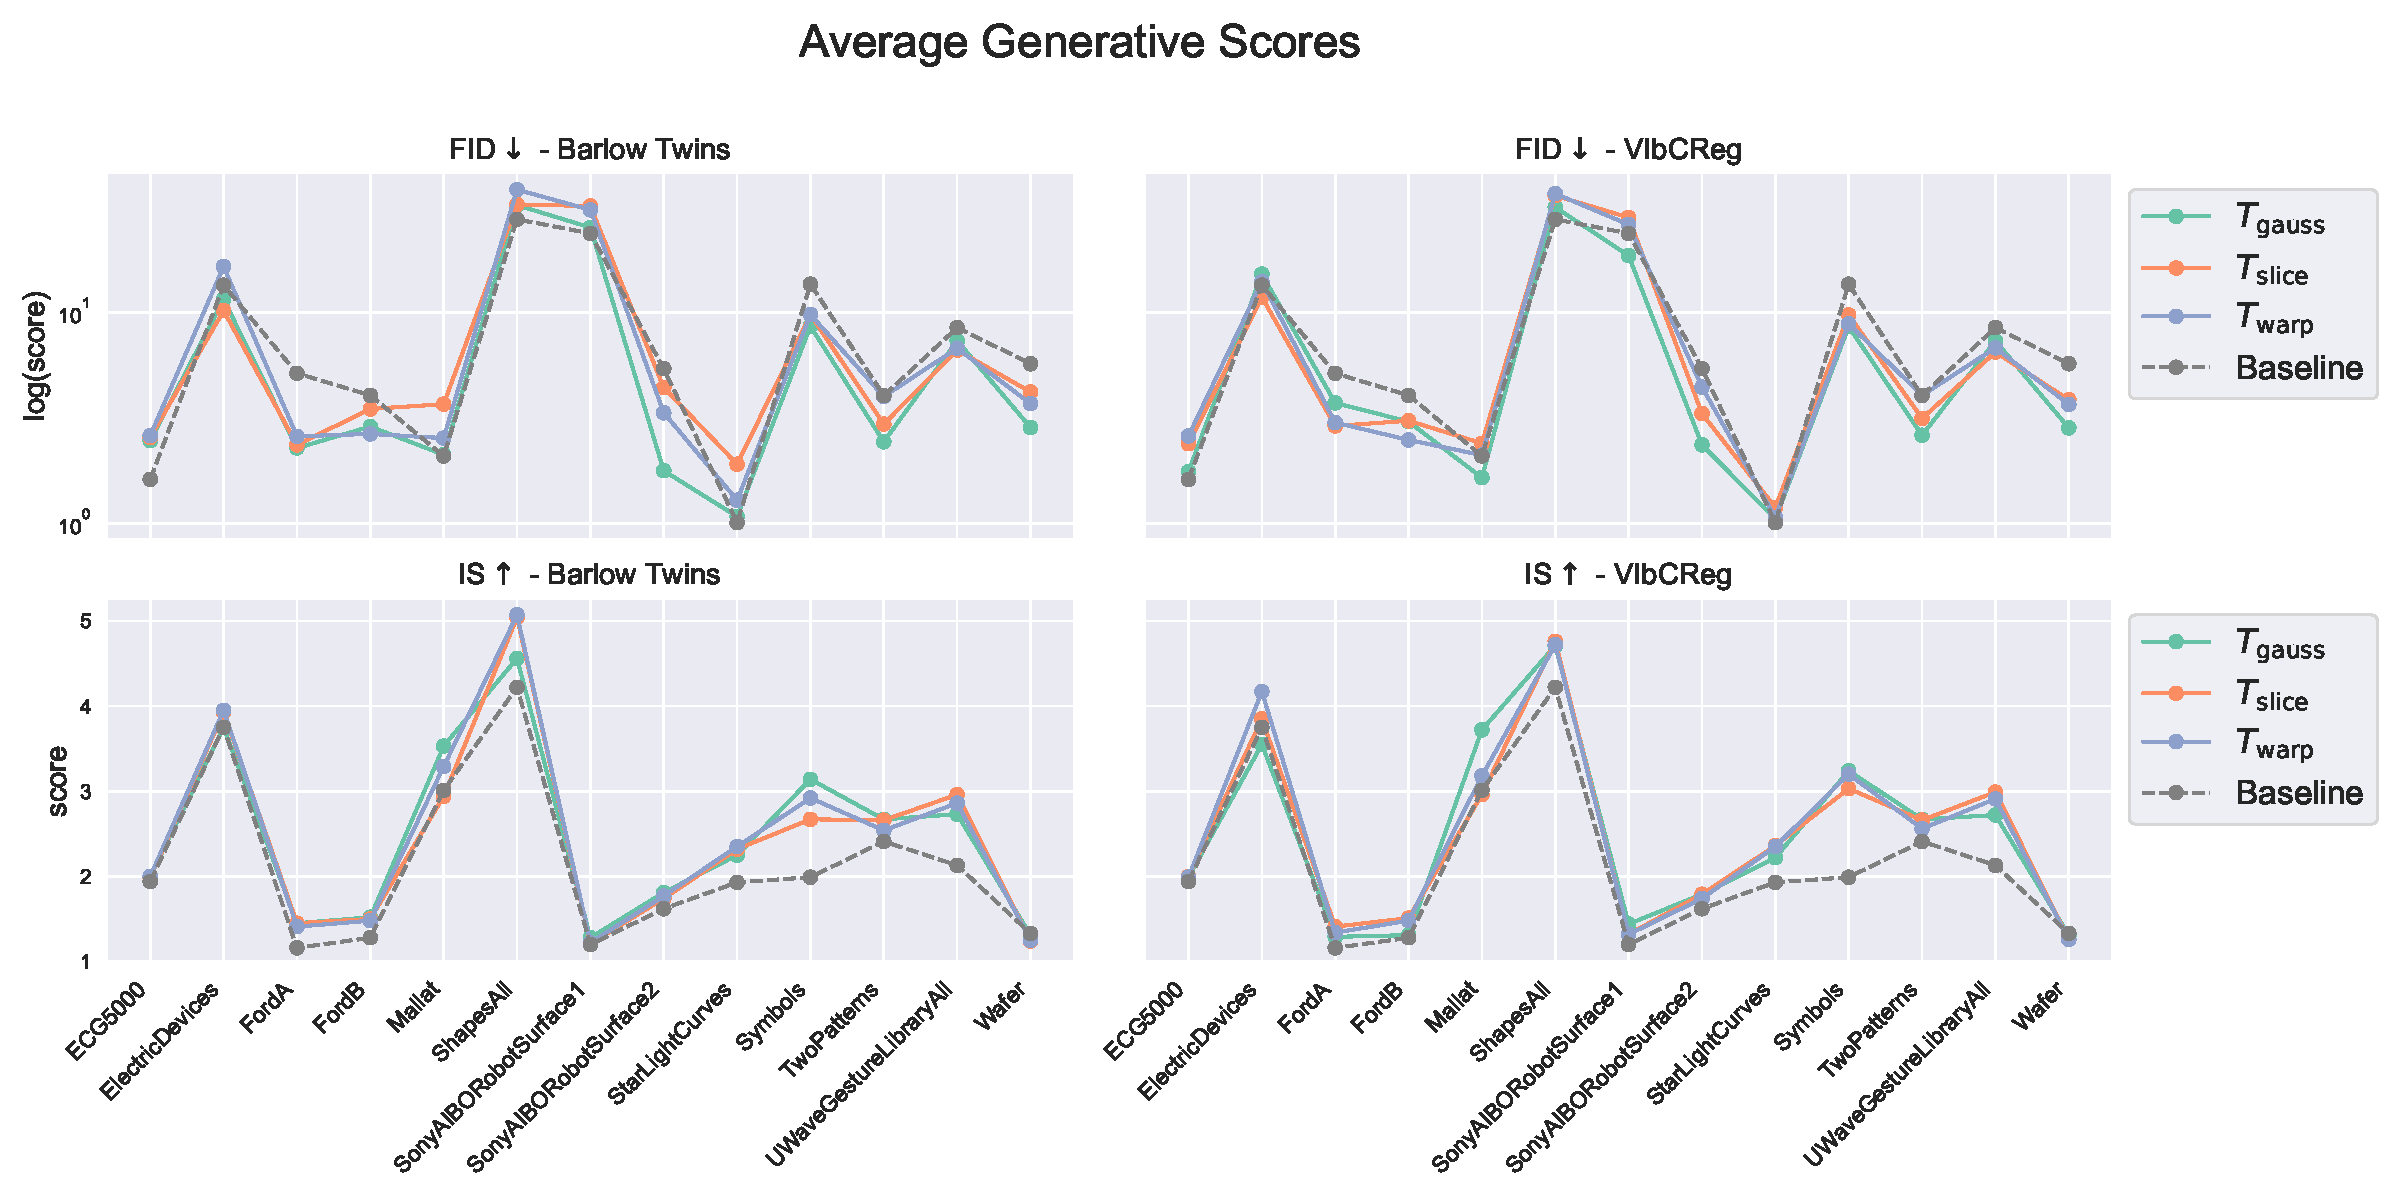
\includegraphics[scale=0.35]{gen_scores.pdf}
    \centering  
    \caption{Mean FID and IS scores for Barlow Twins and VIbCReg VQVAE. FID is plotted on a log scale because of the large difference in values across datasets.}
    \label{fig:mean_gen_scores}
\end{figure}

It's important to note that the FID and IS scores are calculated using the SupervisedFCN, which is trained on the UCR Archive. Consequently, there may be a bias towards samples that mimic the training data.


\subsection{CAS}

We present the mean CAS for all models across datasets in Table \ref{tab:mean_cas}.

\begin{table}[H]
    \centering
    \title{Mean CAS}
    \begin{adjustbox}{width=\textwidth}
    \begin{tabular}{lc|c|c|c|c|c|c} % 8 cols, 1 for dataset, 7 for val_recons across models (7 models)
        \toprule
        \multirow{3}{*}{\textbf{Dataset}} & \multicolumn{1}{c}{\textbf{Baseline}} & \multicolumn{6}{c}{\textbf{SSL Method}} \\
                                         \cmidrule(lr){3-8}
                                          & \multicolumn{1}{c}{Regular}           & \multicolumn{3}{c}{Barlow Twins}    &  \multicolumn{3}{c}{VIbCReg} \\
                                                                                   \cmidrule(lr){3-5}                    \cmidrule(lr){6-8}
                                          &   None                                & Warp  & Slice & Gauss               & Warp & Slice & Gauss \\
                            
        \midrule
        FordA                   & 0.864 & 0.884 & \textbf{0.902} & 0.878 & 0.864 & 0.895 & 0.870 \\
        ElectricDevices         & 0.614 & 0.588 & 0.607 & 0.599 & \textbf{0.618} & 0.610 & 0.594 \\
        StarLightCurves         & 0.960 & 0.953 & 0.955 & \textbf{0.965} & 0.962 & 0.954 & 0.964 \\
        Wafer                   & 0.976 & 0.977 & 0.978 & 0.968 & 0.979 & 0.976 & \textbf{0.984} \\
        ECG5000                 & 0.866 & 0.881 & 0.863 & 0.880 & 0.877 & 0.892 & \textbf{0.910} \\
        TwoPatterns             & 0.808 & 0.770 & 0.788 & \textbf{0.847} & 0.715 & 0.781 & 0.846 \\
        UWaveGestureLibraryAll  & 0.333 & 0.300 & 0.367 & 0.313 & 0.360 & \textbf{0.401} & 0.383 \\
        FordB                   & 0.725 & 0.748 & \textbf{0.756} & 0.741 & 0.750 & 0.738 & 0.750 \\
        ShapesAll               & 0.361 & 0.344 & 0.329 & \textbf{0.420 }& 0.379 & 0.367 & 0.404 \\
        SonyAIBORobotSurface1   & 0.975 & 0.933 & 0.957 & 0.979 & 0.982 & 0.976 & \textbf{0.985} \\
        SonyAIBORobotSurface2   & 0.929 & 0.956 & 0.951 & 0.969 & 0.960 & \textbf{0.970} & 0.964 \\
        Symbols                 & 0.956 & 0.929 & 0.930 & 0.930 & 0.969 & \textbf{0.974} & 0.963 \\
        Mallat                  & 0.471 & 0.642 & 0.563 & 0.661 & 0.827 & 0.876 & \textbf{0.908} \\
        \bottomrule
    \end{tabular}
    \end{adjustbox}
    \caption{Mean CAS score across datasets. Results averaged across four runs.}
    \label{tab:mean_cas}
\end{table}

We observe that some configuration of NC-VQVAE outperform the naive VQVAE on all datasets. Additionally, VIbCReg with gaussian augmentation outperforms the baseline on 12 out of 13 datasets. Generally the difference in CAS is small for the different models, with the exception of Mallat, where VIbCReg with Gaussian augmentaion leads to an improvement of $0.437$ compared to baseline. This spesific case will be investigated further in Section \ref{section:Visual inspection}.

\begin{figure}[h]
    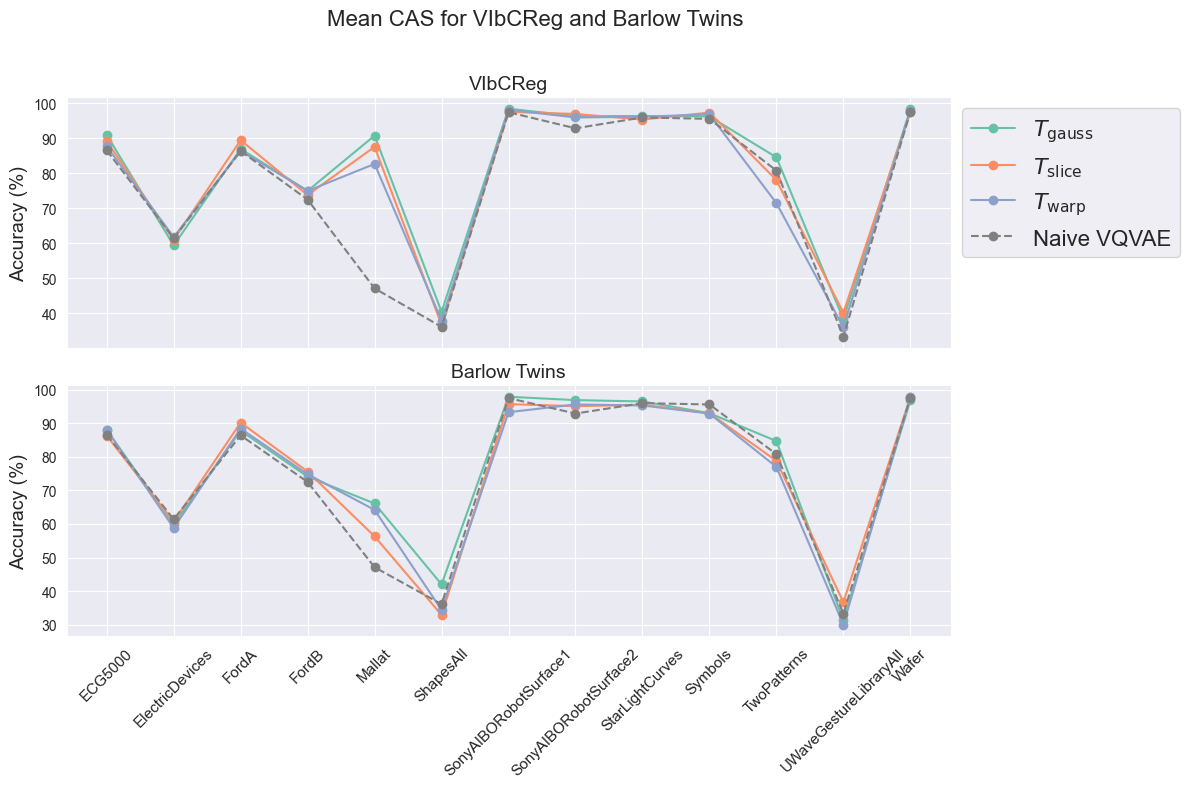
\includegraphics[scale=0.4]{Mean_CAS.png}
    \centering  
    \caption{Mean CAS across all datasets.}
    \label{fig:Mean_CAS}
\end{figure}


\subsection{Prior Loss}

In Figure \ref{fig:val_prior}, we illustrate the evolution of the validation prior loss during training. We observe that naive VQVAE outperforms all configurations of NC-VQVAE, and this pattern observed is representative for most datasets. The exception being SonyAIBORobotSurface1 and 2, where Barlow Twins with warp augmentation exhibits slightly better performance. These observations suggest that minimizing the validation prior loss does not necessarily correlate with improved generative scores.


\begin{figure}[h]
    \centering
    % \hfill
    \begin{minipage}[b]{0.32\textwidth}
        \centering
        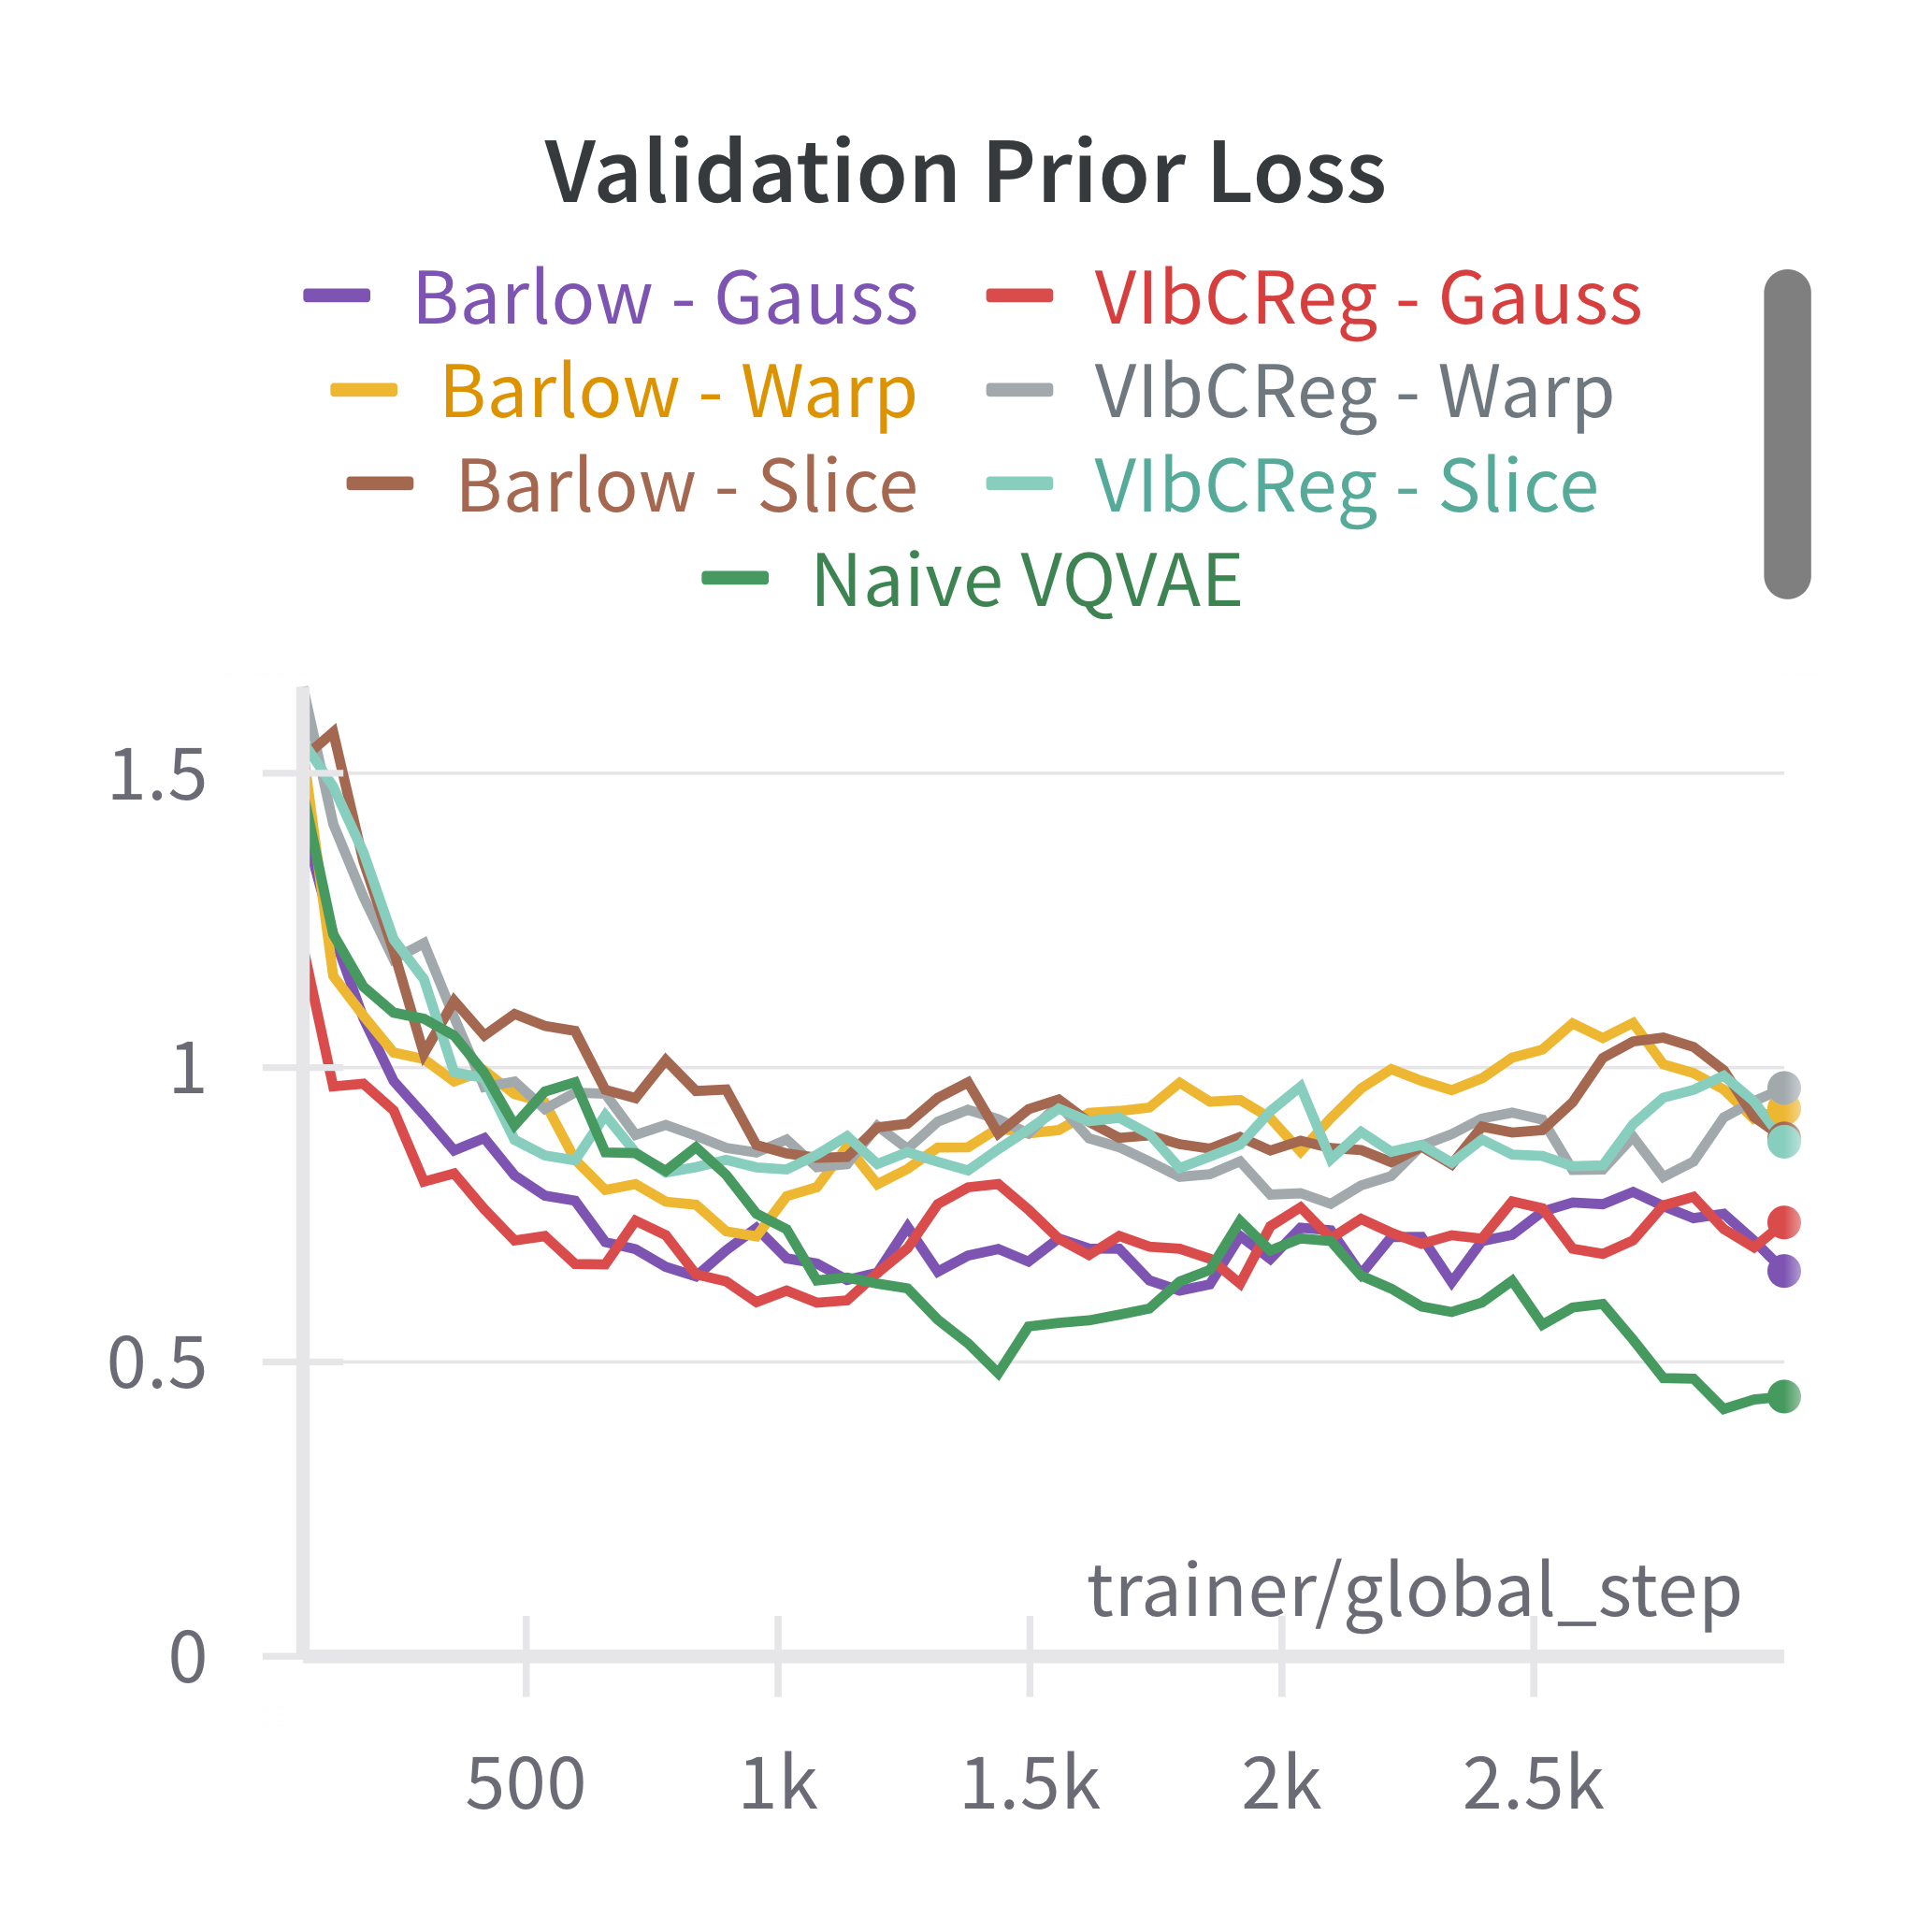
\includegraphics[width=\textwidth]{Val_prior_ShapesAll.png}
        \caption*{ShapesAll}
    \end{minipage}
    \begin{minipage}[b]{0.32\textwidth}
        \centering
        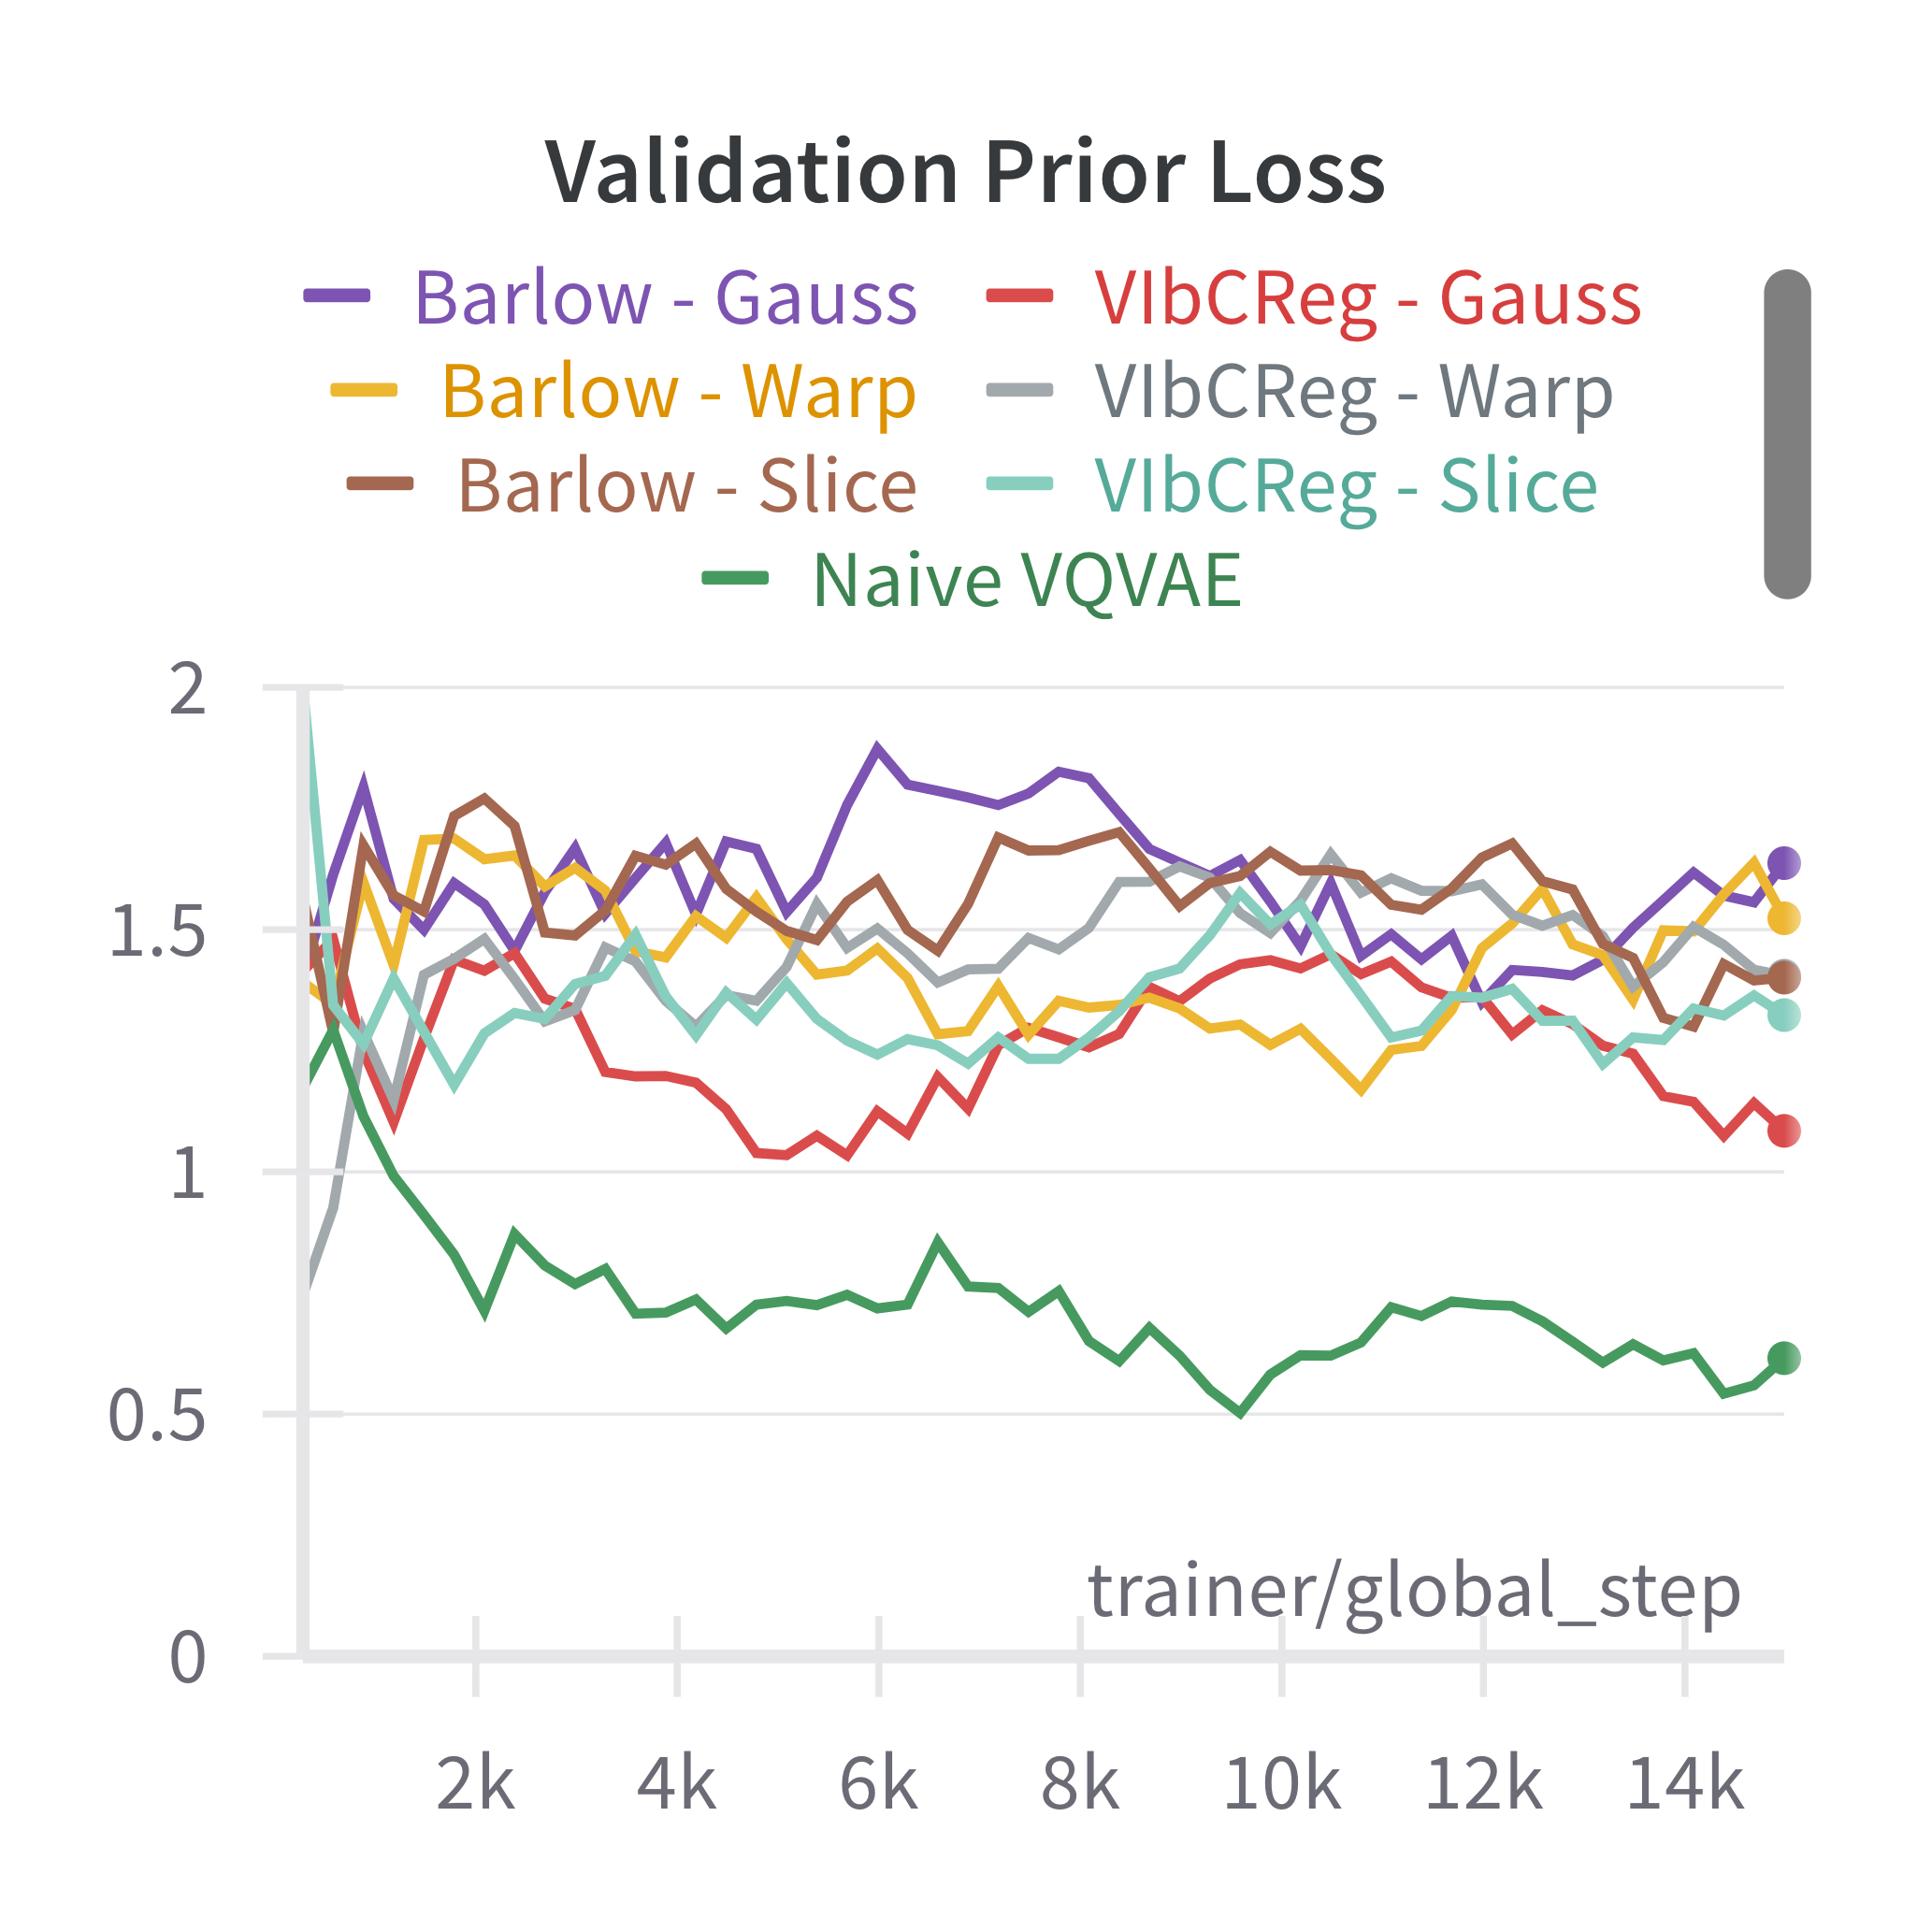
\includegraphics[width=\textwidth]{Val_prior_FordA.png}
        \caption*{FordA}
    \end{minipage}
    % \vspace{0.4cm}
    \begin{minipage}[b]{0.32\textwidth}
        \centering
        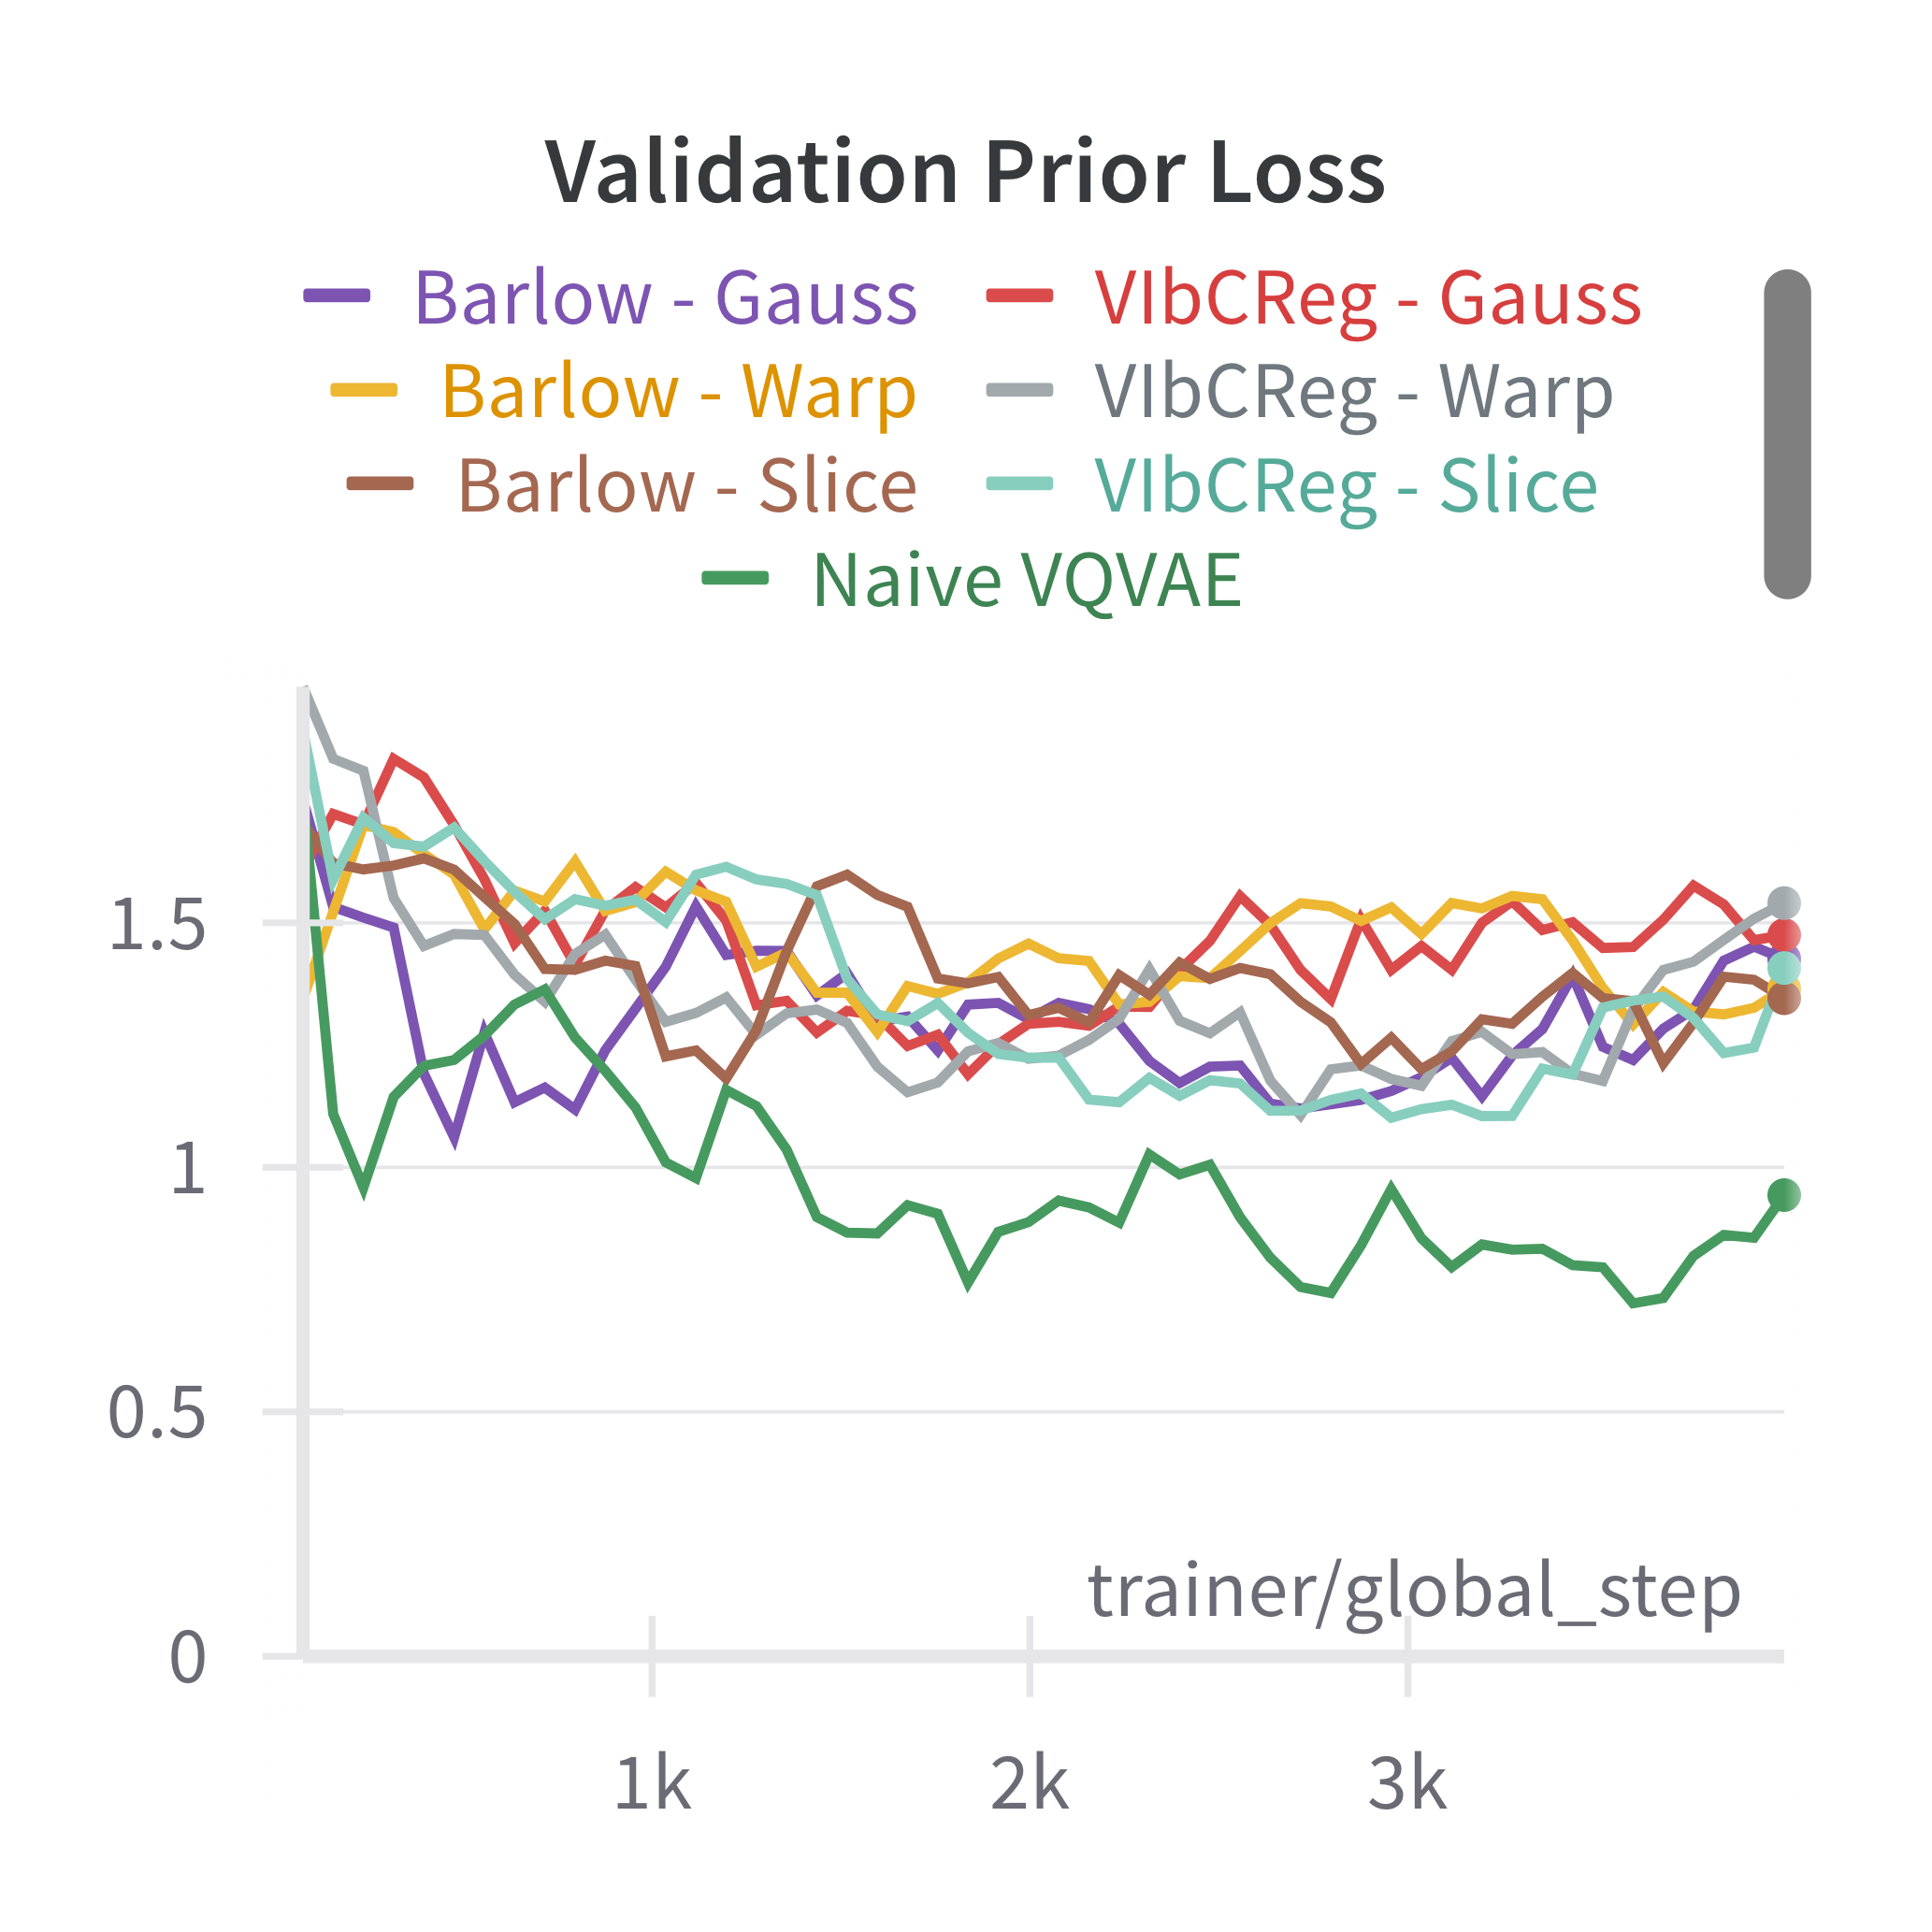
\includegraphics[width=\textwidth]{Val_prior_TwoPatterns.png}
        \caption*{TwoPatterns}
    \end{minipage}
    \caption{Validation prior loss during training for selected datasets. Averaged across all runs. Results averaged using exponential moving average with decay 0.7.}
    \label{fig:val_prior}
\end{figure}


\subsection{The influence of stage 1 on stage 2}

We aim to address research questions 3 and 4, which focus on how expressive representations influence the quality of synthetic samples and the role of augmentations. To explore this, we examine the relationship between probe accuracy and FID and IS metrics. Specifically, we focus on datasets where NC-VQVAE demonstrated a significant increase in probe accuracy, namely FordA, FordB, Mallat, ShapesAll, TwoPatterns, and UWaveGestureLibraryAll.\newline

In Figure \ref{fig:KNN_IS_Subset} and \ref{fig:KNN_FID_Subset}, we present scatterplots of KNN against FID and IS, respectively, along with the least square regression line. Similar trends are observed in the corresponding plots with SVM accuracy. 
From Figure \ref{fig:KNN_IS_Subset}, we observe a trend, where higher probe accuracy correlates with higher IS. Upon closer inspection, we see a pattern of the prominent effect of augmentations. For each specific augmentation, the correlation between KNN and IS is close to $0$. It appears that augmentations leading to higher KNN accuracy tend to result in higher IS scores, though the pattern is not consistent across all datasets. In Figure \ref{fig:KNN_FID_Subset}, we notice that the specific augmentation serves as a better indicator of FID score than KNN accuracy. Both figures also illustrate the sensitivity of model performance to initialization, particularly in terms of probe accuracy.\newline
\begin{figure}[h]
    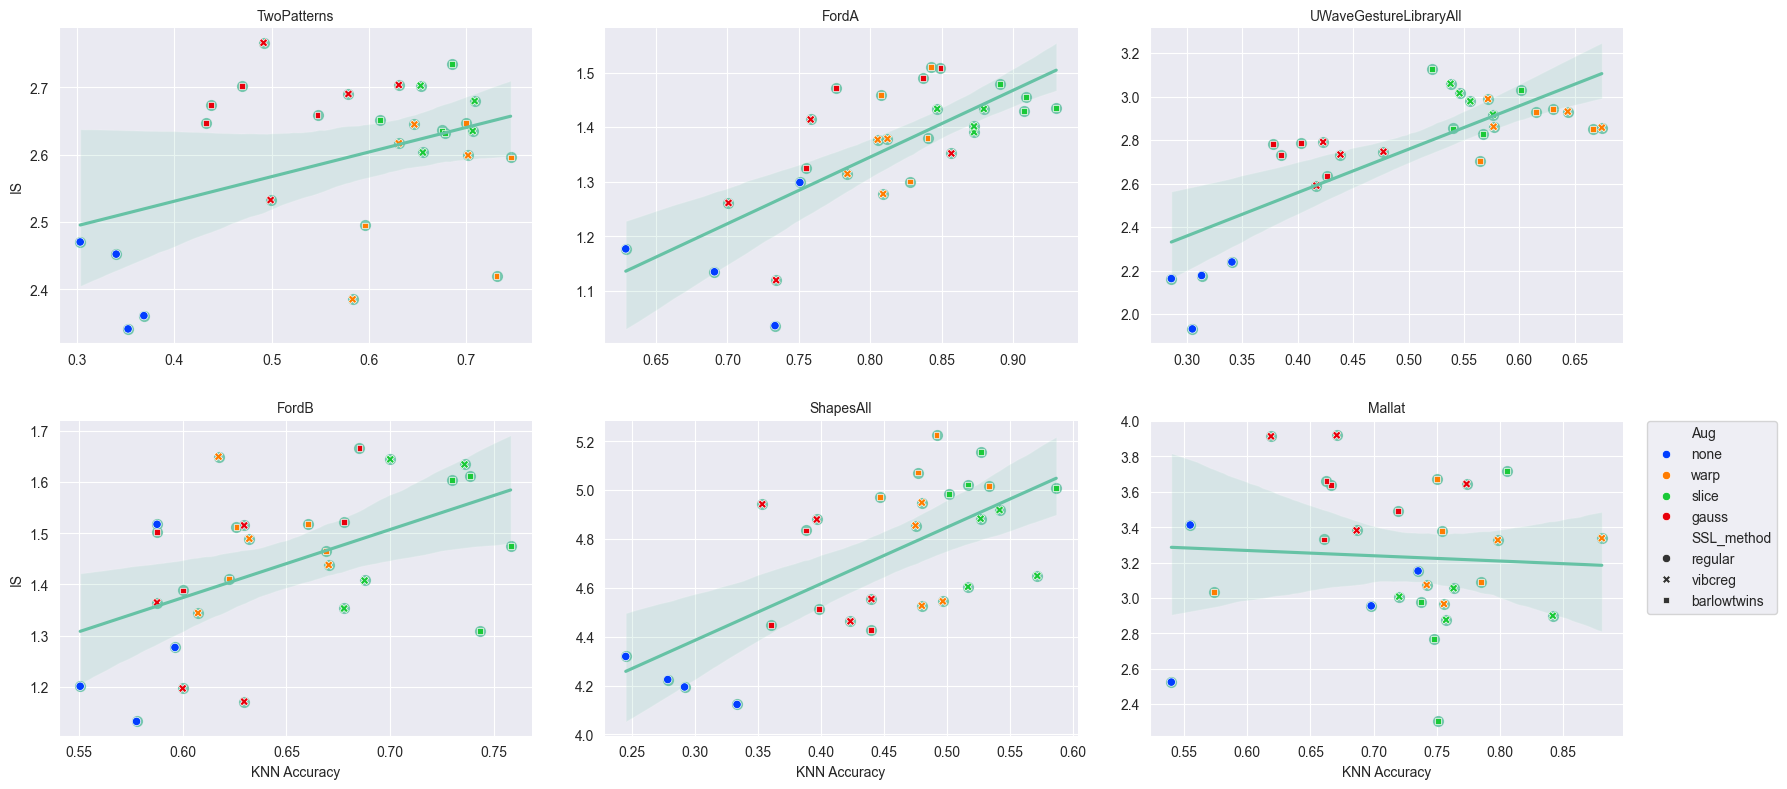
\includegraphics[scale=0.3]{KNN_IS_Subset.png}
    \centering  
    \caption{KNN plotted against Inception Score on the subset of datasets with significant improvement in probe accuracy.}
    \label{fig:KNN_IS_Subset}
\end{figure}

\begin{figure}[h]
    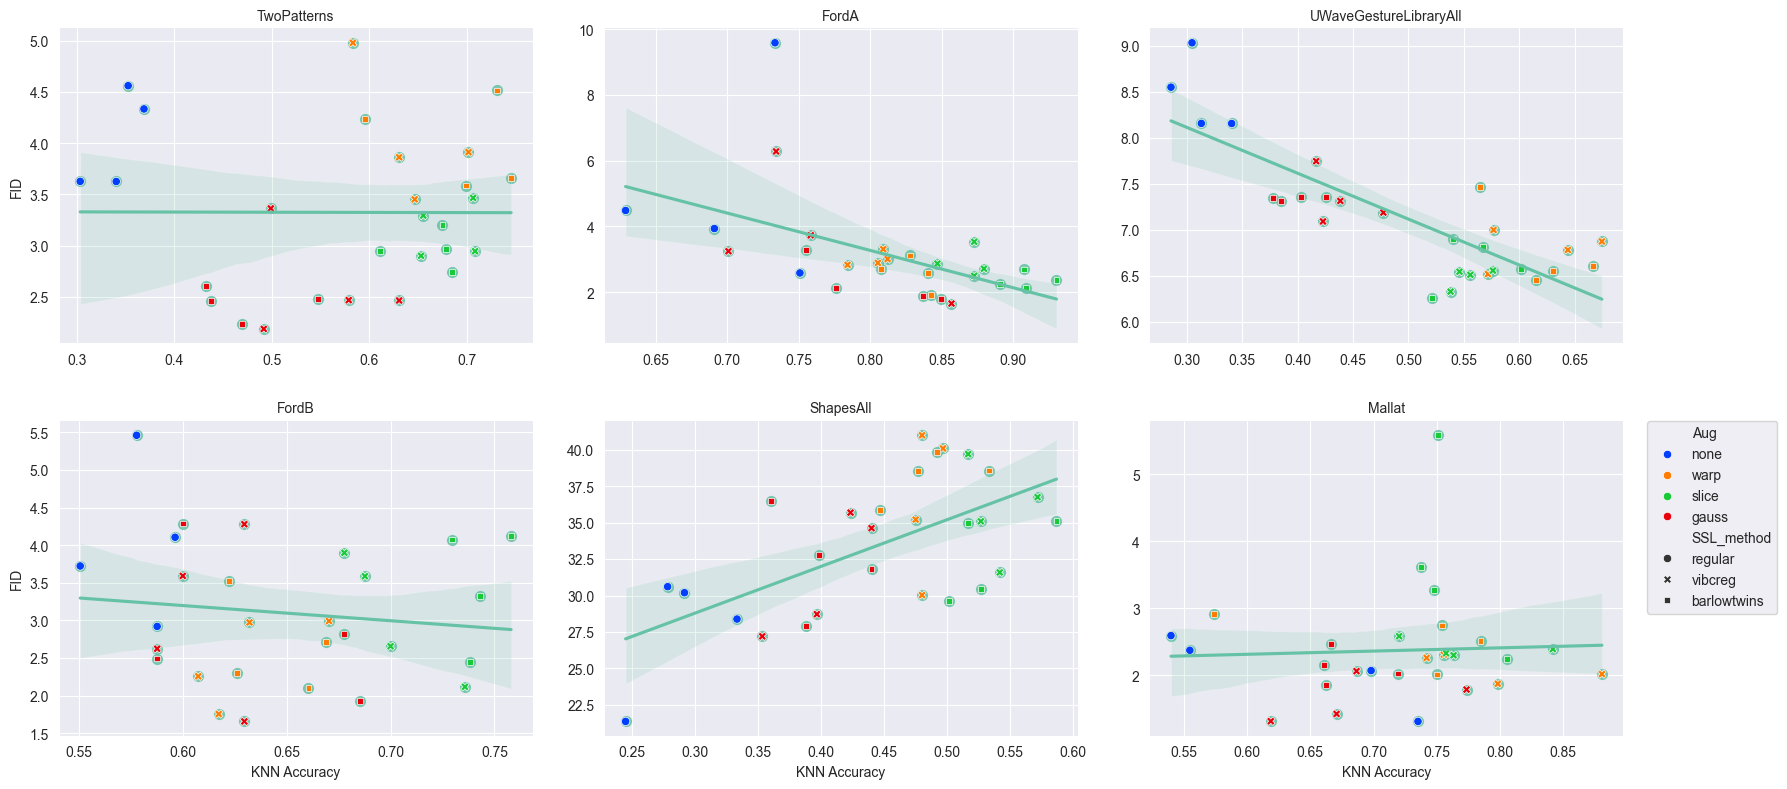
\includegraphics[scale=0.3]{KNN_FID_Subset.png}
    \centering  
    \caption{KNN plotted against Fréchet Inception Distance on the subset of datasets with significant improvement in probe accuracy.}
    \label{fig:KNN_FID_Subset}
\end{figure}



\subsection{Visual inspection}
\label{section:Visual inspection}
In the following we present generated samples from naive VQVAE and NC-VQVAE for selected datasets. The ground truth, both test and train, are additionally included in order to better make sense of the IS, FID and CAS scores. \newline

Some datasets, such as FordA and FordB, are poorly suited for this type of visual inspection, as illustrated previously in Figure \ref{fig:datasets}. As a result, the selection of datasets is primarily based on how well they lend themselves to this type of presentation. For each figure in the following sections, 50 samples are generated from each model. For the ground truth, we plot a subset of 50 randomly selected samples, or the entire set if the dataset contain less than 50 samples. For the datasets with complex distribution, or many classes, it is very difficult to visually asses the unconditional distribution. Thus, we mainly provide class conditional samples. We surprisingly only observe minor differences in the generated samples from NC-VQVAE trained with different augmentations.\newline

Typically naive VQVAE has more difficulty with capturing the global consistency of the samples when training samples are scarce and diverse, as seen on ShapesAll and Symbols. In contrast, our method will tend to overfit in these cases. The overfitting issue is most prominent in the class conditional distributions.

\subsubsection{ECG5000}

In Figure \ref{fig:Warp_ECG5000} we present generated samples from naive VQVAE and NC-VQVAE trained with Window Warp and Amplitude Resize augmentations on ECG5000.\newline


\begin{figure}[h]
    \centering
    % \hfill
    \begin{minipage}[b]{0.32\textwidth}
        \centering
        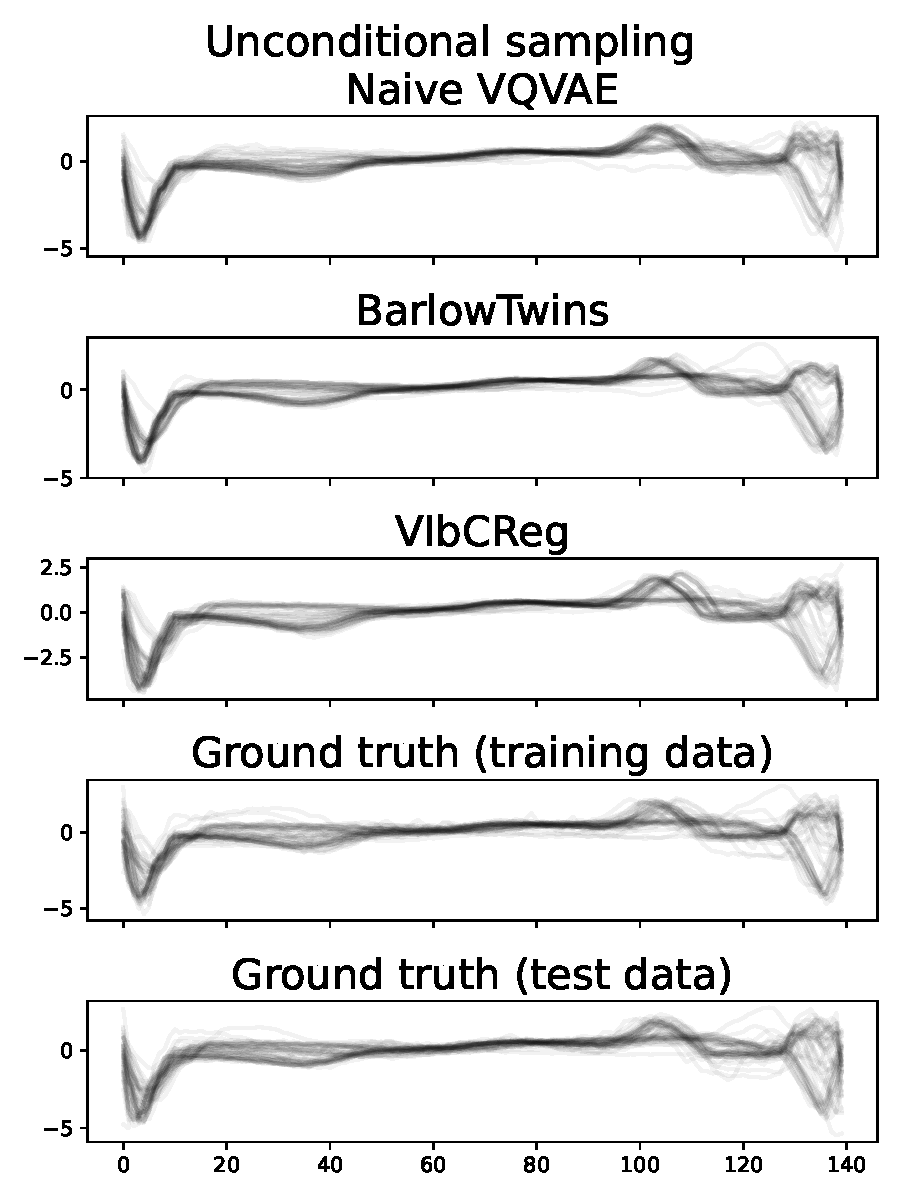
\includegraphics[width=\textwidth]{ECG5000-unconditional.pdf}
    \end{minipage}
    \begin{minipage}[b]{0.32\textwidth}
        \centering
        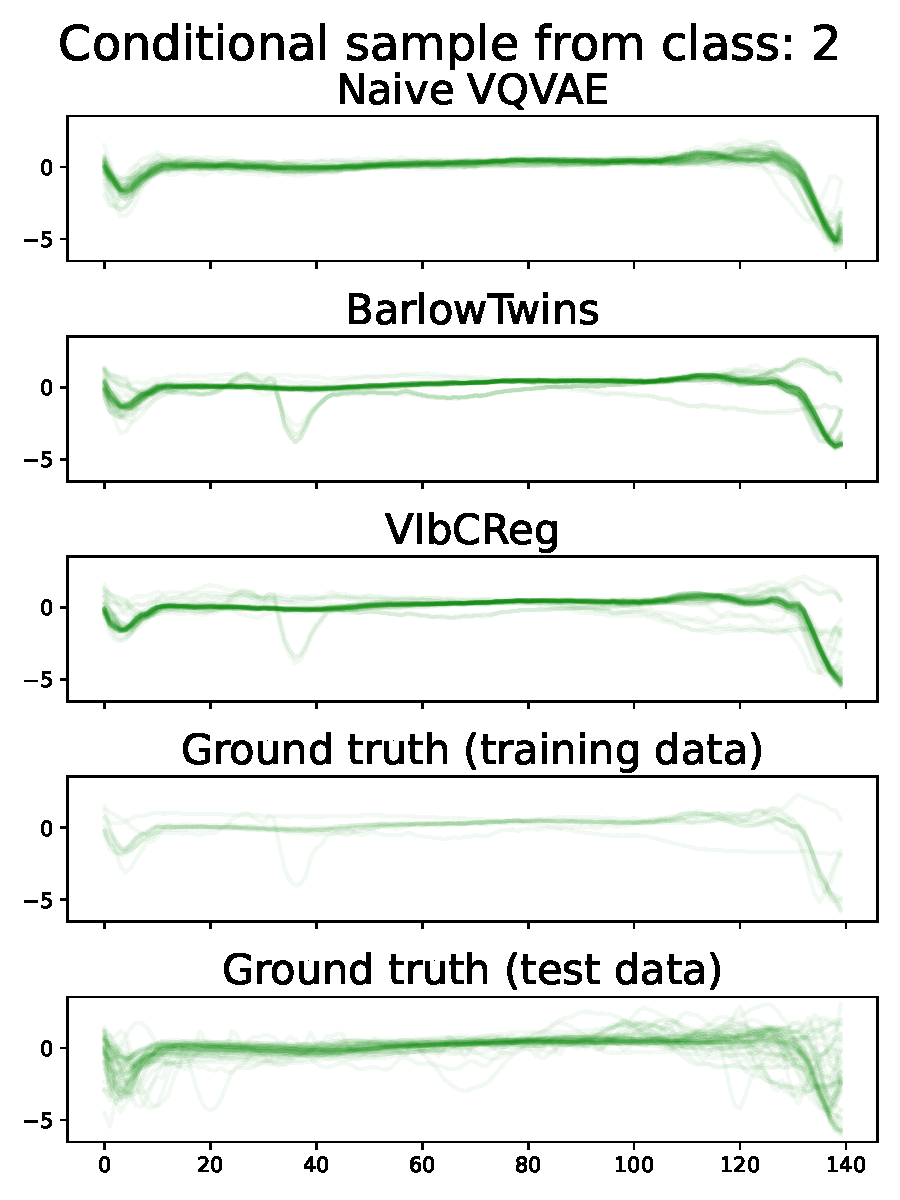
\includegraphics[width=\textwidth]{ECG5000-conditional-class2.pdf}
    \end{minipage}
    \begin{minipage}[b]{0.32\textwidth}
        \centering
        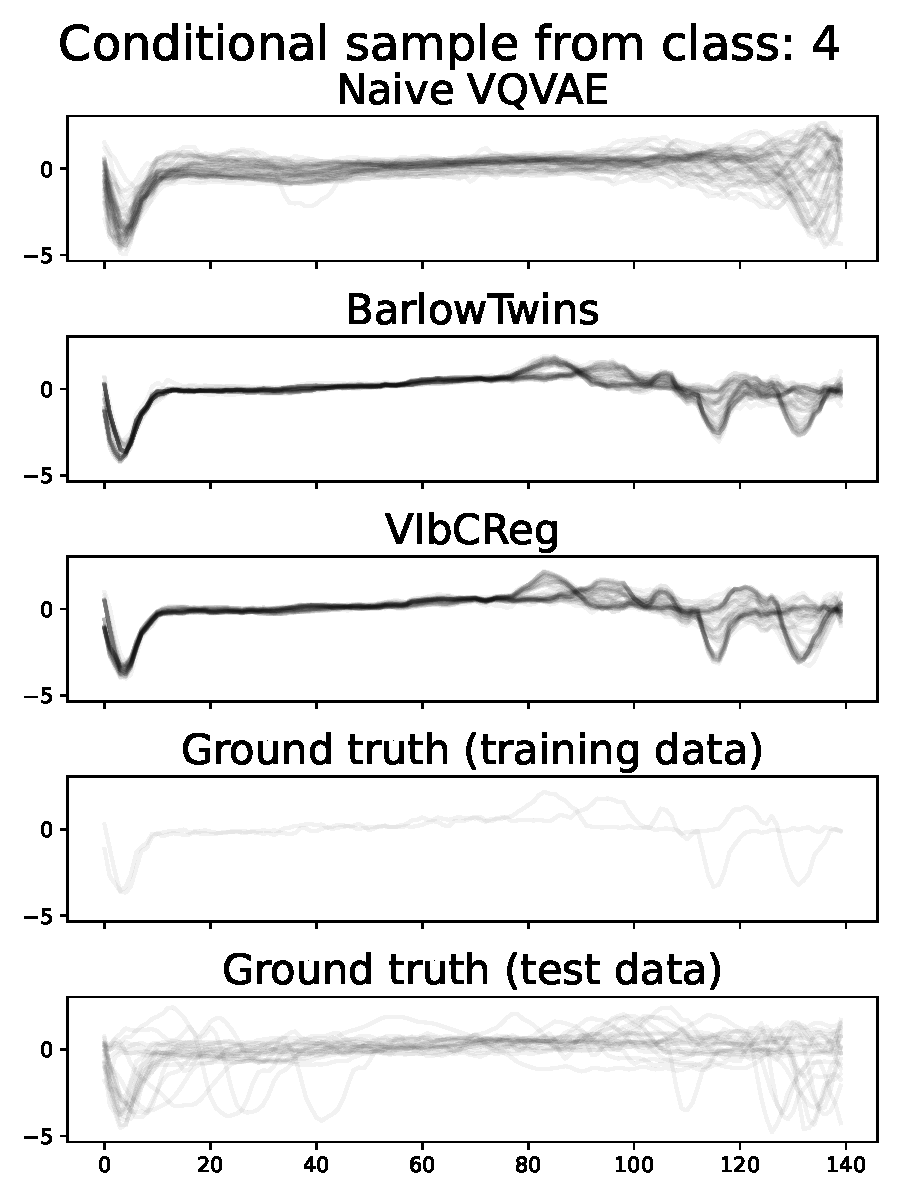
\includegraphics[width=\textwidth]{ECG5000-conditional-class4.pdf}
    \end{minipage}
    \caption{Dataset: ECG5000. Barlow and VIbCReg both trained with window warp and amplitude resize augmentations. 50 samples from each model.}
    \label{fig:Warp_ECG5000}
\end{figure}


We see some evidence that VIbCReg maintains more variability than Barlow Twins, while both have good mode coverage. In class 4, where the training data only consists of 2 samples, both Barlow Twins and VIbCReg catches the pattern, while producing some variation which resemble the training samples. The naive VQVAE samples does not capture this distribution, but when compared to the test data, it is more similar. This could explain the minor increase in CAS for NC-VQVAE. Looking at the unconditional sample, it is not evident why naive VQVAE performs better in terms of FID score than NC-VQVAE.


\subsubsection{Mallat}
Mallat is a simulated dataset, where the classes have very little variability and training and test distribution are almost indistinguishable, except for sample size. \newline

We observe that VIbCReg is superior in capturing the variability, compared to Barlow Twins and naive VQVAE. This is most evident in the first 300 timesteps of class 5 in Figure \ref{fig:Gaussian_Mallat}. Looking as class 7, we see Barlow Twins completely collapsing, essentially producing the same sample over and over. These figures explain the significant increase in CAS seen in Figure \ref{fig:Mean_CAS}, particularly for VIbCReg. It too explains why VIbCReg with Gaussian augmentation both increases IS and reduces FID. \newline

\begin{figure}[h]
    \centering
    \begin{minipage}[b]{0.32\textwidth}
        \centering
        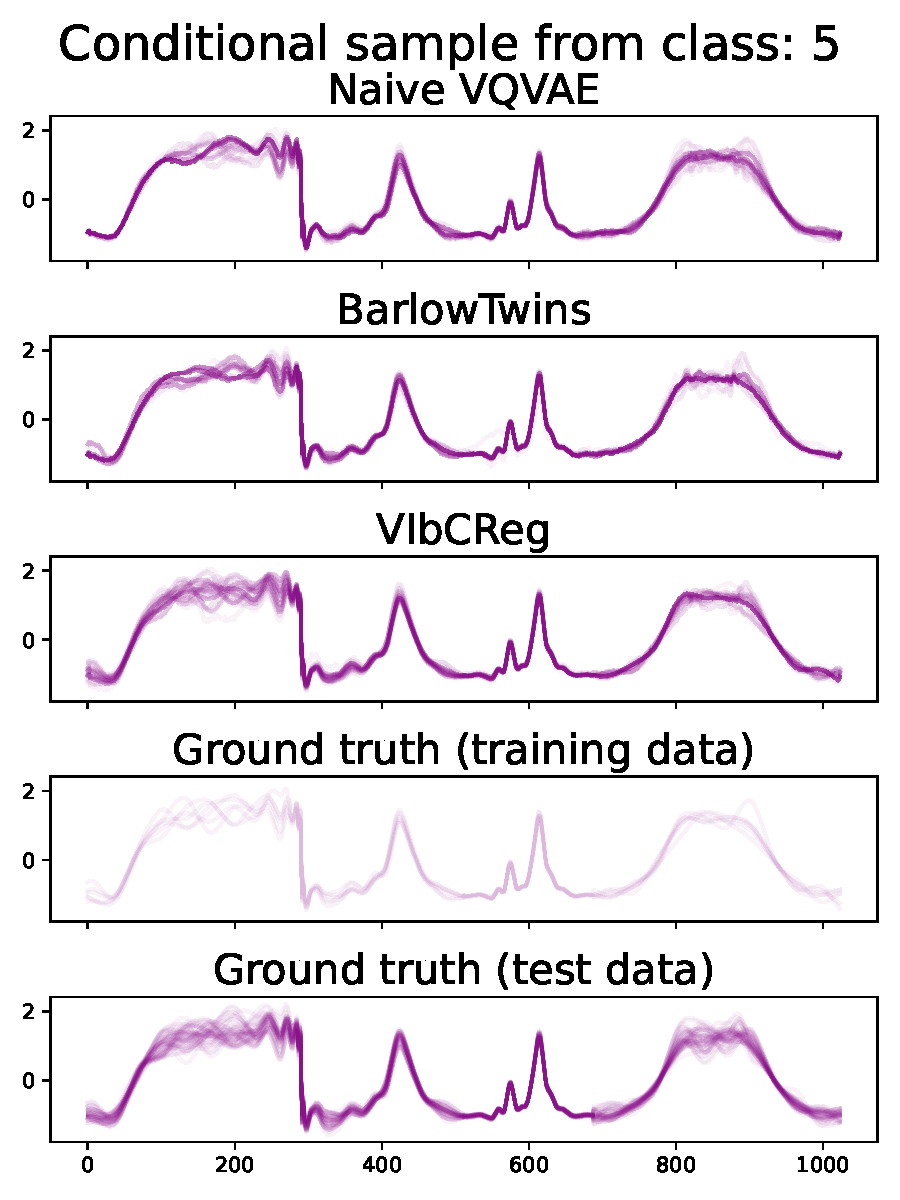
\includegraphics[width=\textwidth]{Mallat-conditional-class5.pdf}
    \end{minipage}
    % \hfill
    \begin{minipage}[b]{0.32\textwidth}
        \centering
        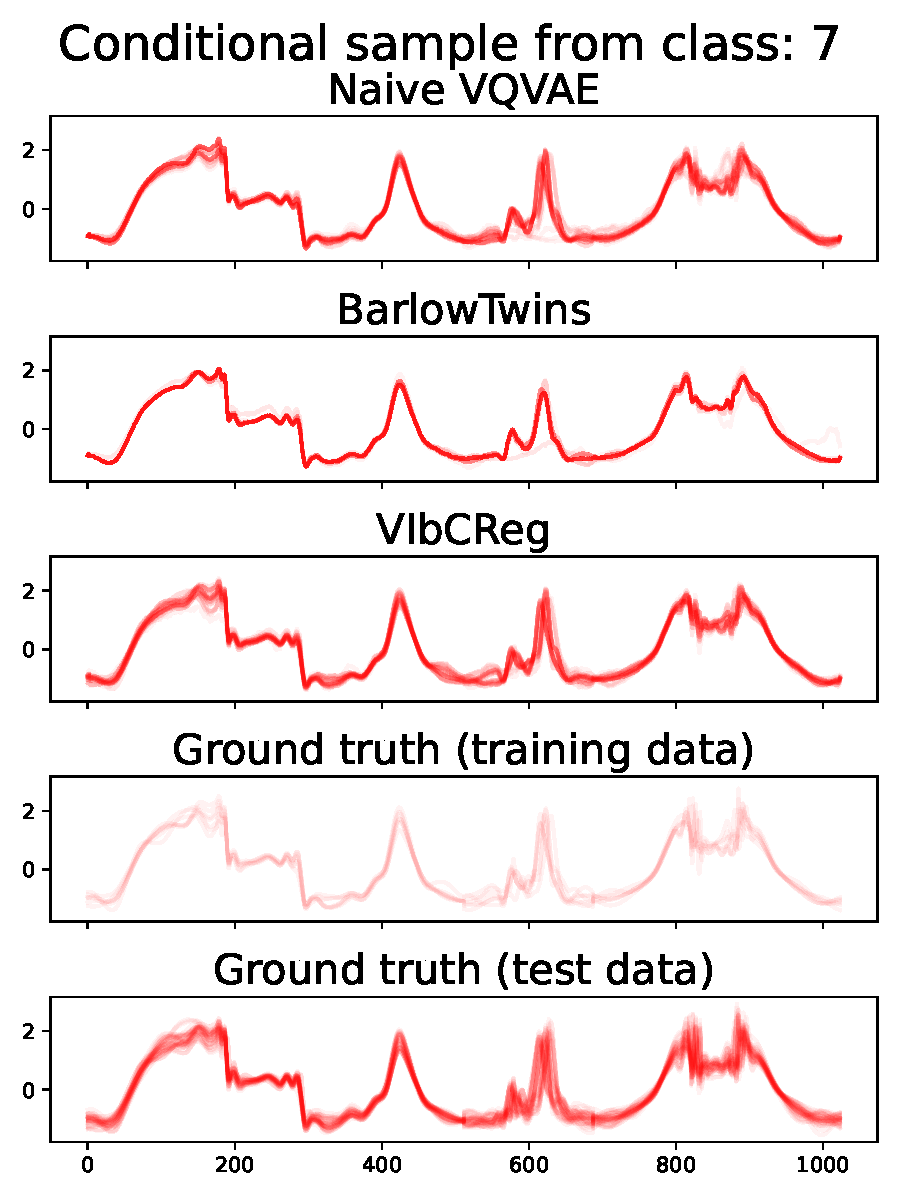
\includegraphics[width=\textwidth]{Mallat-conditional-class7.pdf}
    \end{minipage}
    \begin{minipage}[b]{0.32\textwidth}
        \centering
        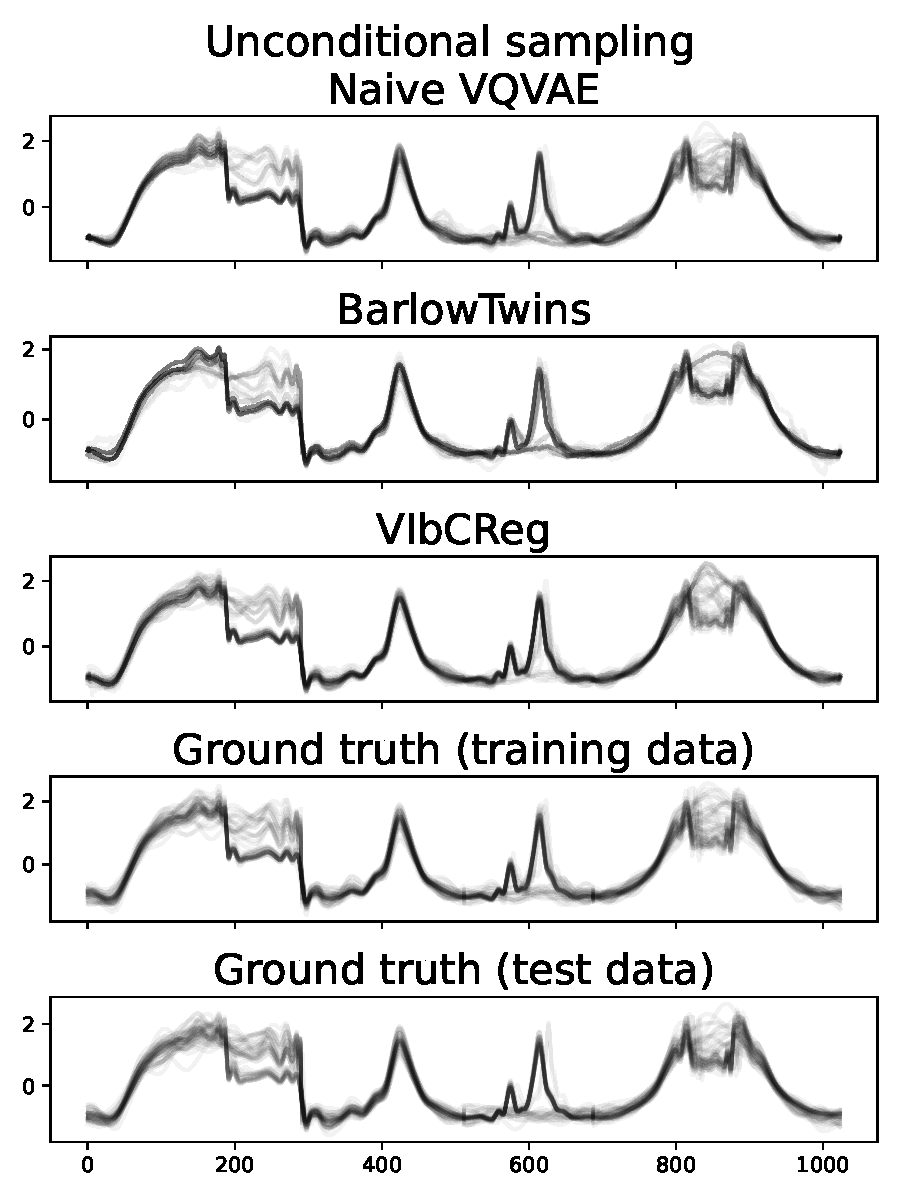
\includegraphics[width=\textwidth]{Mallat-unconditional.pdf}
    \end{minipage}
    \caption{Class conditional distribution for some selected classes of Mallat, in addition to unconditional samples. Barlow and VIbCReg both trained with Gaussian augmentation.}
    \label{fig:Gaussian_Mallat}
\end{figure}

By inspecting the PCA plots of both data space and the discrete latent representations of samples from Mallat, compared to synthetic samples form VIbCReg and Barlow Twins in Figure \ref{fig:Mallat_data_PCA}, we see a clear case of representation collapse for Barlow Twins. We hypothesize that the variance term in VIbCReg assists in maintaining variability in the representations. Making it more effective in avoiding this type of collapse. 

\begin{figure}[h]
    \centering
    % \hfill
    \begin{minipage}[b]{0.40\textwidth}
        \centering
        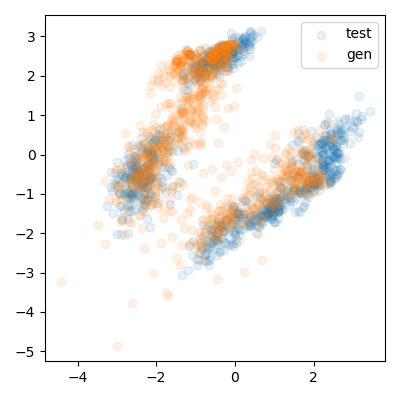
\includegraphics[width=\textwidth]{VIB_gauss_latentspace_PCA_Mallat.png}
    \end{minipage}
    \begin{minipage}[b]{0.40\textwidth}
        \centering
        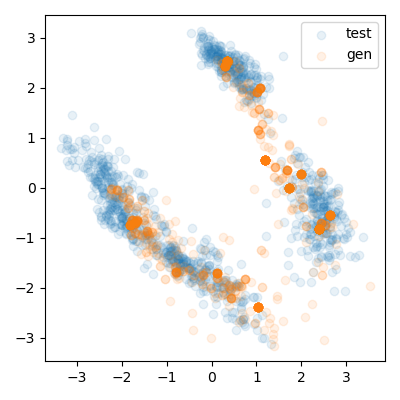
\includegraphics[width=\textwidth]{BT_gauss_latentspace_PCA_Mallat.png}
    \end{minipage}
    \caption{PCA of discrete latent representation from Mallat. Both VIbCReg (left) and Barlow Twins (right) are trained with gaussian augmentation.}
    \label{fig:Mallat_latent_PCA}
\end{figure}

\begin{figure}[h]
    \centering
    % \hfill
    \begin{minipage}[b]{0.40\textwidth}
        \centering
        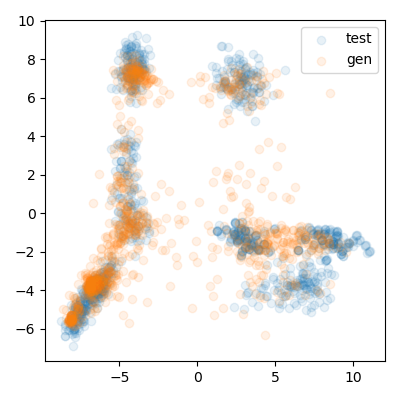
\includegraphics[width=\textwidth]{VIB_gauss_dataspace_PCA_Mallat.png}
    \end{minipage}
    \begin{minipage}[b]{0.40\textwidth}
        \centering
        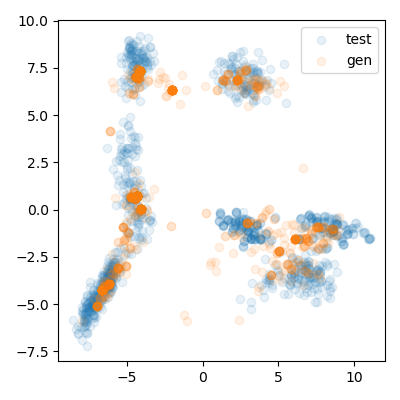
\includegraphics[width=\textwidth]{BT_gauss_dataspace_PCA_Mallat.png}
    \end{minipage}
    \caption{PCA of generated time series from Mallat. Both VIbCReg (left) and Barlow Twins (right) are trained with gaussian augmentation.}
    \label{fig:Mallat_data_PCA}
\end{figure}




\subsubsection{Symbols}

The Symbols dataset consists of several distinct, but simple, patterns. The dataset is very small, where each class contsists of less than 5 training samples.\newline

In Figure \ref{fig:Gauss_Symbols}, particularly the unconditional sample, we see that naive VQVAE does not capture the entire underlying distribution, some classes are not represented/not recognizable, while global consistency for the sinusoids are poor, particularly towards the end. In class 3, we observe that both Barlow Twins and VIbCReg mimic the training data to a large degree. At first glance the naive VQVAE looks to produce the most desirable distribution, but upon closer inspection we see an excessive amount of noise and lack of consistency.\newline

The IS on Symbols, for both VIbCReg and BarlowTwins, is substantially higher than naive VQVAE. While this is not surprising after inspecting the samples, it exposes an issue with the IS metric. It fails to take intraclass diversity into account, and is therefore oblivious to overfitting. \newline

\begin{figure}[H]
    \centering
    \begin{minipage}[b]{0.32\textwidth}
        \centering
        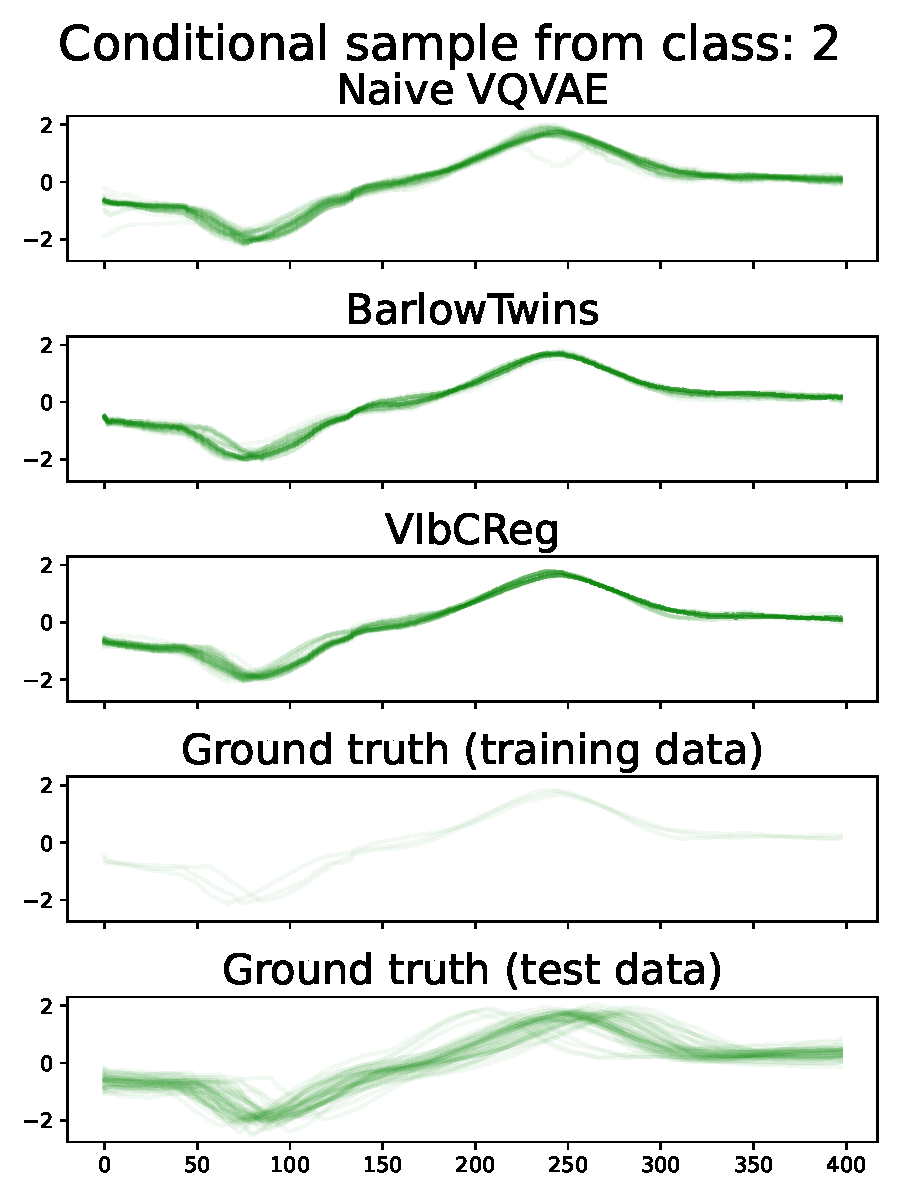
\includegraphics[width=\textwidth]{Symbols-conditional-class2.pdf}
    \end{minipage}
    % \hfill
    \begin{minipage}[b]{0.32\textwidth}
        \centering
        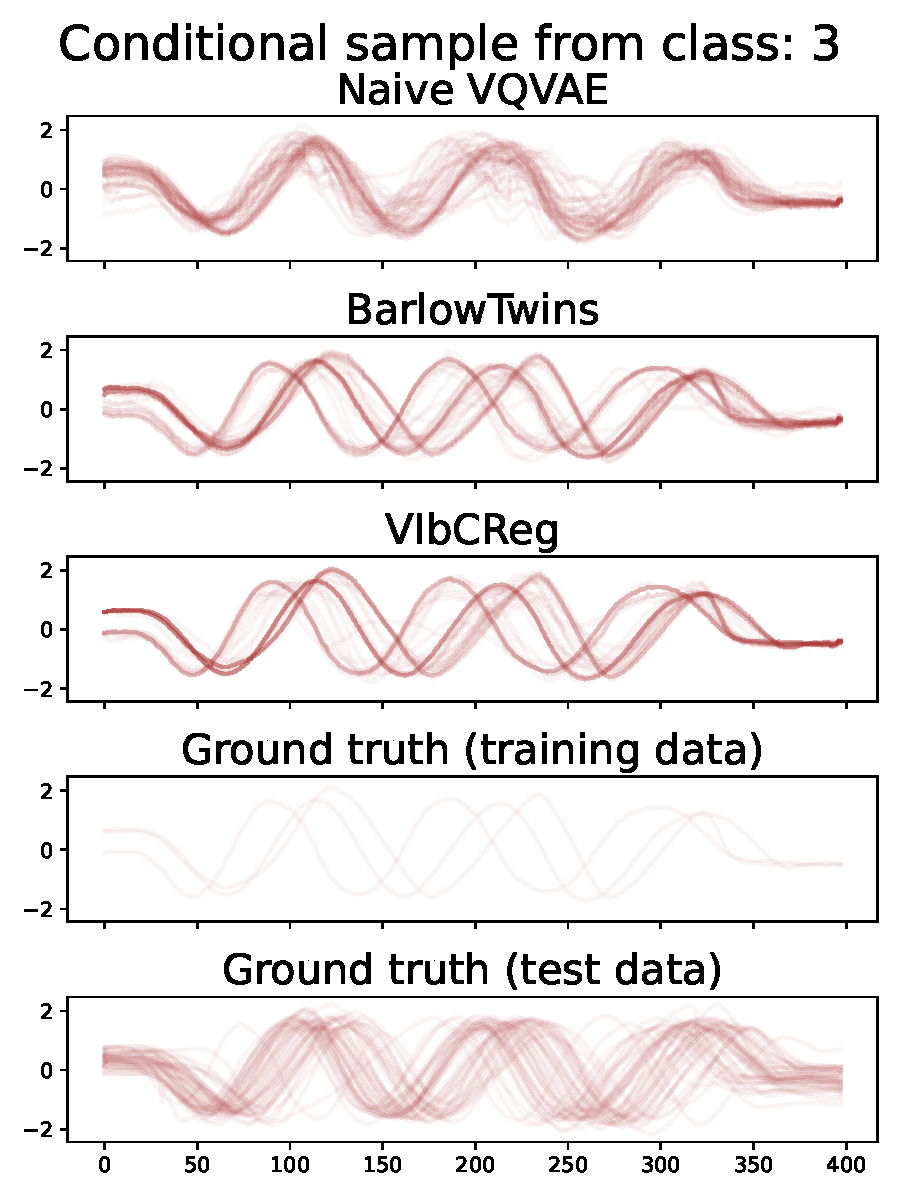
\includegraphics[width=\textwidth]{Symbols-conditional-class3.pdf}
    \end{minipage}
    \begin{minipage}[b]{0.32\textwidth}
        \centering
        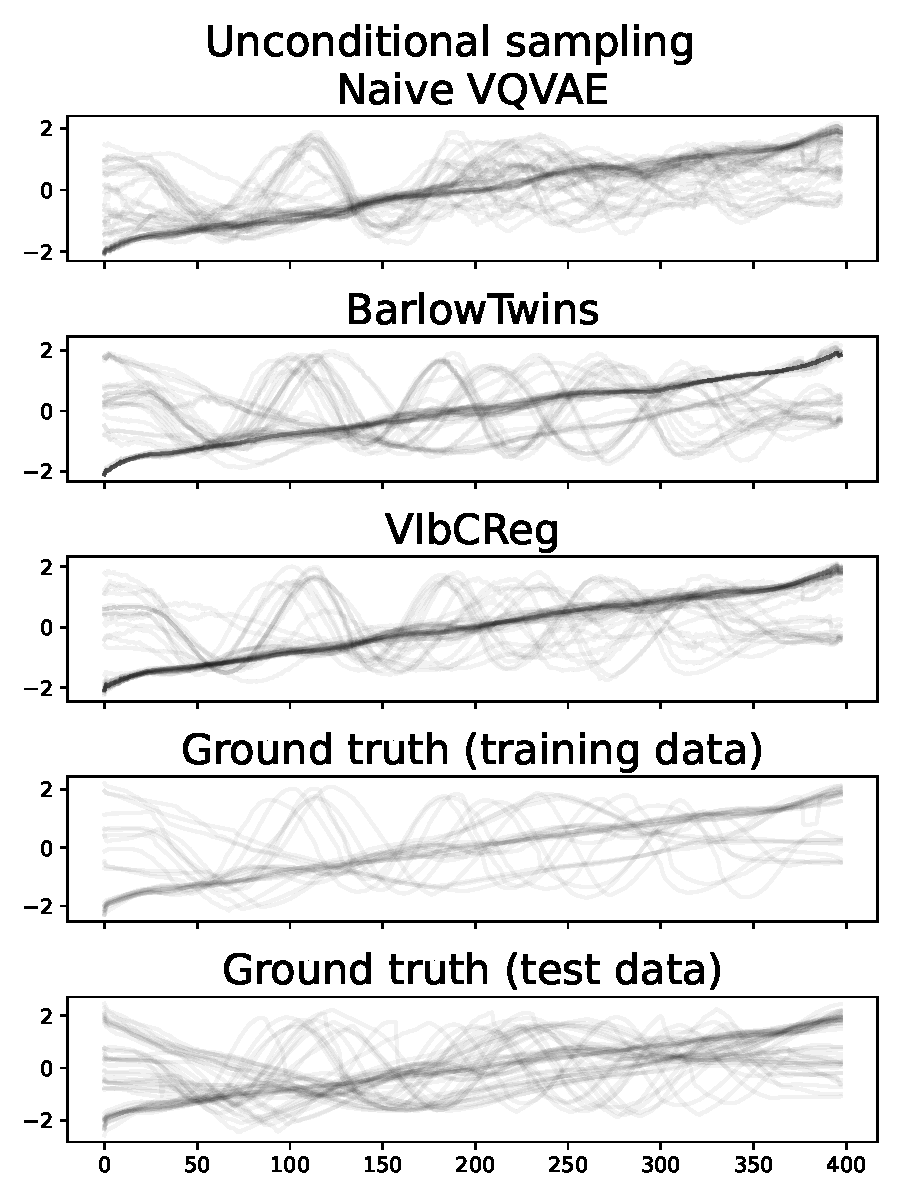
\includegraphics[width=\textwidth]{Symbols-unconditional.pdf}
    \end{minipage}
    \caption{Class conditional distribution for some selected classes of Symbols. Barlow and VIbCReg both trained with gaussian augmentation.}
    \label{fig:Gauss_Symbols}
\end{figure}






\subsubsection{ShapesALL}
The dataset ShapesAll consists of 60 classes, with 10 samples within each class. Each class has distinct patterns, with varying complexity.\newline

In Figure \ref{fig:Gauss_ShapesAll}, we observe clearly that naive VQVAE struggles with capturing the global consistency of the samples. We too observe that Barlow Twins mimic the training slightly more closely than VIbCReg, which provides some insight as to why Barlow Twins improves CAS by about 10 percent compared to naive VQVAE. Both Barlow Twins and VIbCReg improve IS, but fail to improve FID. By inspecting the samples, it is not evident why NC-VQVAE fails to improve FID. As FID is calculated from unconditional samples, the issue is most likely due to a issue not observable from the conditional samples. Most likely an insufficient number of synthetic samples were genereated to represent the large variabilty in the unconditional distribution.   \newline

In Symbols and ECG5000 we saw that NC-VQVAE can overfit when there are very few samples in a class. Reassuringly, the mode coverage is quite good, and similar tendencies are observed for ShapesAll as well. 
\begin{figure}[h]
    \centering
    \begin{minipage}[b]{0.32\textwidth}
        \centering
        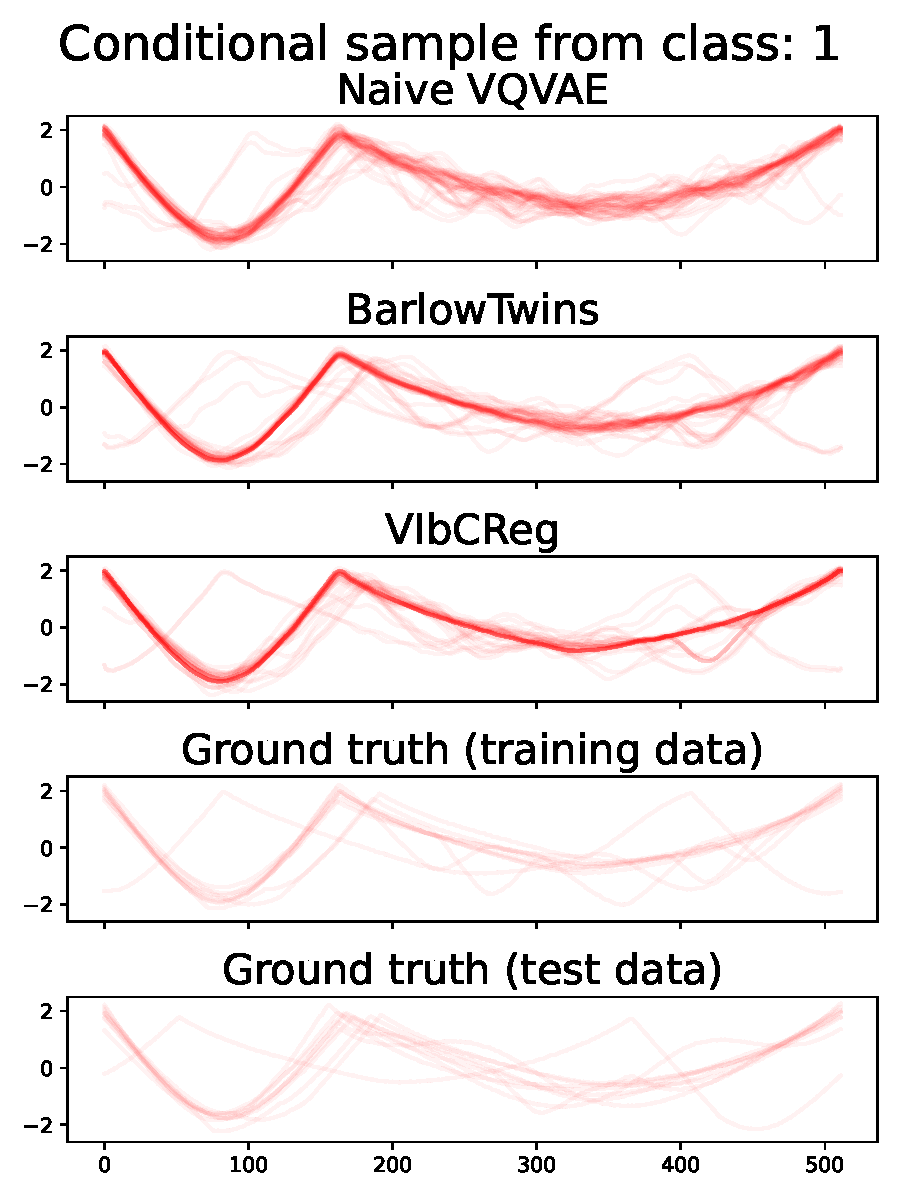
\includegraphics[width=\textwidth]{ShapesAll-conditional-class1.pdf}
    \end{minipage}
    % \hfill
    \begin{minipage}[b]{0.32\textwidth}
        \centering
        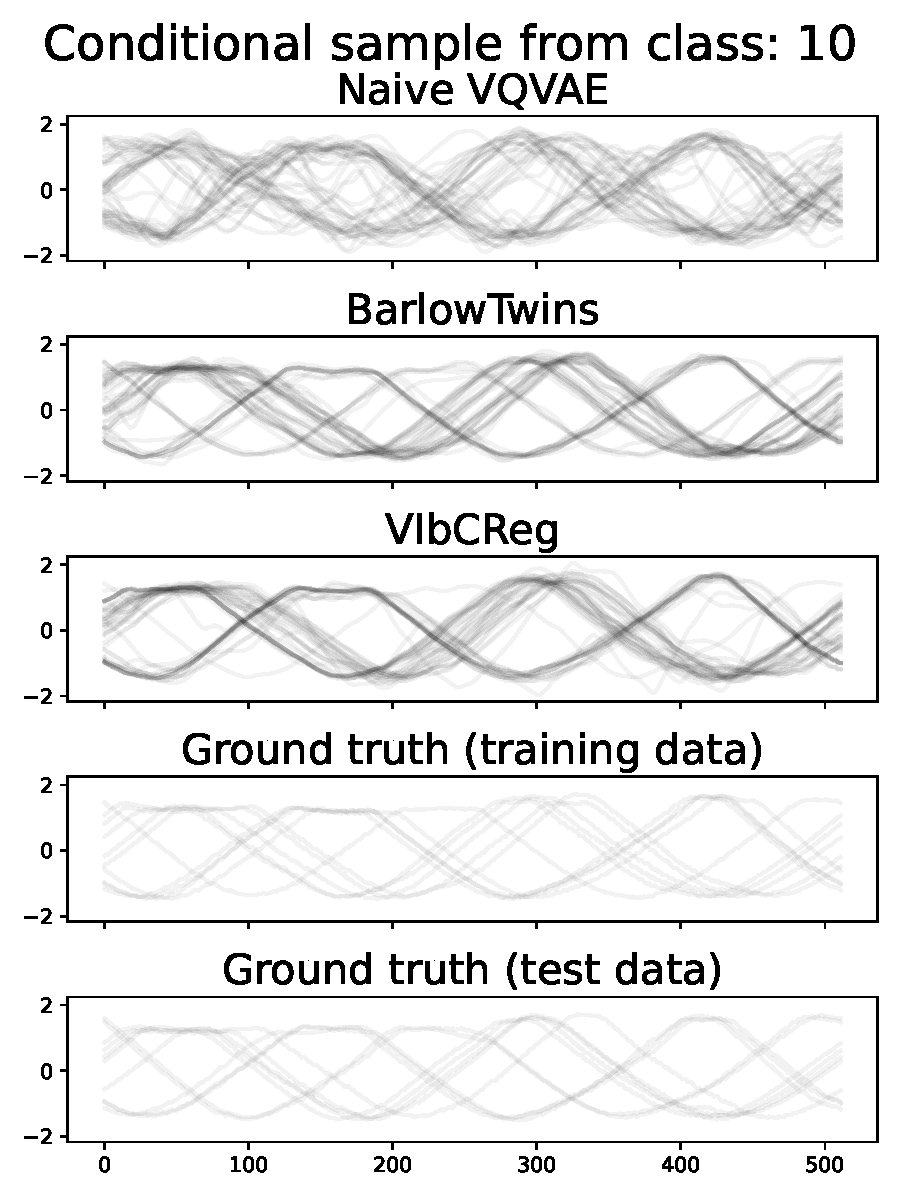
\includegraphics[width=\textwidth]{ShapesAll-conditional-class10.pdf}
    \end{minipage}
    \begin{minipage}[b]{0.32\textwidth}
        \centering
        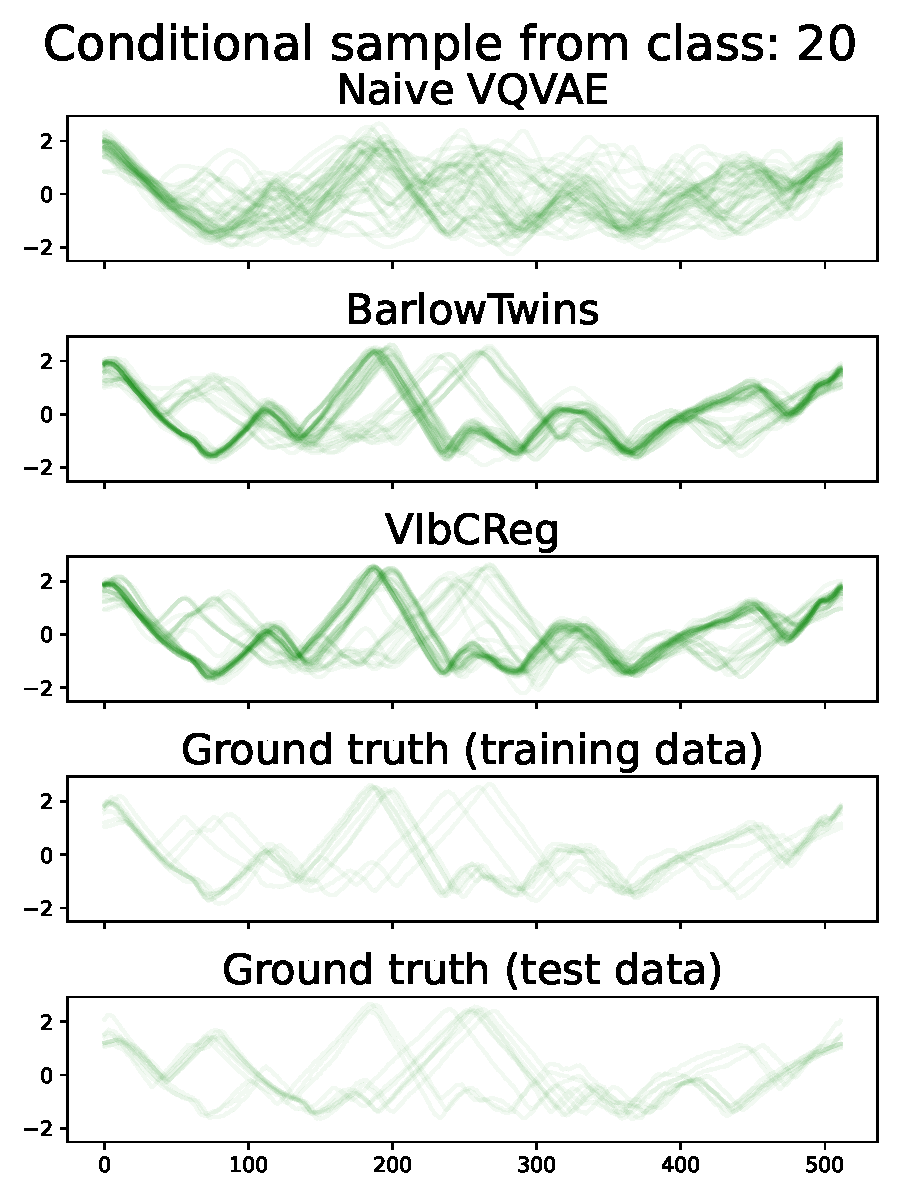
\includegraphics[width=\textwidth]{ShapesAll-conditional-class20.pdf}
    \end{minipage}
    \caption{Class conditional distribution for some selected classes of ShapesAll. Barlow and VIbCReg both trained with gaussian augmentation.}
    \label{fig:Gauss_ShapesAll}
\end{figure}

\subsubsection{UWaveGestureLibraryAll}
The dataset UWaveGestureLibraryAll contains time series with distinct discontinuities and sharp changes in modularity. As noted in \cite{TimeVQVAE}, such datasets are challenging to model.\newline

In Figure \ref{fig:Warp_Uwave} a selected subset of classes are illustrated. We observe upon close inspection that VIbCReg maintains variability in the samples to a greater degree than Barlow Twins, as well at slightly better capturing the dead-spots following the discontinuities.


\begin{figure}[h]
    \centering
    % \hfill
    \begin{minipage}[b]{0.32\textwidth}
        \centering
        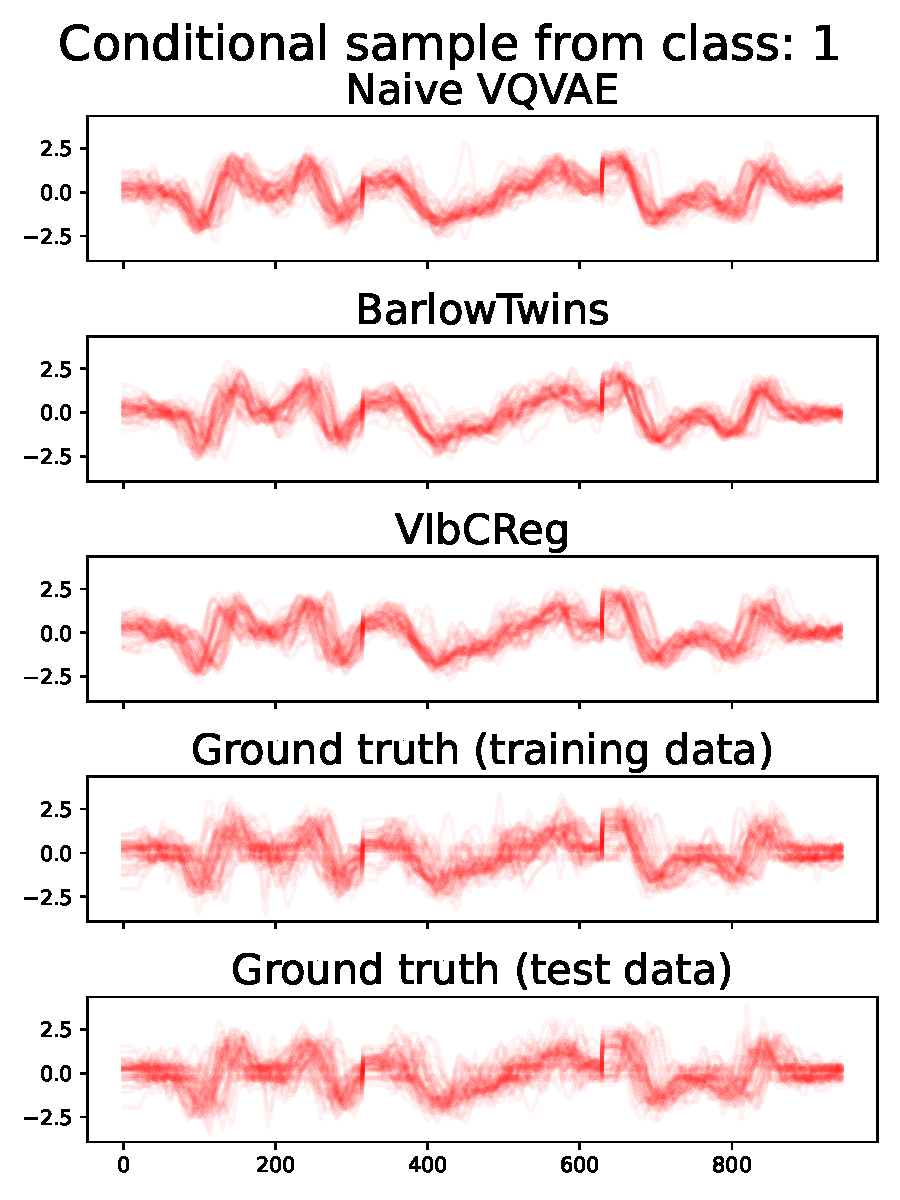
\includegraphics[width=\textwidth]{UWaveGestureLibraryAll-conditional-class1.pdf}
    \end{minipage}
    \begin{minipage}[b]{0.32\textwidth}
        \centering
        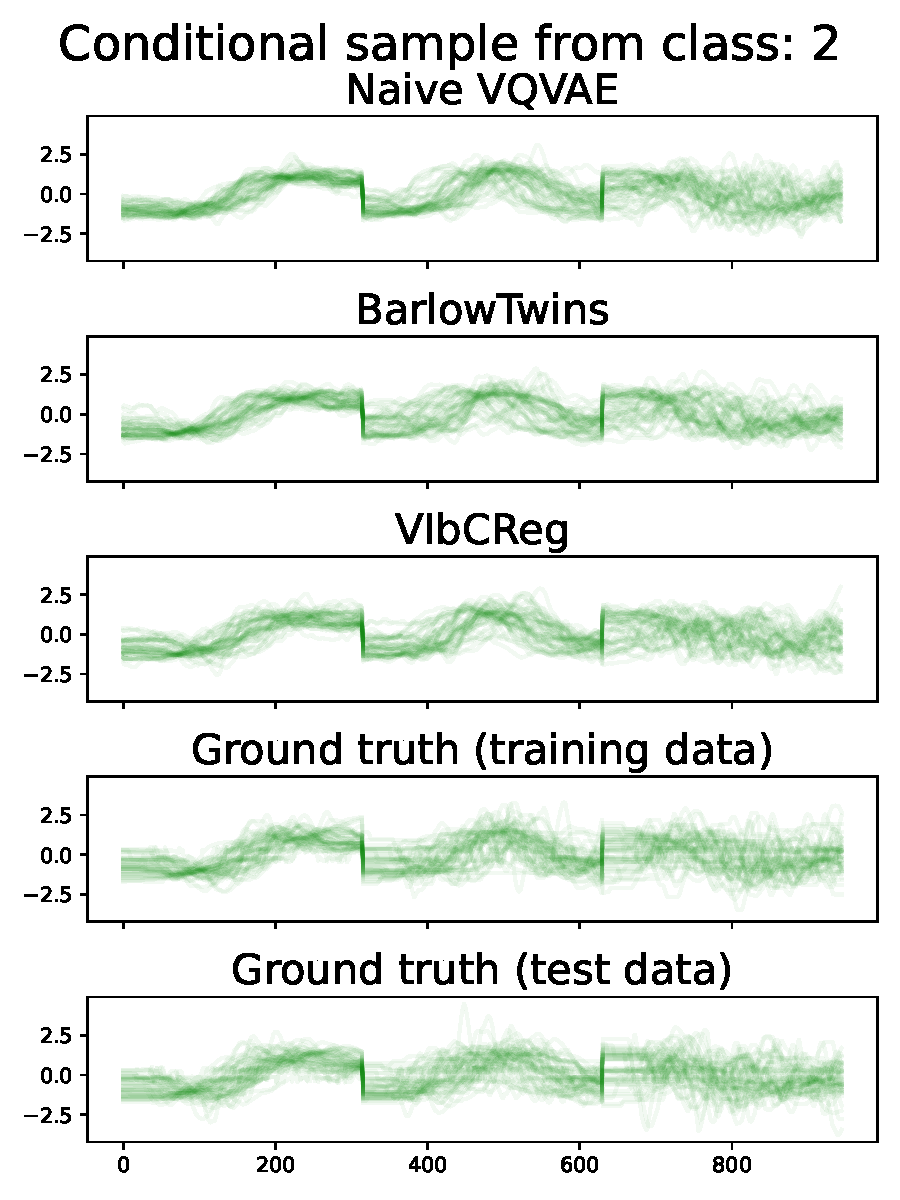
\includegraphics[width=\textwidth]{UWaveGestureLibraryAll-conditional-class2.pdf}
    \end{minipage}
    \begin{minipage}[b]{0.32\textwidth}
        \centering
        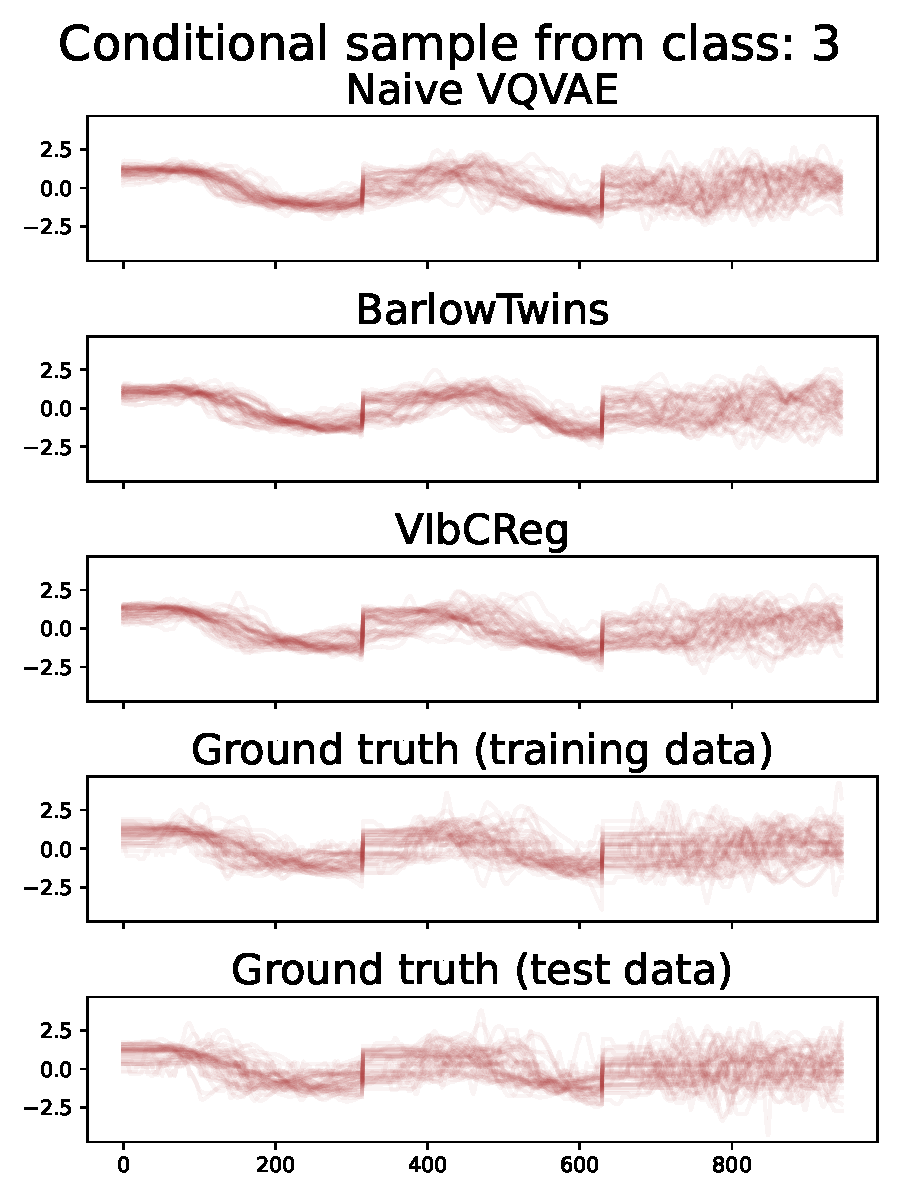
\includegraphics[width=\textwidth]{UWaveGestureLibraryAll-conditional-class3.pdf}
    \end{minipage}
    \caption{Class conditional distribution for some selected classes of UWaveGestureLibraryAll. Barlow and VIbCReg both trained with window warp and amplitude resize augmentations.}
    \label{fig:Warp_Uwave}
\end{figure}



\subsection*{Summary of Stage 2}

In summary, the results from stage 2 suggest that NC-VQVAE offers advantages over the naive VQVAE in capturing conditional distributions, as indicated by higher IS and CAS scores. Additionally, NC-VQVAE demonstrates improved sample quality compared to ground truth data, with lower FID scores. Visual inspections further reveal that NC-VQVAE achieves better mode coverage and captures global sample consistency to a greater extent than its naive counterpart.\newline

Addressing research question 3, we conclude that the expressive representations learned from NC-VQVAE contribute to learning class-specific details and enhancing the quality of synthetic samples. However, it's worth noting that NC-VQVAE is prone to overfitting when faced with small datasets or classes with few samples, whereas the naive VQVAE struggle to capture global consistencies effectively.\newline

Regarding research question 4, we observe that the generative performance is less sensitive to the choice of augmentations compared to the downstream classification accuracy observed in stage 1. Nonetheless, Gaussian noise yields the least variability in performance compared to the baseline, outperforming the naive VQVAE consistently in terms of IS, FID, and CAS metrics.

\section{Ablation Study}
\label{Section:Ablation}
During the development of our model, we investigated the effect of the augmentation reconstruction weight, $\zeta$, both on validation reconstruction and downstream classification. This experiment was carried out on a small scale, focusing on two sets of augmentations: Window Warp and Amplitude Resize, and Slice and Shuffle. We conducted our experiment on a subset of the UCR Archive consisting of FordA, ShapesAll, TwoPatterns and UWaveGestureLibraryAll. The tokenization model underwent training for 250 epochs, with all other parameters maintained as in the main experiment setup. We explored the effect of $\zeta$ across a range of values, specifically $\zeta \in \{0.05, 0.10, 0.15, 0.20\}$. The influence on reconstruction is visualized in Figure \ref{fig:aug_recons_val_recons}, while the impact on KNN and SVM accuracy is presented in Figure \ref{fig:aug_recons_KNN} and \ref{fig:aug_recons_SVM}, respectively.\newline



\begin{figure}[H]
    \centering
    \begin{minipage}[b]{\textwidth}
        \centering
        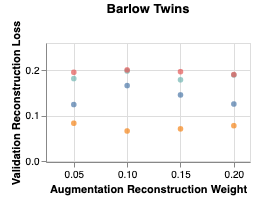
\includegraphics[width=0.35\textwidth]{BT_ValRecons_ReconsWeight.png}
        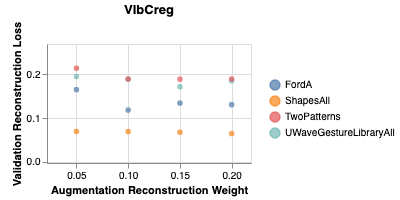
\includegraphics[width=0.55\textwidth]{ViB_ValRecons_ReconsWeight.png}
    \end{minipage}
    \caption*{Augmentation: Window Warp and Amplitude Resize.}
    \begin{minipage}[b]{\textwidth}
        \centering
        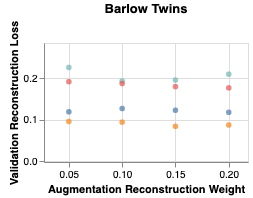
\includegraphics[width=0.35\textwidth]{BT_ValRecons_ReconsWeight_Slice.png}
        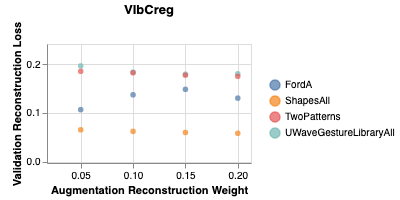
\includegraphics[width=0.55\textwidth]{ViB_ValRecons_ReconsWeight_Slice.png}
    \end{minipage}
    \caption*{Augmentation: Slice and Shuffle.}
    \caption{The effect of the augmentation reconstruction weight on validation reconstruction. Results averaged across 2 runs.}
    \label{fig:aug_recons_val_recons}
\end{figure}


\begin{figure}[H]
    \centering
    % \hfill
    \begin{minipage}[b]{\textwidth}
        \centering
        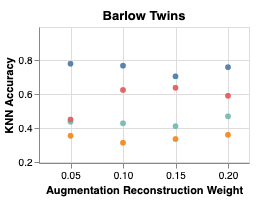
\includegraphics[width=0.35\textwidth]{BT_KNN_ReconsWeight.png}
        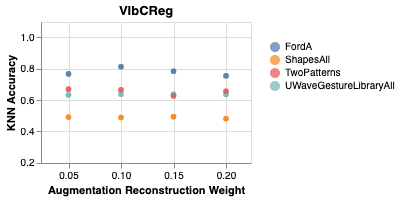
\includegraphics[width=0.55\textwidth]{ViB_KNN_ReconsWeight.png}
    \end{minipage}
    \caption*{Augmentation: Window Warp and Amplitude Resize.}
    \begin{minipage}[b]{\textwidth}
        \centering
        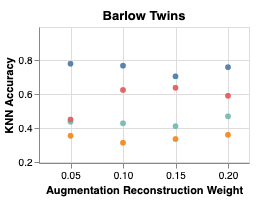
\includegraphics[width=0.35\textwidth]{BT_KNN_ReconsWeight.png}
        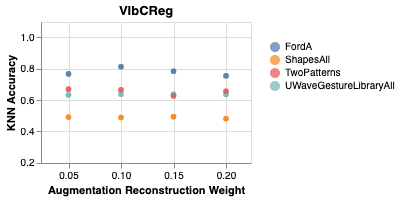
\includegraphics[width=0.55\textwidth]{ViB_KNN_ReconsWeight.png}
    \end{minipage}
    \caption*{Augmentation: Slice and Shuffle.}
    \caption{The effect of the augmentation reconstruction weight on KNN accuracy. Results averaged across 2 runs.}
    \label{fig:aug_recons_KNN}
\end{figure}


\begin{figure}[H]
    \centering
    \begin{minipage}[b]{\textwidth}
        \centering
        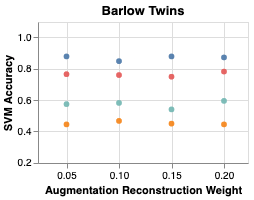
\includegraphics[width=0.35\textwidth]{BT_SVM_ReconsWeight_Slice.png}
        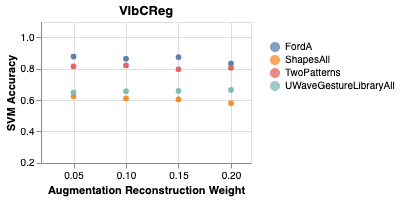
\includegraphics[width=0.55\textwidth]{ViB_SVM_ReconsWeight_Slice.png}
    \end{minipage}
    \caption*{Augmentation: Window Warp and Amplitude Resize.}
    \begin{minipage}[b]{\textwidth}
        \centering
        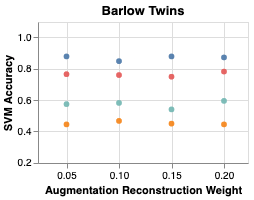
\includegraphics[width=0.35\textwidth]{BT_SVM_ReconsWeight_Slice.png}
        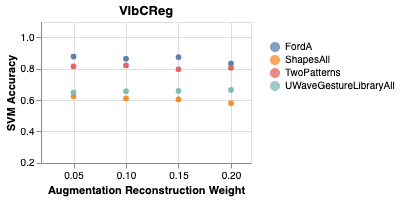
\includegraphics[width=0.55\textwidth]{ViB_SVM_ReconsWeight_Slice.png}
    \end{minipage}
    \caption*{Augmentation: Slice and Shuffle.}
    \caption{The effect of the augmentation reconstruction weight on SVM accuracy. Results averaged across 2 runs.}
    \label{fig:aug_recons_SVM}

\end{figure}

Observing Figure  \ref{fig:aug_recons_val_recons}, we note that the reconstruction loss remains relatively stable across most datasets, exhibiting robustness to variations in the augmentation reconstruction weight. However, FordA displays some degree of variability, and the variability is augmentation dependent. This suggests that when optimizing model performance could benefit from jointly optimizing choice of augmentation and augmentation reconstruction weight. \newline

Examining Figure \ref{fig:aug_recons_KNN} and \ref{fig:aug_recons_SVM}, we observe that augmentation reconstruction weight affects KNN to a larger degree than SVM, indicating that the weight introduces differences in local structure of the discrete latent space, while the global structure is less affected. Furthermore, it's evident that VIbCReg consistently produces high probe accuracies and demonstrates greater robustness compared to Barlow Twins across different augmentation reconstruction weights.

\section{Discussion}
\TODO{Discuss limitations and difficulty in assessing generative models}
The difficulty in visually assessing generative performance for datasets with complicated distributions is still highly relevant.\newline

The lack of large high quality datasets in the time series domain. 

\subsection*{The role of augmentations}
We observe that both probe accuracies and generative scores are dependent on the particular choice of augmentations. The probe accuracies are generally better when augmentation are clearly different from the original view, as for warp and slice, while the generative scores has a tendency to follow the opposite pattern, though not as clearly. Additionally, we have observed that the optimal choice of augmentations is highly dataset dependent, and a systematic analysis of different augmentations on specific datasets is needed to understand the dynamics better.

\subsection*{Temporal vs frequency influence of augmentations}

The Gaussian augmentation introduces a HF component, though its influence in the time domain is visually clear, its affect on the spectrograms is minor, as the LF components typically has much larger magnitude. Window Warp and Amplitude Resize changes LF, often changing the exact location of dominant frequencies on the time axis, but not their order. The effect of Slice and Shuffle is variable, but has a tendency to create sharp discontinuities, which in many cases is a significant HF component.\newline

We assessed and chose our different sets of augmentations based on their effect on the temporal representation on the time series. As we model the time frequency domain, future work should more thoroughly investigate the effects of augmentation on spectrograms. Additionally, all models considered compress the input only along temporal axis in the encoder, which in a sens puts more emphasis in the frequency components rather than the exact temporal structure. 

\subsection*{Differences in Barlow Twins and VIbCReg}

From the visual inspections we observed that VIbCReg maintain the variability in the generated samples a bit better than Barlow Twins. We hypothesize that it is due to the variance term present in VIbCReg, and wonder whether increasing its weight might assist in producing more diverse samples. \newline

In terms of the generative scores, VIbCReg is more robust to choice of augmentations, highlighted by the their different response to the Slice and Shuffle augmentation. This can likely be attributed the difference in variance/covariance regularization on the two models. Since VIbCReg regularizes each branch separately, it responds better to situations where the input of each branch differs significantly. \newline

VIbCReg generally demonstrated slightly better performance in terms of validation reconstruction than Barlow Twins. In the ablation study we observed that VIbCReg was more robust to augmentation reconstruction weight, both in terms of the validation reconstruction and downstream classification.

\subsection*{Overfitting problem}

We have observed on multiple occasions that when the sample size is small and the patterns in the data are simple NC-VQVAE has a tendency to overfit, and memorize the training data to a large degree. In our experiments we have not employed any form of dropout or other regularization techniques when training on small datasets, therefore this issue is to be expected. As the naive VQVAE in the same cases fails to capture the global consistency, we see our model as a step in the right direction, but stress the need for regularization. Additionally, investigating prior learning models and sampling procedures tailored for the more expressive representations, leveraging the encoded semantic information, could be beneficial. 

\subsection*{Training Time and Model Size}
The addition of the self-supervised loss in NC-VQVAE comes at a cost in terms of model size, and consequently training time. The added complexity is a result of the high dimensionality of the projector used in both Barlow Twins and VIbCReg. As the projector is discarded after stage 1, the increased complexity only affect training of the tokenization model. Examining Figure \ref{fig:comp}, we observe a significant increase in training time and trainable parameters.
\begin{figure}[h]
    \centering
    \begin{subfigure}[b]{0.4\textwidth}
        \includegraphics[width=\textwidth]{training_time.pdf}
        \caption{Training time distributions for Stage 1.}
        \label{fig:l}
    \end{subfigure}
    \hspace{0.05\textwidth} % Adjust the horizontal space between columns
    \begin{subfigure}[b]{0.4\textwidth}
        \includegraphics[width=\textwidth]{numparam.png}
        \caption{Number of parameters in Stage 1 for models trained on Wafer.}
        \label{fig:parm}
    \end{subfigure}
    \caption{Overview of training time and model size for Stage 1.}
    \label{fig:comp}
\end{figure}

\end{document}